%definira klasu dokumenta 
\documentclass[12pt]{report} 

%prostor izmedu naredbi \documentclass i \begin{document} se zove uvod. U njemu se nalaze naredbe koje se odnose na cijeli dokument

%osnovni LaTex ne može riješiti sve probleme, pa se koriste različiti paketi koji olakšavaju izradu željenog dokumenta
\usepackage[croatian]{babel} 
\usepackage{amssymb}
\usepackage{amsmath}
\usepackage{txfonts}
\usepackage{mathdots}
\usepackage{titlesec}
\usepackage{array}
\usepackage{lastpage}
\usepackage{etoolbox}
\usepackage{longtable, tabu}
%\usepackage[table]{xcolor}
\usepackage{color, colortbl}

\usepackage{adjustbox}
\usepackage{geometry}
\usepackage[classicReIm]{kpfonts}
\usepackage{hyperref}
\usepackage{fancyhdr}
\usepackage{verbatim}
\usepackage{graphicx}
\graphicspath{{./slike}}
\usepackage{pdflscape}
\usepackage{float}
\usepackage{setspace}
\restylefloat{table}

\usepackage{listings}

\definecolor{dkgreen}{rgb}{0,0.6,0}
\definecolor{gray}{rgb}{0.5,0.5,0.5}
\definecolor{mauve}{rgb}{0.58,0,0.82}

\lstset{
	language=Java,
	aboveskip=3mm,
	belowskip=3mm,
	showstringspaces=false,
	columns=flexible,
	basicstyle={\small\ttfamily},
	numbers=left,
	numberstyle=\tiny\color{gray},
	keywordstyle=\color{blue},
	commentstyle=\color{dkgreen},
	stringstyle=\color{mauve},
	breaklines=true,
	breakatwhitespace=true,
	tabsize=3,
	frame=single,
	captionpos=b,
	escapeinside={\%*}{*)}
}
\renewcommand{\lstlistingname}{Izvorni kod}



\patchcmd{\chapter}{\thispagestyle{plain}}{\thispagestyle{fancy}}{}{} %redefiniranje stila stranice u paketu fancyhdr

%oblik naslova poglavlja
\titleformat{\chapter}{\normalfont\huge\bfseries}{\thechapter.}{20pt}{\Huge}
\titlespacing{\chapter}{0pt}{0pt}{40pt}


\linespread{1.3} %razmak između redaka

\geometry{a4paper, left=1in, top=1in,}  %oblik stranice

\hypersetup{ colorlinks, citecolor=black, filecolor=black, linkcolor=black,	urlcolor=black }   %izgled poveznice


%prored smanjen između redaka u nabrajanjima i popisima
\newenvironment{packed_enum}{
	\begin{enumerate}
		\setlength{\itemsep}{0pt}
		\setlength{\parskip}{0pt}
		\setlength{\parsep}{0pt}
	}{\end{enumerate}}

\newenvironment{packed_item}{
	\begin{itemize}
		\setlength{\itemsep}{0pt}
		\setlength{\parskip}{0pt}
		\setlength{\parsep}{0pt}
	}{\end{itemize}}


%boja za privatni i udaljeni kljuc u tablicama
\definecolor{LightBlue}{rgb}{0.9,0.9,1}
\definecolor{LightGreen}{rgb}{0.9,1,0.9}


%podesavanje zaglavlja i podnožja

\pagestyle{fancy}
\lhead{Programsko inženjerstvo}
\rhead{FringillaSport}
\lfoot{Fringilla}
\cfoot{stranica \thepage/\pageref{LastPage}}
\rfoot{\today}
\renewcommand{\headrulewidth}{0.2pt}
\renewcommand{\footrulewidth}{0.2pt}

\newcommand{\clickablefootnotelink}[2]{\href{#2}{#1}\footnote{\href{#2}{#2}}}

	
\begin{document} 
	
	
	
	\begin{titlepage}
		\begin{center}
			\vspace*{\stretch{1.0}} %u kombinaciji s ostalim \vspace naredbama definira razmak između redaka teksta
			\LARGE Programsko inženjerstvo\\
			\large Ak. god. 2020./2021.\\
			
			\vspace*{\stretch{3.0}}
			
			\huge FringillaSport\\
			\Large Dokumentacija, Rev. \textit{2}\\
			
			\vspace*{\stretch{12.0}}
			\normalsize
			Grupa: \textit{Fringilla}\\
			Voditelj: \textit{Lovro Nuić}\\
			
			
			\vspace*{\stretch{1.0}}
			Datum predaje: \textit{14. 01. 2021.}\\
	
			\vspace*{\stretch{4.0}}
			
			Nastavnik: \textit{Nikolina Frid}\\
		
		\end{center}

	
	\end{titlepage}

	
	\tableofcontents

	\chapter{Dnevnik promjena dokumentacije}
		
		\textbf{\textit{Kontinuirano osvježavanje}}\\
				
		
		\begin{longtabu} to \textwidth {|X[2, l]|X[13, l]|X[3, l]|X[3, l]|}
			\hline \multicolumn{1}{|l|}{\textbf{Rev.}}	& \multicolumn{1}{l|}{\textbf{Opis promjene/dodatka}} & \multicolumn{1}{|l|}{\textbf{Autori}} & \multicolumn{1}{l|}{\textbf{Datum}} \\[3pt] \hline
			\endfirsthead
			
			\hline \multicolumn{1}{|l|}{\textbf{Rev.}}	& \multicolumn{1}{l|}{\textbf{Opis promjene/dodatka}} & \multicolumn{1}{|l|}{\textbf{Autori}} & \multicolumn{1}{l|}{\textbf{Datum}} \\[3pt] \hline
			\endhead
			
			\hline 
			\endlastfoot
			
			0.1 & Napravljen predložak.	& Nuić & 15.10.2020. 		\\[3pt] \hline 
			
			0.2 & Dodani dionici i funkcionalni zahtjevi trenera.	& Marfat & 16.10.2020. 		\\[3pt] \hline 
			
			0.3 & Dodani funkcionalni zahtjevi neprijavljenog korisnika i sportaša i dodan dio obrazaca uporabe.	& Rašić & 16.10.2020. 		\\[3pt] \hline 
			
			0.4 & Uređeni funkcionalni zahtjevi trenera zbog konzistentnosti, dodani funkcionalni zahtjevi baze podataka i dio obrazaca uporabe. & Marfat & 17.10.2020. \\[3pt]
			\hline
			
			0.5 & Dodani funkcionalni zahtjevi i obrasci uporabe za iznajmljivača i administratora. & Ilić & 17.10.2020. \\[3pt]
			\hline
			
			0.6 & Dodani ostali zahtjevi i glavni sudionik u UC20 promijenjen u "Trener". 
			\newline Dodan sekvencijski dijagram za UC6 i postavljen defaultni direktorij za slike u folder "slike". 
			\newline Dodani ostali sekvencijski dijagrami. & Marfat & 31.10.2020. \\[3pt]
			\hline
			
			0.7 & Promijenjeno "Korisnik" u "Sportaš" u obrascima uporabe nakon prijave & Crnogorac & 31.10.2020. \\[3pt]
			\hline
			
			0.8 & U opisu projekta dodana postojeća slična rješenja i moguće nadogradnje projektnog zadatka	& Rašić & 31.10.2020. 		\\[3pt] \hline
			
			0.9 & Dodani UML dijagrami u PNG formatu u direktorij slike te u LaTeX dokument	& Crnogorac & 31.10.2020. 		\\[3pt] \hline
			
			0.10 & Dodan opis projektnog zadatka	& Paradžik & 1.11.2020. 		\\[3pt] \hline
			
			0.11 & Dodan opis baze podataka i relacija	& Srdarev & 2.11.2020. 		\\[3pt] \hline
			
			0.12 & Dodan dijagram baze podataka	& Srdarev & 4.11.2020. 		\\[3pt] \hline
			
			0.13 & Promijenjen UC10	& Marfat & 5.11.2020. 		\\[3pt] \hline
			
			0.14 & Ažuriran dnevnik sastajanja	& Rašić & 8.11.2020 		\\[3pt] \hline 
			
			0.15 & Restrukturirana baza podataka	& Srdarev & 8.11.2020. 		\\[3pt] \hline
			
			0.16 & Ispravak gramatičkih i pravopisnih grešaka	& Paradžik & 8.11.2020 		\\[3pt] \hline 
			
			0.17 & Ažuriran dnevnik sastajanja	& Rašić & 13.11.2020 		\\[3pt] \hline 
			
			0.18 & Uređen stil tablica baze podataka	& Nuić & 13.11.2020 		\\[3pt] \hline 
			
			0.19 & Dijagrami razreda & Nuić & 13.11.2020 		\\[3pt] \hline 
			
			\textbf{1.0} & Verzija samo s bitnim dijelovima za 1. ciklus & Nuić & 13.11.2020. \\[3pt] \hline 
			
			1.1 & Dijagram stanja & Paradžik & 10.01.2021. \\[3pt] \hline
			
			1.2 & Dijagram aktivnosti & Paradžik & 11.01.2021. \\[3pt] \hline
			
			1.3 & Ispravak dokumentacije iz 1. ciklusa & Nuić & 13.01.2021. \\[3pt] \hline 
			
			1.4 & Osvježavanje dijagrama baze podataka & Nuić & 14.01.2021. \\[3pt] \hline

			1.5 & Zaključak i budući rad & Paradžik & 14.01.2021. \\[3pt] \hline
			
			1.6 & Dodan dijagram komponenti i dijagram razmještaja & Crnogorac & 14.01.2020. \\[3pt] \hline
			
			1.7 & Dodani dijagrami razreda & Nuić & 14.01.2021. \\[3pt] \hline
			
			1.8 & Dodane upute za pokretanje & Nuić & 14.01.2021. \\[3pt] \hline
			
			\textbf{2.0} & Završna datoteka za predaju & Nuić & 14.01.2021. \\[3pt] \hline 
		\end{longtabu}
	
	
%		\textit{Moraju postojati glavne revizije dokumenata 1.0 i 2.0 na kraju prvog i drugog ciklusa. Između tih revizija mogu postojati manje revizije već prema tome kako se dokument bude nadopunjavao. Očekuje se da nakon svake značajnije promjene (dodatka, izmjene, uklanjanja dijelova teksta i popratnih grafičkih sadržaja) dokumenta se to zabilježi kao revizija. Npr., revizije unutar prvog ciklusa će imati oznake 0.1, 0.2, …, 0.9, 0.10, 0.11.. sve do konačne revizije prvog ciklusa 1.0. U drugom ciklusu se nastavlja s revizijama 1.1, 1.2, itd.}
	\chapter{Opis projektnog zadatka}

		
		Cilj ovog projekta je timskim radom i korištenjem našeg znanja
		oblikovanja programske potpore razviti web aplikaciju "FringillaSport".
		Cilj aplikacije "FringillaSport" je omogućiti jednostavnije povezivanje sportaša, 
		trenera i iznajmljivača sportskih prostora te taj proces pojednostavniti i ubrzati.
		
		Aplikaciju mogu koristiti i registrirani i neregistrirani korisnici. 
		Registrirani korisnici mogu biti:
		
		\begin{packed_item}
			\item{Administrator}
			\item{Iznajmljivač}
			\item{Trener}
			\item{Sportaš}
		\end{packed_item}
	
		Pri registriranju korisnik bira ulogu Sportaša, Trenera ili Iznajmljivača. Za registraciju Sportaša, Trenera i Iznajmljivača
		su potrebni sljedeći podaci:
		
		\begin{packed_item}
			\item{ime}
			\item{prezime}
			\item{email}
			\item{koriničko ime}
			\item{zaporku}
		\end{packed_item}
	
	Za registraciju Trenera potrebno je još priložiti i službenu dokumentaciju koja potvrđuje da je ta osoba službeni trener za neke sportove 
	(takvu prijavu odobrava administrator koji provjerava vjerodostojnost informacija). 
	
	Mogućnosti korisnika:
	
	\begin{packed_item}
		\item{Neregistrirani korisnik:
			\begin{packed_item}
				\item{Pristup stranici te pristup tražilici sportskih okupljanja/treninga. 
					(Korisnik ima samo pregled, ne može se prijaviti na sportsko okupljanje/trening.)
				}
			\end{packed_item}
		}
	
		\item{Sportaš:
			\begin{packed_item}
				\item{Pristup tražilici sportskih okupljanja/treninga.}
				\item{Prijava za pojedino sportsko okupljanje/trening unutar tražilice sportskih okupljanja/treninga.
				}
				\item{Vidljivost svih prijavljenih događaja u vlastitom kalendaru sportskih okupljanja/treninga.
				}
				\item{Dobivanje preporuke za odabir sporta u kojem bi imao najveće mogućnosti ostvariti izvrsne
					rezultate na natjecanjima. Preporuka se temelji na visini, težini, broju godina i
					ostalih osobnih podataka.}
				\item{Može zatražiti ulogu trenera ako dobije službeni certifikat.
				}
			\end{packed_item}}
	
			\item{Iznajmljivač:
			\begin{packed_item}
				\item{Može imati odvojeni račun trenera/sportaša.}
				\item{Može u uređivaču sportskih objekata dodati svoj sportski objekt navodeći lokaciju, 
					tip sportova koji se mogu u objektu održavati, cijenu po satu, termine dostupne za rezervaciju i 
					dokumentaciju koja potvrđuje da je on vlasnik. (Takvu prijavu administrator provjerava i 
					potvrđuje ako je sve ispravno.)}
				\item{U svom kalendaru može vidjeti trenutno odobrene termine za iznajmljivanje i nove termine za koje
					je netko od korisnika zatražio iznajmljivanje te takve termine odobriti ili odbaciti.
				}
			\end{packed_item}}
		
		\item{Trener:
			\begin{packed_item}
				\item{Može naknadno prijaviti dodatnu službenu dokumentaciju. (Za neki drugi sport ili slično.)
				}
				\item{Mogućnost organiziranja i naplaćivanja treninga u sportovima za koje ima potvrđenu dokumentaciju.
					Trening se može organizirati u uređivaču treninga po istom principu kao što se organizira sportsko
					okupljanje.}
				\item{Nasljeđuje prava sportaša te može organizirati i sportska okupljanja za ostale sportove.
				}
				\item{Uz kalendar sportskih okupljanja na kojima on prisustvuje izvan profesionalnih
					treninga, ima i pristup kalendaru svih svojih termina treninga te podatke o njima.
					 ime}
			\end{packed_item}}
		
		\item{Administrator:
			\begin{packed_item}
				\item{Upravlja sustavom.}
				\item{Odobrava i provjerava istinitost podataka iznajmljivača sportskih objekata i trenera koji se 
					žele registrirati u aplikaciju.}
				\item{Može brisati ili dodavati druge korisnike te im mijenjati uloge. (Brisanjem određenog korisnika, 
					brišu se sve njegove prijave na sportska okupljanja i/ili svi termini treninga kreirani od tog korisnika
					ili/i svi sportski objekti kreirani.)
				}
			\end{packed_item}}
	\end{packed_item}
		
		
		\section{Postojeća slična rješenja}
		
		Aplikacija slična aplikaciji koju mi razvijamo je \clickablefootnotelink{playeasy}{https://www.playeasy.com/}. Playeasy je aplikacija dizajnirana za pretraživanje i iznajmljivanje sportskih objekata ili površina. Pretraživanje je puno detaljnije za razliku od aplikacije koju mi razvijamo s mogućnostima sužavanja rezultata na temelju sporta, tipa prostora (dvorana, auditorij, teretana...), tipa površine (beton, drvo, zemlja...) i drugih.
		
		\begin{figure}[H]
			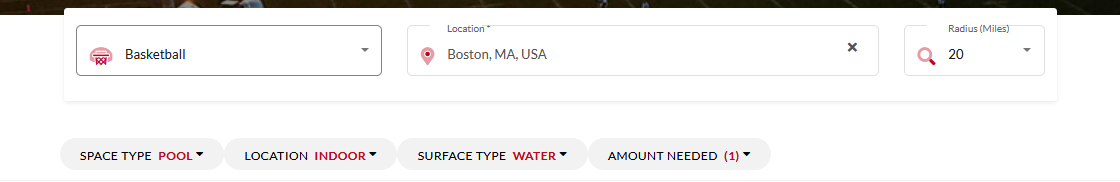
\includegraphics[scale=0.6]{slike/playeasy-pretrazivanje.PNG} %veličina slike u odnosu na originalnu datoteku i pozicija slike
			\centering
			\caption{playeasy - Pretraživanje}
			\label{fig:promjene}
		\end{figure}
		
		Nakon pretraživanja se otvara popis svih dostupnih objekata i površina, te karta s njihovim lokacijama.
		
		\begin{figure}[H]
			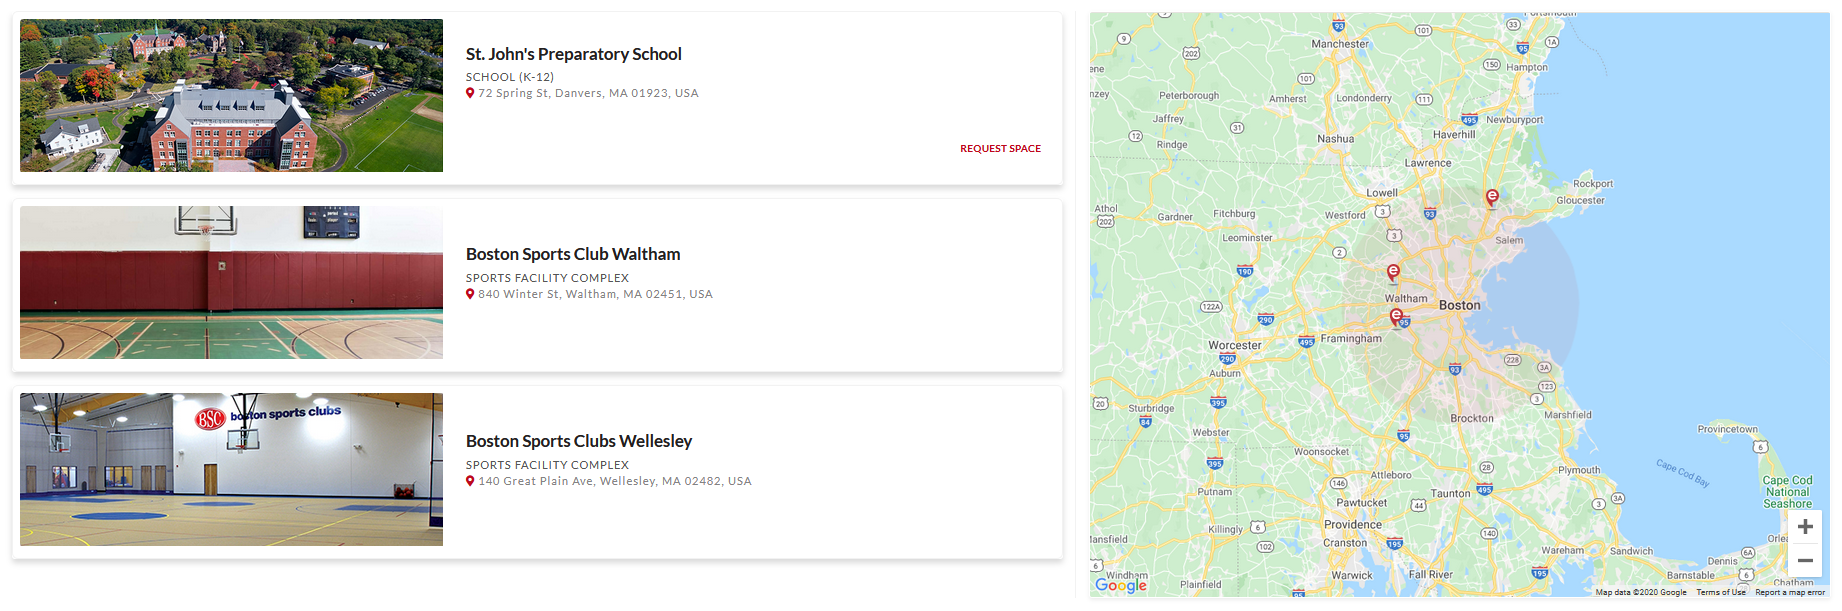
\includegraphics[width=1\linewidth]{slike/playeasy-prikaz.PNG}
			\centering
			\caption{playeasy - Prikaz dostupnih sportskih objekata i površina}
			\label{fig:promjene}
		\end{figure}
		
		Najveća razlika između naše aplikacije i playeasy je što playeasy povezuje samo organizatore sportskih aktivnosti i iznajmljivače, a naša aplikacija povezuje organizatore s iznajmljivačima i sportašima.
		
		Druga slična aplikacija je
		\clickablefootnotelink{teamsnap}{https://www.teamsnap.com/}. Ova aplikacija se fokusira na povezivanje trenera i igrača, te olakšavanje komunikacije između njih. Nema mogućnosti iznajmljivanja sportskih objekata ili površina. Aplikacija sadrži mogućnosti potvrđivanja može li netko doći na trening, grupni chat između članova sportskih ekipa, plaćanje treninga i slične mogućnosti.
		
		\begin{figure}[H]
			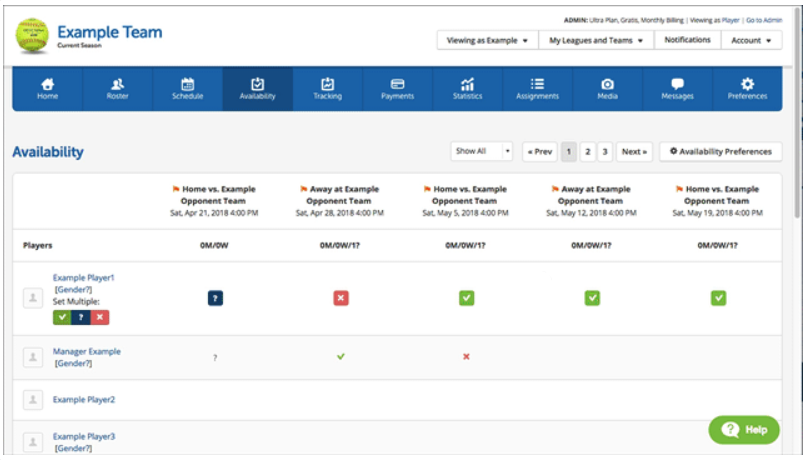
\includegraphics[width=1\linewidth]{slike/teamsnap-dostup.PNG}
			\centering
			\caption{teamsnap - Dostupnost igrača za pojedine sportske događaje}
			\label{fig:promjene}
		\end{figure}
		
		Ostale aplikacije slične našoj su \clickablefootnotelink{uniquevenues}{https://www.uniquevenues.com/} i \clickablefootnotelink{SchoolHire}{https://schoolhire.co.uk/}. Obje ove aplikacije se fokusiraju na iznajmljivanje sportskih površina ili objekata poput aplikacije playeasy, te nemaju mogućnost organiziranja sportskih okupljanja ili treninga.
		
		\section{Moguće nadogradnje projektnog zadatka}
		
		
		Moguća nadogradnja ovog projekta bi bila mogućnost stvaranja sportskih timova. Članovi jednog tima bi mogli međusobno komunicirati, organizirati se i prijavljivati na sportske aktivnosti, te slati upute drugim timovima žele li s njima igrati.
		
		Druga mogućnost bi bila organizacija natjecanja, na koja bi se mogli prijavljivati pojedinci ili timovi ovisno o sportu. Za natjecanje bi se mogao definirati raspored koji bi svi mogli pregledavati, a organizator uređivati.
		
		Još jedna nadogradnja bi mogla biti mogućnost ocjenjivanja trenera, sportskih objekata i površina. Svatko tko je prisustvovao treningu kod nekog trenera ili sportskoj aktivnosti u nekom sportskom objektu ili površini bi mogao ostaviti kratki komentar i ocjenu o tom treneru, sportskom objektu ili površini. 

\iffalse	% zakomentirani primjeri iz latexa, kasnije ukloniti
	
		\section{Primjeri u \LaTeX u}
		
		\textit{Ovo potpoglavlje izbrisati.}\\

		U nastavku se nalaze različiti primjeri kako koristiti osnovne funkcionalnosti \LaTeX a koje su potrebne za izradu dokumentacije. Za dodatnu pomoć obratiti se asistentu na projektu ili potražiti upute na sljedećim web sjedištima:
		\begin{itemize}
			\item Upute za izradu diplomskog rada u \LaTeX u - \url{https://www.fer.unizg.hr/_download/repository/LaTeX-upute.pdf}
			\item \LaTeX\ projekt - \url{https://www.latex-project.org/help/}
			\item StackExchange za Tex - \url{https://tex.stackexchange.com/}\\
		
		\end{itemize} 	


		
		\noindent \underbar{podcrtani tekst}, \textbf{podebljani tekst}, 	\textit{nagnuti tekst}\\
		\noindent \normalsize primjer \large primjer \Large primjer \LARGE {primjer} \huge {primjer} \Huge primjer \normalsize
				
		\begin{packed_item}
			
			\item  primjer
			\item  primjer
			\item  primjer
			\item[] \begin{packed_enum}
				\item primjer
				\item[] \begin{packed_enum}
					\item[1.a] primjer
					\item[b] primjer
				\end{packed_enum}
				\item primjer
			\end{packed_enum}
			
		\end{packed_item}
		
		\noindent primjer url-a: \url{https://www.fer.unizg.hr/predmet/proinz/projekt}
		
		\noindent posebni znakovi: \# \$ \% \& \{ \} \_ 
		$|$ $<$ $>$ 
		\^{} 
		\~{} 
		$\backslash$ 
		
		\begin{longtabu} to \textwidth {|X[8, l]|X[8, l]|X[16, l]|} %definicija širine tablice, širine stupaca i poravnanje
			
			%definicija naslova tablice
			\hline \multicolumn{3}{|c|}{\textbf{naslov unutar tablice}}	 \\[3pt] \hline
			\endfirsthead
			
			%definicija naslova tablice prilikom prijeloma
			\hline \multicolumn{3}{|c|}{\textbf{naslov unutar tablice}}	 \\[3pt] \hline
			\endhead
			
			\hline 
			\endlastfoot
			
			\rowcolor{LightGreen}IDKorisnik & INT	&  	Lorem ipsum dolor sit amet, consectetur adipiscing elit, sed do eiusmod  	\\ \hline
			korisnickoIme	& VARCHAR &   	\\ \hline 
			email & VARCHAR &   \\ \hline 
			ime & VARCHAR	&  		\\ \hline 
			\cellcolor{LightBlue} primjer	& VARCHAR &   	\\ \hline 
			
		\end{longtabu}
		

		\begin{table}[H]
			
			\begin{longtabu} to \textwidth {|X[8, l]|X[8, l]|X[16, l]|} 
				
				\hline 
				\endfirsthead
				
				\hline 
				\endhead
				
				\hline 
				\endlastfoot
				
				\rowcolor{LightGreen}IDKorisnik & INT	&  	Lorem ipsum dolor sit amet, consectetur adipiscing elit, sed do eiusmod  	\\ \hline
				korisnickoIme	& VARCHAR &   	\\ \hline 
				email & VARCHAR &   \\ \hline 
				ime & VARCHAR	&  		\\ \hline 
				\cellcolor{LightBlue} primjer	& VARCHAR &   	\\ \hline 
				
				
			\end{longtabu}
	
			\caption{\label{tab:referencatablica} Naslov ispod tablice.}
		\end{table}
		
		
		%unos slike
		\begin{figure}[H]
			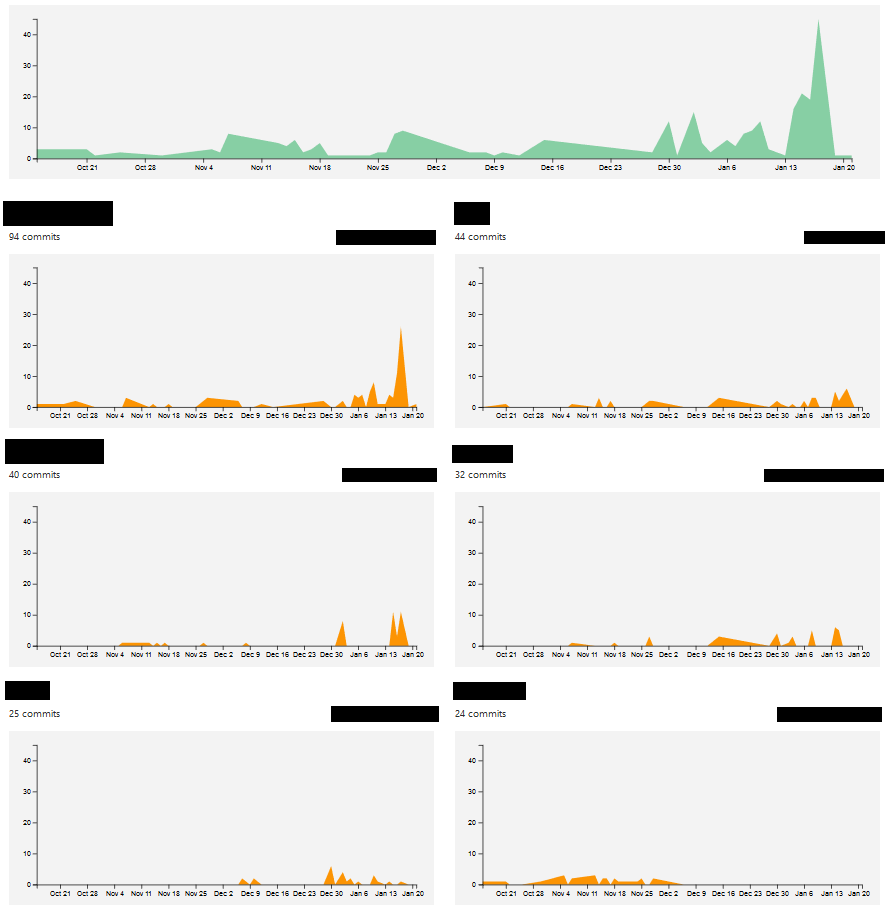
\includegraphics[scale=0.4]{slike/aktivnost.PNG} %veličina slike u odnosu na originalnu datoteku i pozicija slike
			\centering
			\caption{Primjer slike s potpisom}
			\label{fig:promjene}
		\end{figure}
		
		\begin{figure}[H]
			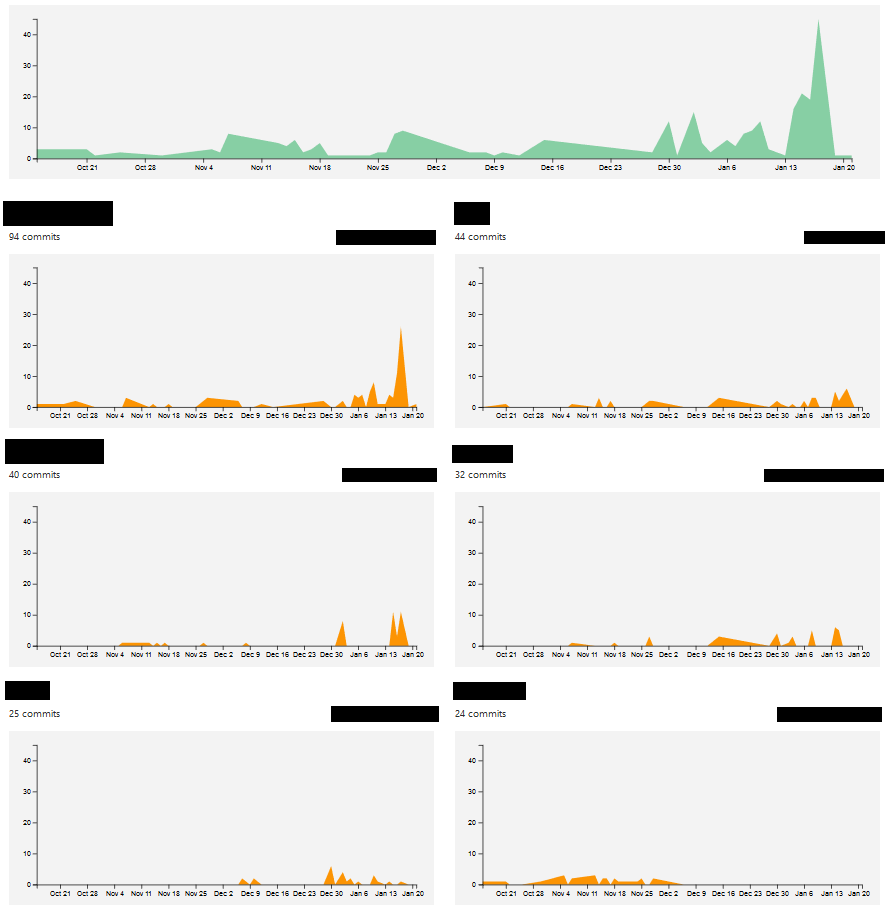
\includegraphics[width=.9\linewidth]{slike/aktivnost.PNG} %veličina u odnosu na širinu linije
			\caption{Primjer slike s potpisom 2}
			\label{fig:promjene2} %label mora biti drugaciji za svaku sliku
		\end{figure}
		
		Referenciranje slike \ref{fig:promjene2} u tekstu.
		
		\eject
\fi	
	\chapter{Specifikacija programske potpore}
		
	\section{Funkcionalni zahtjevi}
			
			\begin{comment}
			\textbf{\textit{dio 1. revizije}}\\
			
			\textit{Navesti \textbf{dionike} koji imaju \textbf{interes u ovom sustavu} ili  \textbf{su nositelji odgovornosti}. To su prije svega korisnici, ali i administratori sustava, naručitelji, razvojni tim.}\\
				
			\textit{Navesti \textbf{aktore} koji izravno \textbf{koriste} ili \textbf{komuniciraju sa sustavom}. Oni mogu imati inicijatorsku ulogu, tj. započinju određene procese u sustavu ili samo sudioničku ulogu, tj. obavljaju određeni posao. Za svakog aktora navesti funkcionalne zahtjeve koji se na njega odnose.}\\
			\end{comment}
			
			\noindent \textbf{Dionici:}
			
			\begin{packed_enum}
				
				\item Sportaš
				\item Trener
				\item Iznajmljivač
				\item Administrator
				\item Razvojni tim
				
			\end{packed_enum}
			
			\noindent \textbf{Aktori i njihovi funkcionalni zahtjevi:}
			
			
			\begin{packed_enum}
				
				\item  \underbar{Neregistrirani/neprijavljeni korisnik (inicijator) može:}
				
				\begin{packed_enum}
					
					\item koristiti tražilicu sportskih okupljanja/treninga
					\item pregledati na karti lokacije sportskih okupljanja/treninga
					\item odabrati sportsko okupljanje/trening i dobiti prikaz informacija o tom sportskom okupljanju/treningu (datum, vrijeme, mjesto, tip sporta)
					\item se registrirati u sustav kao sportaš, trener ili iznajmljivač, za što mu je potrebno ime, prezime, e-mail adresa i lozinka
					
				\end{packed_enum}
				
				
				\item  \underbar{Sportaš (inicijator) može:}
				
				\begin{packed_enum}
					
					\item se prijaviti u aplikaciju
					\item pregledavati i mijenjati osobne podatke
					\item se prijaviti za pojedino sportsko okupljanje/trening
					\item pristupiti kalendaru svih sportskih okupljanja/treninga na koje se prijavio ili koje je organizirao
					\item organizirati sportsko okupljanje za što su mu potrebni datum, vrijeme i mjesto okupljanja, tip sporta te maksimalan broj sudionika
					\item slati upit iznajmljivačima za iznajmljivanje sportskih površina/dvorana
					\item pregledavati sportska okupljanja/treninge predložene od strane aplikacije na temelju sportaševih osobnih podataka
					\item zatražiti da mu se dodijeli uloga trenera
					
				\end{packed_enum}
			
				\item  \underbar{Trener (inicijator) može:}
				
				\begin{packed_enum}
					
					\item se prijaviti u aplikaciju
					\item priložiti službenu dokumentaciju kojom potvrđuje da je trener za određene sportove
					\item pregledavati i mijenjati osobne podatke
					\item se prijaviti za pojedino sportsko okupljanje/trening
					\item slati upit iznajmljivačima za iznajmljivanje sportskih površina/dvorana
					\item organizirati sportska okupljanja za sve sportove i profesionalne (plaćene) treninge za one sportove za koje je potvrđen kao trener za što su mu potrebni datum, vrijeme, mjesto okupljanja, tip sporta te maksimalan broj sudionika
					\item pristupiti kalendaru u kojemu se nalaze sva sportska okupljanja kojima trener prisustvuje i svi njegovi termini treninga i podaci o tim treninzima
					\item koristiti tražilicu sportskih okupljanja/treninga
					
				\end{packed_enum}
			
				\item \underbar{Iznajmljivač (inicijator) može:}
			
				\begin{packed_enum}
				
					\item se prijaviti u aplikaciju
					\item pristupiti uređivaču sportskih objekata u kojemu može mijenjati podatke i termine za već dodane sportske objekte ili dodati novi objekt navodeći lokaciju, tip sportova koji se tamo mogu održavati, cijenu po satu, termine dostupne za rezervaciju i dokumentaciju kojom potvrđuje vlasništvo
					\item pristupiti kalendaru gdje su mu vidljivi svi odobreni termini za iznajmljivanje i novi termini koje su zatražili korisnici koje može odobriti ili odbaciti
					
				\end{packed_enum}
			
				\item \underbar{Administrator (inicijator) može:}
			
				\begin{packed_enum}
				
					\item se prijaviti u aplikaciju
					\item vidjeti sve registrirane korisnike i njihove podatke
					\item odobriti ili odbiti registracije trenera i iznajmljivača na temelju dokumentacije koju prilože
					\item korisnike dodavati, brisati ili im mijenjati razinu pristupa aplikaciji(sportaš, trener, iznajmljivač)
				
				\end{packed_enum}
			
				\item \underbar{Baza podataka (sudionik):}
				
				\begin{packed_enum}
					
					\item pohranjuje sve podatke o korisnicima i njihovim ovlastima
					\item pohranjuje sve podatke o sportskim okupljanjima i profesionalnim treninzima
					\item pohranjuje sve podatke o sportskim objektima koji su prijavljeni u aplikaciji
					
				\end{packed_enum}
			
			\end{packed_enum}
			
			\eject 
			
			
				
			\subsection{Obrasci uporabe}
				
				%\textbf{\textit{dio 1. revizije}}
				
				\subsubsection{Opis obrazaca uporabe}
					\begin{comment}
					\textit{Funkcionalne zahtjeve razraditi u obliku obrazaca uporabe. Svaki obrazac je potrebno razraditi prema donjem predlošku. Ukoliko u nekom koraku može doći do odstupanja, potrebno je to odstupanje opisati i po mogućnosti ponuditi rješenje kojim bi se tijek obrasca vratio na osnovni tijek.}\\
					\end{comment}

					\noindent \underbar{\textbf{UC1 -Pregled sportskih aktivnosti}}
					\begin{packed_item}
						
						\item \textbf{Glavni sudionik: }Korisnik
						\item  \textbf{Cilj:} Pregledati dostupna sportska okupljanja i treninge
						\item  \textbf{Sudionici:} Baza podataka
						\item  \textbf{Preduvjet:} -
						\item  \textbf{Opis osnovnog tijeka:}
						
						\item[] \begin{packed_enum}
							
							\item Karta i tražilica su prikazani prilikom učitavanja aplikacije
							\item Korisnik na karti odabire sportsko okupljanje ili trening
							\item Prikazuju se informacije o odabranom sportskom okupljanju/treningu
						\end{packed_enum}
						
					\end{packed_item}
					
					\noindent \underbar{\textbf{UC2 - Pretraživanje sportskih aktivnosti}}
					\begin{packed_item}
						
						\item \textbf{Glavni sudionik: }Korisnik
						\item  \textbf{Cilj:} Pretraživati dostupna sportska okupljanja i treninge
						\item  \textbf{Sudionici:} Baza podataka
						\item  \textbf{Preduvjet:} -
						\item  \textbf{Opis osnovnog tijeka:}
						
						\item[] \begin{packed_enum}
							
							\item Karta i tražilica su prikazani prilikom učitavanja aplikacije
							\item Korisnik u tražilicu upisuje parametre (mjesto, vrijeme, sport)
							\item Karta se ažurira na temelju unesenih parametara
						\end{packed_enum}
						
					\end{packed_item}
					
					\noindent \underbar{\textbf{UC3 - Registracija}}
					\begin{packed_item}
						
						\item \textbf{Glavni sudionik: }Korisnik
						\item  \textbf{Cilj:} Stvoriti korisnički račun za pristup sustavu
						\item  \textbf{Sudionici:} Baza podataka
						\item  \textbf{Preduvjet:} -
						\item  \textbf{Opis osnovnog tijeka:}
						
						\item[] \begin{packed_enum}
							
							\item Korisnik odabire opciju za registraciju
							\item Korisnik unosi tražene podatke
							\item Korisnik prima obavijest o uspješnoj registraciji
						\end{packed_enum}
						
						\item  \textbf{Opis mogućih odstupanja:}
						
						\item[] \begin{packed_item}
							
							\item[2.a] Odabir već zauzete e-mail adrese, upis podataka u nedozvoljenom formatu, upis neispravne e-mail adrese 
							\item[] \begin{packed_enum}
								
								\item Sustav obavještava korisnika o neuspjeloj registraciji i vraća ga na stranicu za registraciju
								\item Korisnik mijenja neispravno upisane podatke ili odustaje od registracije
								
							\end{packed_enum}
							
						\end{packed_item}
					\end{packed_item}
					
					\noindent \underbar{\textbf{UC4 - Prijava u sustav}}
					\begin{packed_item}
						
						\item \textbf{Glavni sudionik: }Korisnik
						\item  \textbf{Cilj:} Dobiti pristup korisničkom sučelju 
						\item  \textbf{Sudionici:} Baza podataka
						\item  \textbf{Preduvjet:} Registracija
						\item  \textbf{Opis osnovnog tijeka:}
						
						\item[] \begin{packed_enum}
							
							\item Korisnik odabire opciju za prijavu
							\item Korisnik unosi e-mail adresu i lozinku
							\item Potvrda o ispravnosti unesenih podataka
							\item Pristup korisničkim funkcijama
						\end{packed_enum}
						
						\item  \textbf{Opis mogućih odstupanja:}
						
						\item[] \begin{packed_item}
							
							\item[2.a] Neispravna e-mail adresa ili lozinka
							\item[] \begin{packed_enum}
								
								\item Sustav obavještava korisnika o neuspjeloj prijavi i vraća ga na stranicu za prijavu
								\item Korisnik mijenja neispravno unesene podatke ili odustaje od prijave
								
							\end{packed_enum}
							
						\end{packed_item}
					\end{packed_item}
					
					\noindent \underbar{\textbf{UC5 -Pregled osobnih podataka}}
					\begin{packed_item}
						
						\item \textbf{Glavni sudionik: }Sportaš
						\item  \textbf{Cilj:} Pregledati osobne podatke
						\item  \textbf{Sudionici:} Baza podataka
						\item  \textbf{Preduvjet:} Korisnik je prijavljen
						\item  \textbf{Opis osnovnog tijeka:}
						
						\item[] \begin{packed_enum}
							
							\item Korisnik odabire opciju "Osobni podatci"
							\item Prikazuju se osobni podatci korisnika
						\end{packed_enum}
						
					\end{packed_item}
					
					\noindent \underbar{\textbf{UC6 -Promjena osobnih podataka}}
					\begin{packed_item}
						
						\item \textbf{Glavni sudionik: }Sportaš
						\item  \textbf{Cilj:} Promijeniti  osobne podatke
						\item  \textbf{Sudionici:} Baza podataka
						\item  \textbf{Preduvjet:} Korisnik je prijavljen i odabrao je opciju "Osobni podatci"
						\item  \textbf{Opis osnovnog tijeka:}
						
						\item[] \begin{packed_enum}
							
							\item Korisnik odabire opciju za promjenu osobnih podataka
							\item Korisnik mijenja osobne podatke
							\item Korisnik sprema promjene
						\end{packed_enum}
						
					\end{packed_item}
					
					\noindent \underbar{\textbf{UC7 -Prijava na sportsku aktivnost}}
					\begin{packed_item}
						
						\item \textbf{Glavni sudionik: }Sportaš
						\item  \textbf{Cilj:} Prijaviti se na sportsko okupljanje ili trening
						\item  \textbf{Sudionici:} Baza podataka
						\item  \textbf{Preduvjet:} Korisnik je prijavljen
						\item  \textbf{Opis osnovnog tijeka:}
						
						\item[] \begin{packed_enum}
							
							\item Korisnik odabire sportsku aktivnost na koju se želi prijaviti
							\item Korisnik odabire opciju "Prijavi se"
							\item Korisnik potvrdi da se želi prijaviti za odabranu sportsku aktivnost
						\end{packed_enum}
						
					\end{packed_item}
					
					\noindent \underbar{\textbf{UC8 -Pregled prijavljenih sportskih aktivnosti}}
					\begin{packed_item}
						
						\item \textbf{Glavni sudionik: }Sportaš
						\item  \textbf{Cilj:} Pregledati sportska okupljanja ili treninge na koje se korisnik prijavio ili koje je organizirao
						\item  \textbf{Sudionici:} Baza podataka
						\item  \textbf{Preduvjet:} Korisnik je prijavljen
						\item  \textbf{Opis osnovnog tijeka:}
						
						\item[] \begin{packed_enum}
							
							\item Korisnik odabire opciju "Moje prijave"
							\item Prikazuje se kalendar s upisanim terminima svih prijavljenih ili organiziranih sportskih aktivnosti
						\end{packed_enum}
						
					\end{packed_item}
					
					\noindent \underbar{\textbf{UC9 -Organiziranje sportskog okupljanja}}
					\begin{packed_item}
						
						\item \textbf{Glavni sudionik: }Sportaš
						\item  \textbf{Cilj:} Organizirati sportsko okupljanje
						\item  \textbf{Sudionici:} Baza podataka
						\item  \textbf{Preduvjet:} Korisnik je prijavljen
						\item  \textbf{Opis osnovnog tijeka:}
						
						\item[] \begin{packed_enum}
							
							\item Korisnik odabire opciju "Organiziraj sportsko okupljanja"
							\item Korisnik upisuje tražene podatke
							\item Korisnik potvrđuje unesene podatke
							\item Korisnika se preusmjerava na stranicu za pregled prijavljenih sportskih aktivnosti
						\end{packed_enum}
						
						\item  \textbf{Opis mogućih odstupanja:}
						
						\item[] \begin{packed_item}
							
							\item[2.a] Upisano mjesto sportskog okupljanja nije javno i korisnik ga nije iznajmio
							\item[] \begin{packed_enum}
								
								\item Sustav obavještava korisnika da nije iznajmio sportsku površinu/dvoranu te mu daje opciju za iznajmljivanje
								\item Korisnik može promijeniti tražene podatke, odabrati opciju za iznajmljivanje ili odustati od organizacije
								
							\end{packed_enum}
							
						\end{packed_item}
					\end{packed_item}
					
					\noindent \underbar{\textbf{UC10 -Iznajmljivanje sportskih površina/dvorana}}
					\begin{packed_item}
						
						\item \textbf{Glavni sudionik: }Sportaš
						\item  \textbf{Cilj:} Iznajmljivanje sportske površine ili dvorane
						\item  \textbf{Sudionici:} Baza podataka
						\item  \textbf{Preduvjet:} Korisnik je prijavljen i odabrao je opciju "Organiziraj sportsko okupljanje"
						\item  \textbf{Opis osnovnog tijeka:}
						
						\item[] \begin{packed_enum}
							
							\item Korisnik odabire opciju "Iznajmljivanje sportske površine ili dvorane"
							\item Korisnik odabire sportsku površinu ili dvoranu koju želi iznajmiti
							\item Korisnik odabire datum kada želi iznajmiti odabranu sportsku površinu ili dvoranu
							\item Korisniku se prikazuju slobodni termini za odabrani datum
							\item Korisnik odabire željeno vrijeme
							\item Korisnik odabire opciju "Potvrdi rezervaciju"
						\end{packed_enum}
						
						\item  \textbf{Opis mogućih odstupanja:}
						
						\item[] \begin{packed_item}
							
							\item[3.a] Za odabrani datum nema slobodnih termina 
							\item[] \begin{packed_enum}
								
								\item Sustav javlja korisniku da za odabrani datum nema slobodnih termina i daje mu opciju promjene datuma
								
							\end{packed_enum}
							
						\end{packed_item}
						
					\end{packed_item}
					
					\noindent \underbar{\textbf{UC11 -Pregled predloženih aktivnosti }}
					\begin{packed_item}
						
						\item \textbf{Glavni sudionik: }Sportaš
						\item  \textbf{Cilj:} Pregled sportskih aktivnosti predloženih od strane sustava
						\item  \textbf{Sudionici:} Baza podataka
						\item  \textbf{Preduvjet:} Korisnik je prijavljen
						\item  \textbf{Opis osnovnog tijeka:}
						
						\item[] \begin{packed_enum}
							
							\item Korisnik odabire opciju "Predloži za mene"
							\item Sustav prikazuje predložena sportska okupljanja i treninge na temelju osobnih podataka korisnika
							
						\end{packed_enum}
						
					\end{packed_item}
					
					
					
					\noindent \underbar{\textbf{UC12 - Dodavanje sportskog objekta}}
					\begin{packed_item}
						
						\item \textbf{Glavni sudionik: } Iznajmljivač
						\item  \textbf{Cilj:} Dodati novi sportski objekt
						\item  \textbf{Sudionici:} Baza podataka, administrator
						\item  \textbf{Preduvjet:} Korisnik je prijavljen s ovlastima iznajmljivača 
						\item  \textbf{Opis osnovnog tijeka:}
						
						\item[] \begin{packed_enum}
							
							\item Iznajmljivač odabire opciju "Dodaj novi sportski objekt"
							\item Iznajmljivač ispunjava podatke za objekt i prilaže dokumentaciju o vlasništvu
							\item Administrator pregledava i potvrđuje dokumentaciju
							\item Iznajmljivaču se prikazuje poruka o uspješnom dodavanju objekta
							
						\end{packed_enum}
						
						\item  \textbf{Opis mogućih odstupanja:}
						
						\item[] \begin{packed_item}
							
							\item[3.a] Administrator odbija dodavanje objekta zbog nevažeće dokumentacije
							\item[] \begin{packed_enum}
								
								\item Sustav obavještava iznajmljivača o neuspješnom dodavanju objekta
								\item Iznajmljivač može odustati ili ponovno dodati objekt s važećom dokumentacijom
								
							\end{packed_enum}
							
						\end{packed_item}
					
					\end{packed_item}
				
				
				
					\noindent \underbar{\textbf{UC13 - Pregled sportskog objekta}}
					\begin{packed_item}
						
						\item \textbf{Glavni sudionik: } Iznajmljivač
						\item  \textbf{Cilj:}  Pregledati podatke i slobodne termine za sportski objekt
						\item  \textbf{Sudionici:} Baza podataka
						\item  \textbf{Preduvjet:} Korisnik je prijavljen s ovlastima iznajmljivača, administrator mu je odobrio prijavu tog sportskog objekta
						\item  \textbf{Opis osnovnog tijeka:}
						
						\item[] \begin{packed_enum}
							
							\item Iznajmljivač odabire objekt za koji želi pregledati podatke
							\item Prikazuju se podaci i slobodni termini za taj sportski objekt
							
						\end{packed_enum}
						
					\end{packed_item}
					
					
					\noindent \underbar{\textbf{UC14 - Uređivanje sportskog objekta}}
					\begin{packed_item}
						
						\item \textbf{Glavni sudionik: } Iznajmljivač
						\item  \textbf{Cilj:}  Urediti podatke za sportski objekt
						\item  \textbf{Sudionici:} Baza podataka
						\item  \textbf{Preduvjet:} Korisnik je prijavljen s ovlastima iznajmljivača te pregledava podatke i slobodne termine za odabrani sportski objekt.
						\item  \textbf{Opis osnovnog tijeka:}
						
						\item[] \begin{packed_enum}
							
							\item Iznajmljivač odabire "Uredi"
							\item Iznajmljivač mijenja podatke ili slobodne termine za taj objekt
							\item Iznajmljivač odabire opciju "Spremi"
							\item Promjene se spremaju u bazu podataka
							
						\end{packed_enum}
						
						\item  \textbf{Opis mogućih odstupanja:}
						
						\item[] \begin{packed_item}
							
							\item[2.a] Iznajmljivač promjeni podatke, ali ne odabere opciju "Spremi"
							\item[] \begin{packed_enum}
								
								\item Sustav obavještava iznajmljivača da nije spremio podatke prije izlaska iz prozora
							
							\end{packed_enum}
							
						\end{packed_item}
						
					\end{packed_item}
				
					
					\noindent \underbar{\textbf{UC15 - Pregled rezervacija sportskog objekta}}
					\begin{packed_item}
						
						\item \textbf{Glavni sudionik: } Iznajmljivač
						\item  \textbf{Cilj:}  Odobriti nove termine koje su korisnici zatražili i vidjeti već odobrene termine
						\item  \textbf{Sudionici:} Baza podataka
						\item  \textbf{Preduvjet:} Korisnik je prijavljen s ovlastima iznajmljivača 
						\item  \textbf{Opis osnovnog tijeka:}
						
						\item[] \begin{packed_enum}
							
							\item Iznajmljivač odabire kalendar
							\item Iznajmljivač vidi datume s već odobrenim terminima te listu zahtjeva za iznajmljivanjem
							\item Za svaki zahtjev može odabrati "Potvrdi" ili "Odbaci"
							
						\end{packed_enum}
						
					\end{packed_item}
				
				
					\noindent \underbar{\textbf{UC16 - Pregled korisnika}}
					\begin{packed_item}
						
						\item \textbf{Glavni sudionik: } Administrator
						\item  \textbf{Cilj:}  Pregledati registrirane korisnike
						\item  \textbf{Sudionici:} Baza podataka
						\item  \textbf{Preduvjet:} Korisnik je prijavljen s ovlastima administratora 
						\item  \textbf{Opis osnovnog tijeka:}
						
						\item[] \begin{packed_enum}
							
							\item Administrator odabire opciju pregledavanja registriranih korisnika
							\item Sustav prikazuje listu registriranih korisnika
							
						\end{packed_enum}
					
					\end{packed_item}
				
					\noindent \underbar{\textbf{UC17 - Brisanje korisnika}}
					\begin{packed_item}
					
						\item \textbf{Glavni sudionik: } Administrator
						\item  \textbf{Cilj:}  Obrisati registriranog korisnika
						\item  \textbf{Sudionici:} Baza podataka
						\item  \textbf{Preduvjet:} Korisnik je prijavljen s ovlastima administratora i odabrao je opciju pregleda registriranih korisnika
						\item  \textbf{Opis osnovnog tijeka:}
					
						\item[] \begin{packed_enum}
						
							\item Administrator iz liste bira korisnika kojeg želi izbrisati
							\item Odabirom opcije "Obriši" briše se korisnik te sve njegove prijave na sportske aktivnosti, njegovi sportski objekti te svi treninzi koje je organizirao
						
						\end{packed_enum}
					
					\end{packed_item}
				
						\noindent \underbar{\textbf{UC18 - Promjena prava pristupa}}
					\begin{packed_item}
						
						\item \textbf{Glavni sudionik: } Administrator
						\item  \textbf{Cilj:}  Promijeniti prava pristupa registriranom korisniku
						\item  \textbf{Sudionici:} Baza podataka
						\item  \textbf{Preduvjet:} Korisnik je prijavljen s ovlastima administratora i odabrao je opciju pregleda registriranih korisnika
						\item  \textbf{Opis osnovnog tijeka:}
						
						\item[] \begin{packed_enum}
							
							\item Administrator iz liste bira korisnika kojemu želi promijeniti ovlasti
							\item Administrator bira koju razinu ovlasti daje odabranom korisniku
							
						\end{packed_enum}
						
					\end{packed_item}
			
						\noindent \underbar{\textbf{UC19 - Pregled zahtjeva }}
					\begin{packed_item}
						
						\item \textbf{Glavni sudionik: } Administrator
						\item  \textbf{Cilj:}  Odobriti ili odbaciti zahtjeve za registraciju trenera i zahtjeve iznajmljivača za dodavanje sportskog objekta
						\item  \textbf{Sudionici:} Baza podataka
						\item  \textbf{Preduvjet:} Korisnik je prijavljen s ovlastima administratora 
						\item  \textbf{Opis osnovnog tijeka:}
						
						\item[] \begin{packed_enum}
							
							\item Administrator odabire opciju pregledavanja zahtjeva
							\item Administrator uz svaki zahtjev ima opciju dohvaćanja priložene dokumentacije
							\item Administrator nakon pregleda dokumentacije zahtjeva bira "Potvrdi" ili "Odbaci"
							
						\end{packed_enum}
						
					\end{packed_item}
					
					\noindent \underbar{\textbf{UC20 -Organiziranje profesionalnog treninga}}
					\begin{packed_item}
						
						\item \textbf{Glavni sudionik: }Trener
						\item  \textbf{Cilj:} Organizirati profesionalni trening
						\item  \textbf{Sudionici:} Baza podataka
						\item  \textbf{Preduvjet:} Korisnik je prijavljen i odobrena mu je licenca trenera za određeni sport
						\item  \textbf{Opis osnovnog tijeka:}
						
						\item[] \begin{packed_enum}
							
							\item Korisnik odabire opciju "Organiziraj profesionalni trening"
							\item Korisnik upisuje tražene podatke
							\item Korisnik potvrđuje upisane podatke
							\item Korisnika se preusmjerava na stranicu za pregled prijavljenih sportskih aktivnosti
							
						\end{packed_enum}
						
						\item  \textbf{Opis mogućih odstupanja:}
						
						\item[] \begin{packed_item}
							
							\item[2.a] Upisano mjesto profesionalnog treninga nije javno i korisnik ga nije iznajmio
							\item[] \begin{packed_enum}
								
								\item Sustav obavještava korisnika da nije iznajmio sportsku površinu/dvoranu te mu daje opciju za iznajmljivanje
								\item Korisnik može promijeniti tražene podatke, odabrati opciju za iznajmljivanje ili odustati od organizacije
								
							\end{packed_enum}
							
						\end{packed_item}
					\end{packed_item}
					
					\noindent \underbar{\textbf{UC21 -Prilaganje službene dokumentacije}}
					\begin{packed_item}
						
						\item \textbf{Glavni sudionik: }Sportaš
						\item  \textbf{Cilj:} Dobiti odgovarajuću ulogu i odgovarajuće ovlasti
						\item  \textbf{Sudionici:} Baza podataka, Administrator
						\item  \textbf{Preduvjet:} Korisnik je prijavljen
						\item  \textbf{Opis osnovnog tijeka:}
						
						\item[] \begin{packed_enum}
							
							\item Korisnik odabire opciju "Dodaj službenu dokumentaciju"
							\item Korisnik upisuje tražene podatke
							\item Korisnik potvrđuje upisane podatke
							\item Administrator zaprima prijavu
							\item Korisnika se preusmjerava na stranicu kojom se korisniku daje do znanja da je njegova prijava zaprimljena te da će biti obaviješten kada ona bude obrađena
							
						\end{packed_enum}
						
					\end{packed_item}
					
%					\noindent \underbar{\textbf{UC$<$broj obrasca$>$ -$<$ime obrasca$>$}}
%					\begin{packed_item}
%						
%						\item \textbf{Glavni sudionik: }$<$sudionik$>$
%						\item  \textbf{Cilj:} $<$cilj$>$
%						\item  \textbf{Sudionici:} $<$sudionici$>$
%						\item  \textbf{Preduvjet:} $<$preduvjet$>$
%						\item  \textbf{Opis osnovnog tijeka:}
						
%						\item[] \begin{packed_enum}
							
%							\item $<$opis korak jedan$>$
%							\item $<$opis korak dva$>$
%							\item $<$opis korak tri$>$
%							\item $<$opis korak četiri$>$
%						\end{packed_enum}
						
%						\item  \textbf{Opis mogućih odstupanja:}
						
%						\item[] \begin{packed_item}
							
%							\item[2.a] $<$opis mogućeg scenarija odstupanja u koraku 2$>$
%							\item[] \begin{packed_enum}
								
%								\item $<$opis rješenja mogućeg scenarija korak 1$>$
%							\item $<$opis rješenja mogućeg scenarija korak 2$>$
								
							%\end{packed_enum}
							%\item[2.b] $<$opis mogućeg scenarija odstupanja u koraku 2$>$
							%\item[3.a] $<$opis mogućeg scenarija odstupanja  u koraku 3$>$
%							
%						\end{packed_item}
%					\end{packed_item}
				
					
				\subsubsection{Dijagrami obrazaca uporabe}
					
					%\textit{Prikazati odnos aktora i obrazaca uporabe odgovarajućim UML dijagramom. Nije nužno nacrtati sve na jednom dijagramu. Modelirati po razinama apstrakcije i skupovima srodnih funkcionalnosti.}
					\begin{figure}[H]
						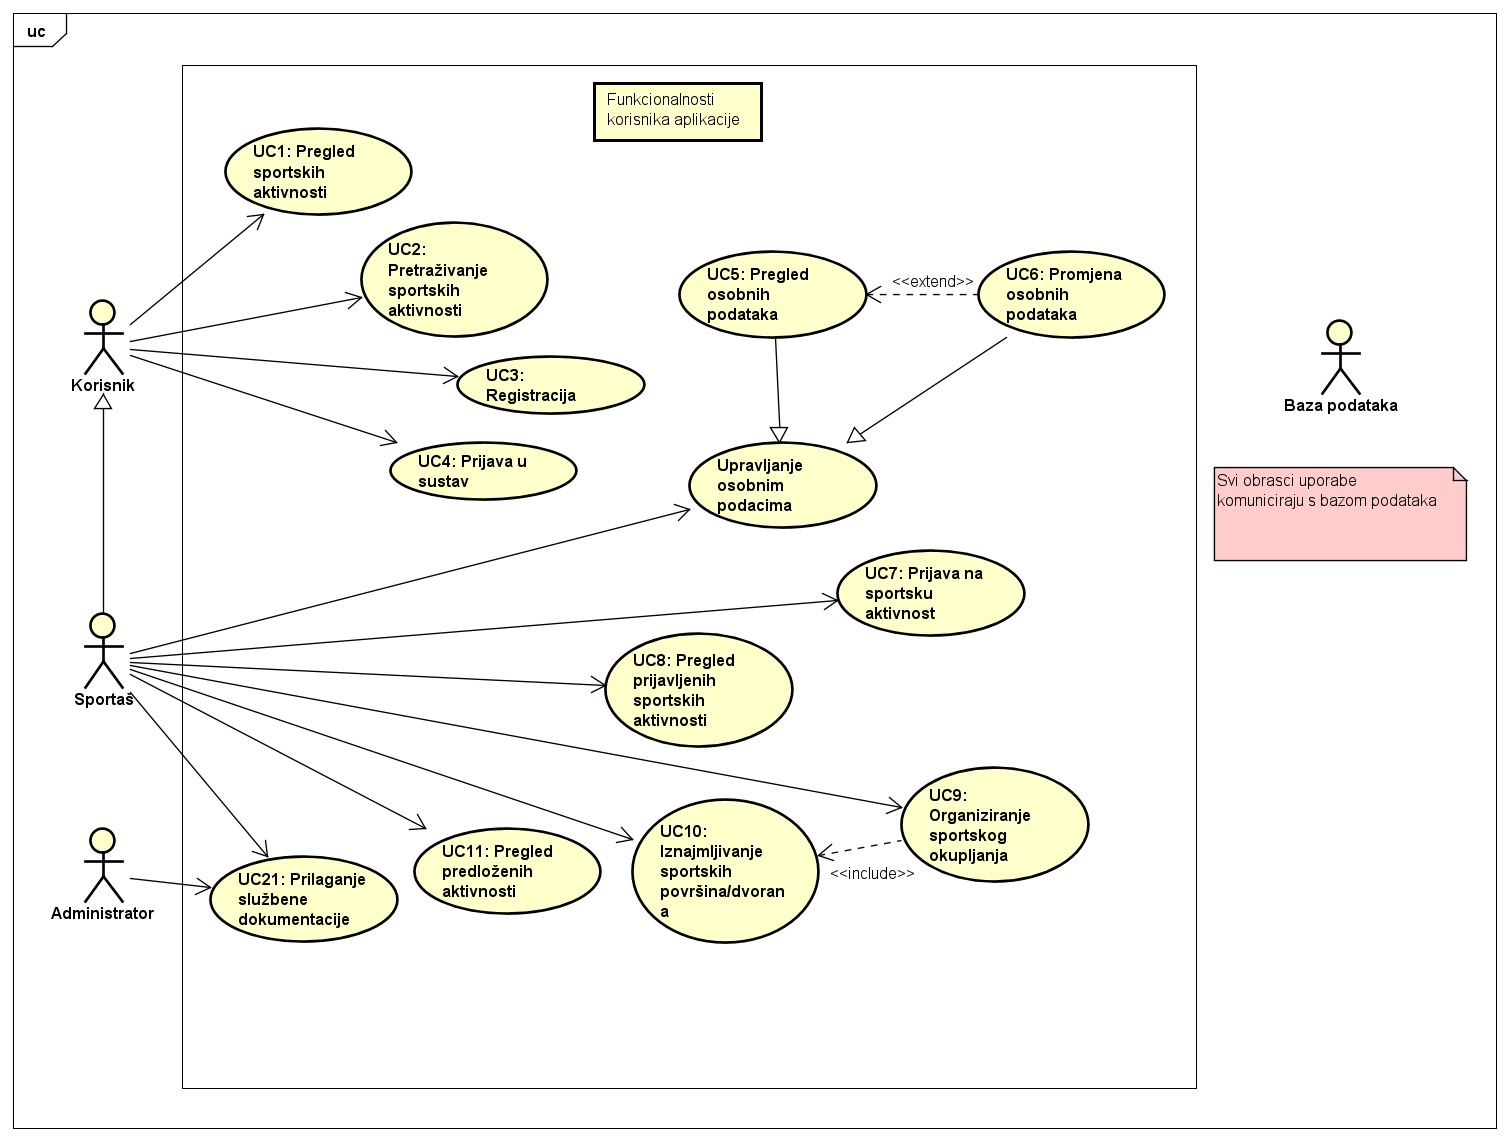
\includegraphics[width=1\linewidth]{slike/KorisnikSportas.PNG}
						\centering
						\caption{Funkcionalnosti korisnika aplikacije}
						\label{fig:funkcionalnosti_korisnik}
					\end{figure}
					\begin{figure}[H]
						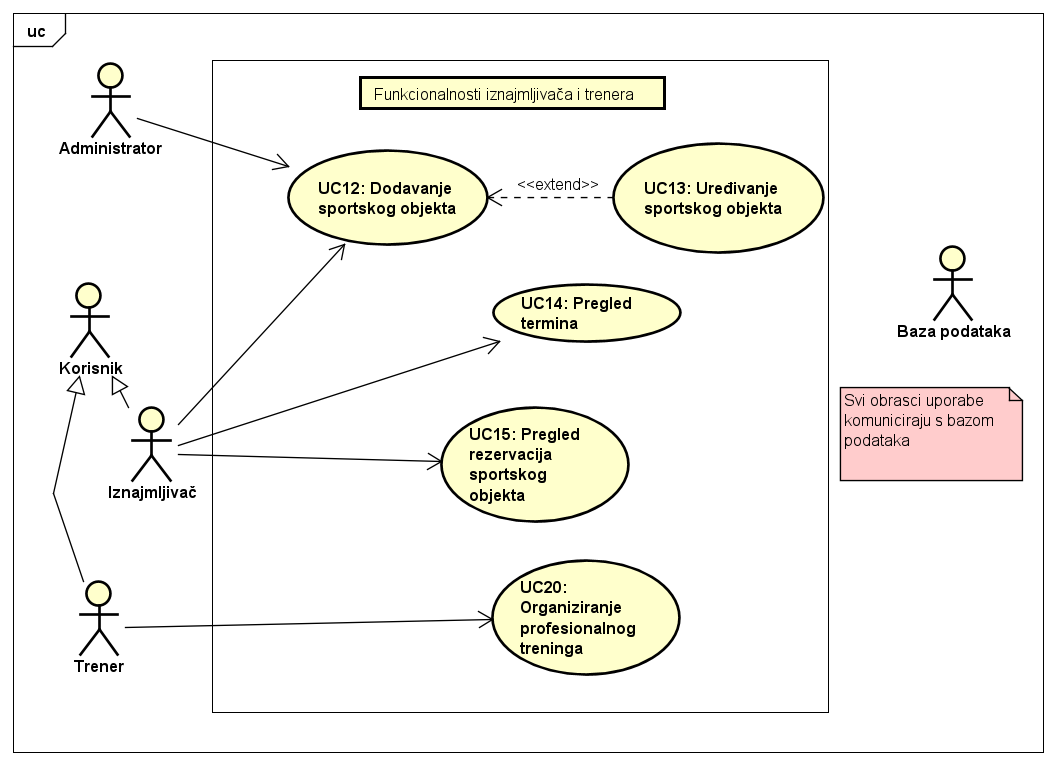
\includegraphics[width=1\linewidth]{slike/IznajmljivacTrener.PNG}
						\centering
						\caption{Funkcionalnosti iznajmljivača i trenera}
						\label{fig:funkcionalnosti_iznajmljivac_trener}
					\end{figure}
					\begin{figure}[H]
						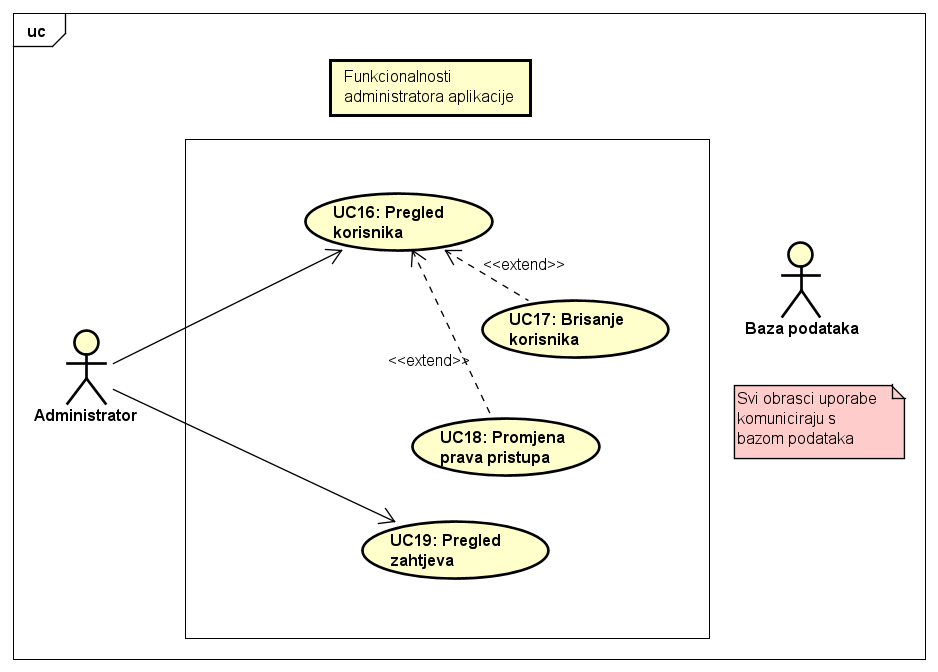
\includegraphics[width=1\linewidth]{slike/Administrator.PNG}
						\centering
						\caption{Funkcionalnosti administratora aplikacije}
						\label{fig:funkcionalnosti_administrator}
					\end{figure}
				\eject		
				
			\subsection{Sekvencijski dijagrami}
				
				\begin{comment}
				\textbf{\textit{dio 1. revizije}}\\
				
				\textit{Nacrtati sekvencijske dijagrame koji modeliraju najvažnije dijelove sustava (max. 4 dijagrama). Ukoliko postoji nedoumica oko odabira, razjasniti s asistentom. Uz svaki dijagram napisati detaljni opis dijagrama.}
				\eject
				\end{comment}
				
				\subsubsection{Obrazac uporabe UC6 - Promjena osobnih podataka}
				Prijavljeni korisnik šalje zahtjev za promjenu podataka. Poslužitelj zatim prikazuje korisnikove trenutne podatke i omogućuje mu izmjenu. Zatim korisnik unosi nove podatke te potvrđuje promjenu. Ako je korisnik ispravno unio podatke, poslužitelj sprema osvježene podatke u bazu podataka. Nakon što poslužitelj dobije potvrdu od baze da su podaci spremljeni, šalje korisniku obavijest da su novi podaci spremljeni u sustav. Ako je korisnik neispravno unio podatke, poslužitelj ga odmah obaviještava o neispravnosti podataka.
				
				\begin{figure}[H]
					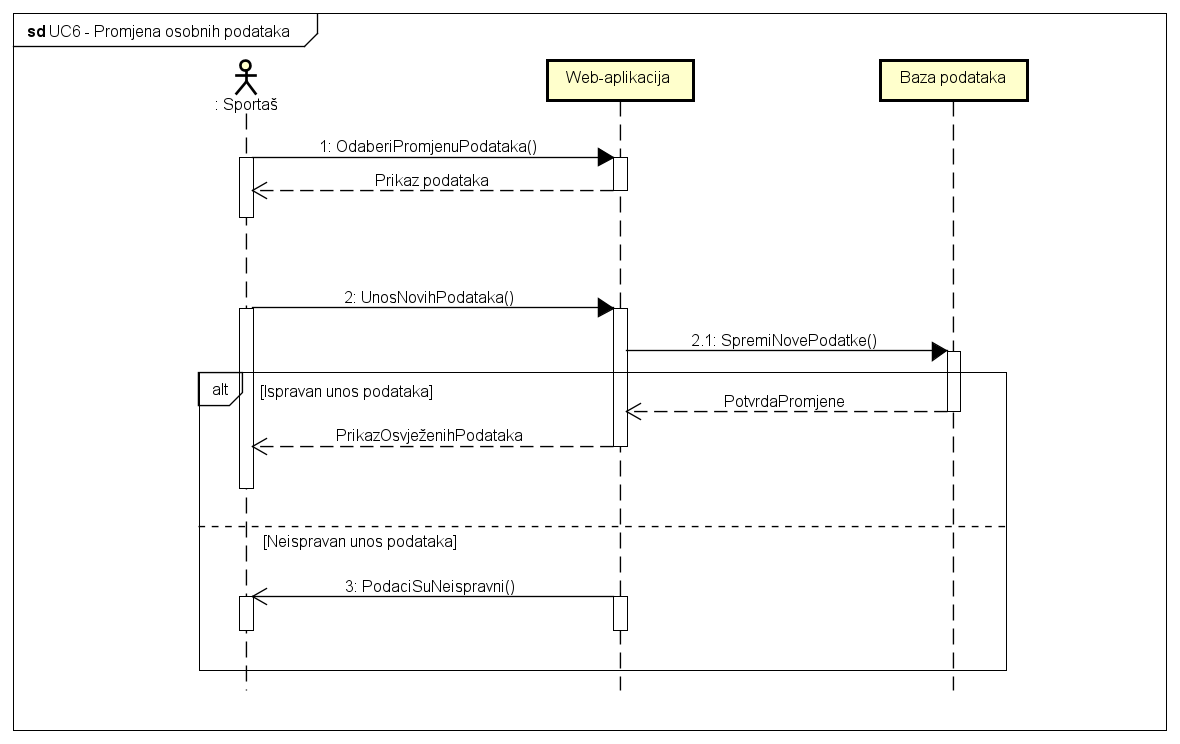
\includegraphics[width=\textwidth]{slike/UC6_SEKV_DIJ.png}
					\caption{Sekvencijski dijagram za UC6}
				\end{figure}
			
				\subsubsection{Obrazac uporabe UC7 - Prijava na sportsku aktivnost}
				Prijavljeni korisnik šalje zahtjev za odabir željene sportske aktivnosti. Poslužitelj zatim prikazuje kartu na kojoj se nalaze sve lokacije na kojima se održava sportska aktivnost koju je korisnik odabrao i koje imaju slobodnih mjesta. Korisnik zatim odabire željenu lokaciju i prijavljuje se za aktivnost. Poslužitelj zatim sprema prijavu u bazu podataka. Nakon što poslužitelj dobije potvrdu od baze da su podaci spremljeni, preusmjerava korisnika na stranicu gdje se nalaze sve prijavljene korisnikove aktivnosti. 
				
				\begin{figure}[H]
					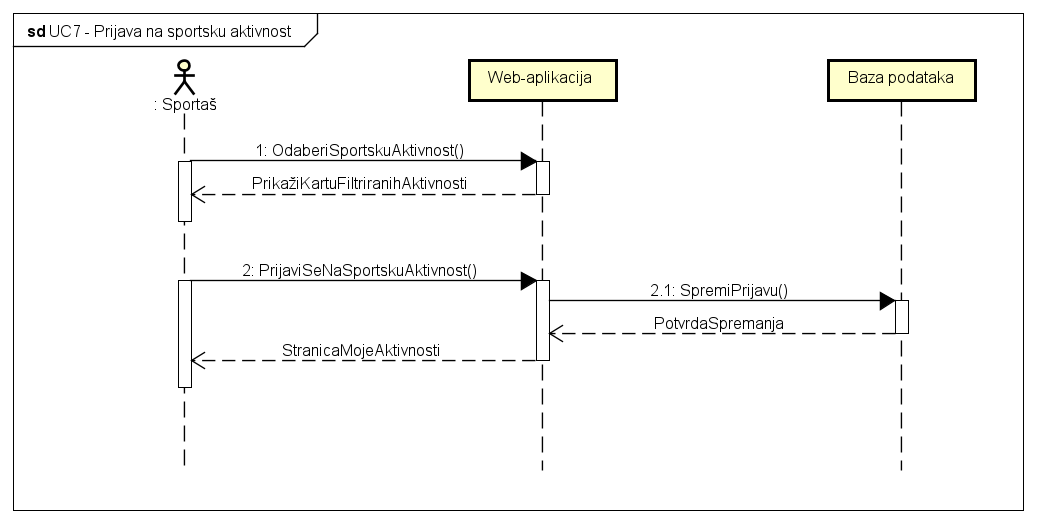
\includegraphics[width=\textwidth]{slike/UC7_SEKV_DIJ.png}
					\caption{Sekvencijski dijagram za UC7}
				\end{figure}
			
				\subsubsection{Obrazac uporabe UC10 - Iznajmljivanje sportskih površina/dvorana}
				Prilikom organiziranja sportske aktivnosti prijavljeni korisnik šalje zahtjev za iznajmljivanje sportske površine/dvorane. Poslužitelj zatim prikazuje dostupne sportske površina/dvorana koje se mogu iznajmiti. Prijavljeni korisnik zatim odabire željenu sportsku površinu/dvoranu. Nakon toga prijavljeni korisnik odabire željeni datum. Poslužitelj zatim provjerava u bazi postoje li slobodni termini na datum koji je korisnik izabrao. Ako oni ne postoje, obaviještava se korisnika da odabere neki drugi datum. Ako postoje slobodni termini na odabrani datum poslužitelj ih prikazuje prijavljenom korisniku. Korisnik zatim odabire željeni termin i nakon toga šalje zahtjev za potvrdu rezervacije. Poslužitelj sprema rezervaciju u bazu podataka i nakon što dobije potvrdu da je rezervacija spremljena o tome obaviještava korisnika.
				
				\begin{figure}[H]
					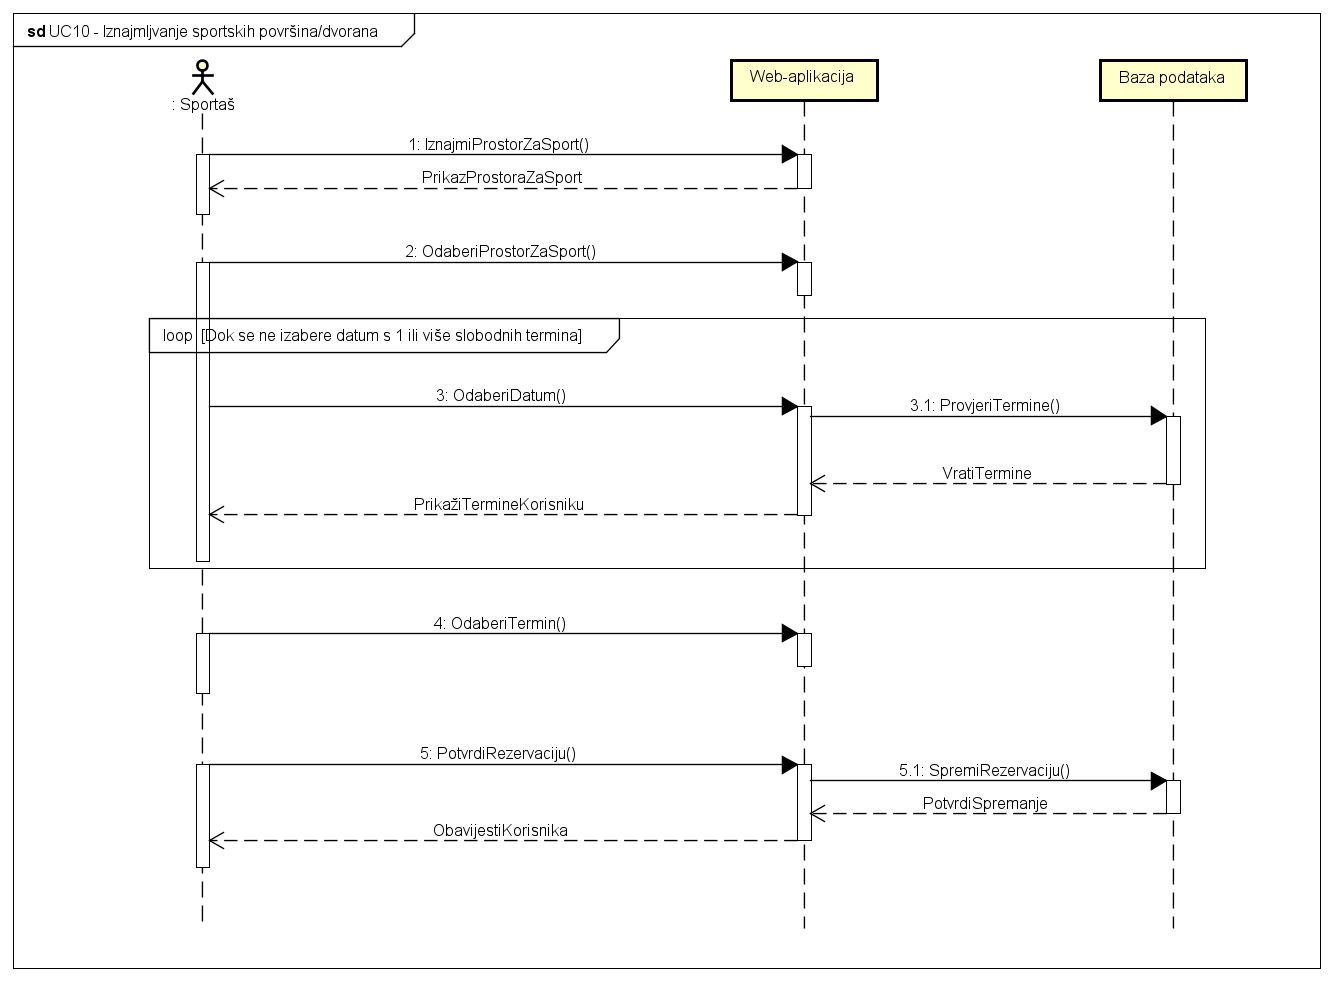
\includegraphics[width=\textwidth]{slike/UC10_SEKV_DIJ.png}
					\caption{Sekvencijski dijagram za UC10}
				\end{figure}
			
				\subsubsection{Obrazac uporabe UC21 - Prilaganje službene dokumentacije}
				Prijavljeni korisnik šalje zahtjev za dodavanje službene dokumentacije. Poslužitelj prikazuje obrazac za prijavu dokumentacije. Prijavljeni korisnik zatim unosi svoje podatke, te ako su oni ispravni poslužitelj ih sprema u bazu podataka. Nakon što baza podataka spremi podatke, vraća potvrdu poslužitelju koji zatim preusmjerava prijavljenog korisnika na stranicu kojom se korisniku daje do znanja da je njegova prijava zaprimljena te da će biti obaviješten kada ona bude obrađena. Administrator zatim može zatražiti pregled svih dokumentacija iz baze podataka i pregledati nove prijave. Ako su svi podaci ispravni administrator potvrđuje dokumentaciju i potvrđenu dokumentaciju sprema u bazu podataka. Ako su podaci neispravni prijava se briše iz baze podataka. Zatim administrator osvježi stanje prijave na poslužitelju, a nakon toga poslužitelj obaviještava korisnika o stanju njegove prijave. Ako su podaci bili neispravni kod samog upisa poslužitelj odmah javlja grešku korisniku.
				
				\begin{figure}[H]
					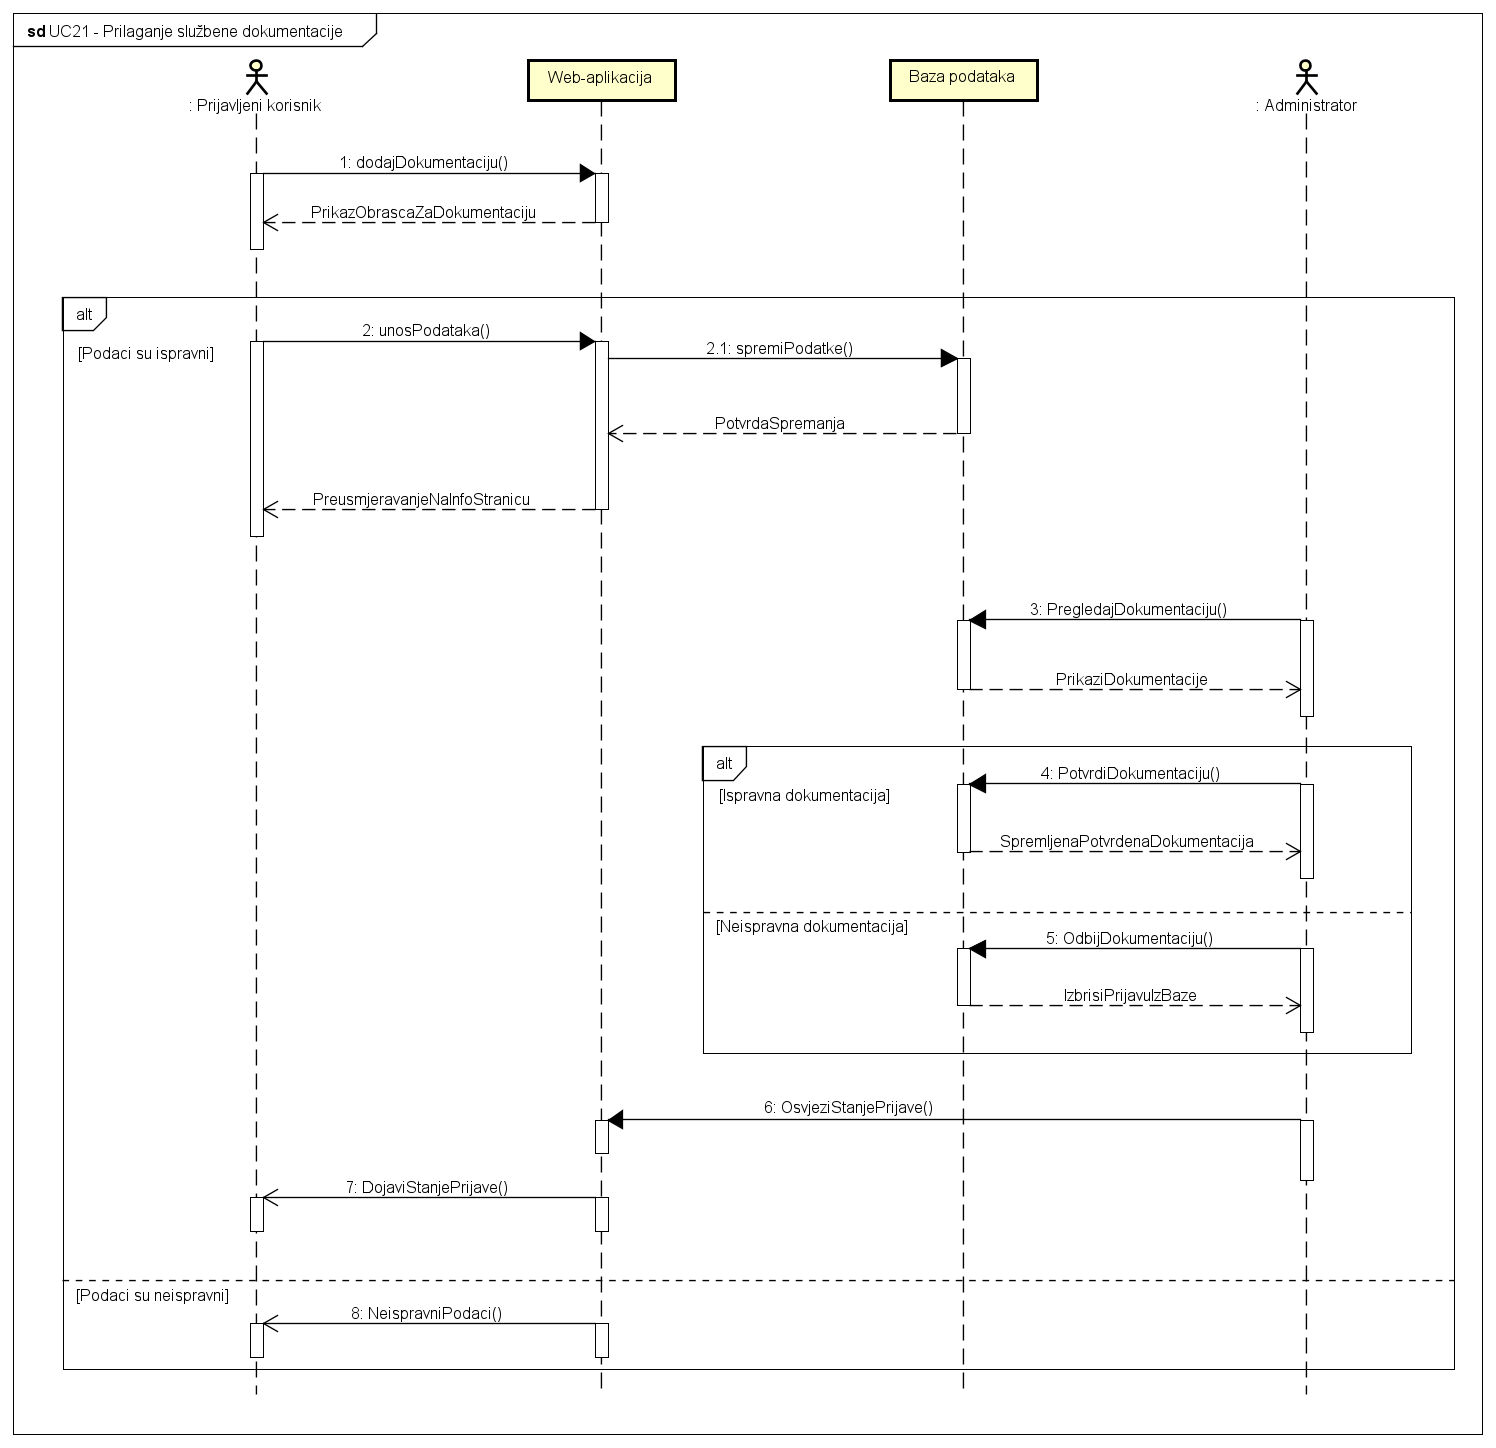
\includegraphics[width=\textwidth]{slike/UC21_SEKV_DIJ.png}
					\caption{Sekvencijski dijagram za UC21 }
				\end{figure}
		\eject
		\section{Ostali zahtjevi}
		
			\begin{comment}
			\textbf{\textit{dio 1. revizije}}\\
		 
			 \textit{Nefunkcionalni zahtjevi i zahtjevi domene primjene dopunjuju funkcionalne zahtjeve. Oni opisuju \textbf{kako se sustav treba ponašati} i koja \textbf{ograničenja} treba poštivati (performanse, korisničko iskustvo, pouzdanost, standardi kvalitete, sigurnost...). Primjeri takvih zahtjeva u Vašem projektu mogu biti: podržani jezici korisničkog sučelja, vrijeme odziva, najveći mogući podržani broj korisnika, podržane web/mobilne platforme, razina zaštite (protokoli komunikacije, kriptiranje...)... Svaki takav zahtjev potrebno je navesti u jednoj ili dvije rečenice.}
			\end{comment}
			
			\begin{itemize}
				\setlength{\itemsep}{0pt}
				\setlength{\parskip}{0pt}
				\item Sustav treba biti implementiran kao web aplikacija koristeći objektno-orijentirane jezike
				\item Pristup bazi podataka mora biti zaštićen i ne smije trajati duže od nekoliko sekundi
				\item Sustav mora podržavati hrvatsku abecedu uključujući dijakritičke znakove
				\item Sustavu istovremeno mogu pristupiti više različitih vrsta korisnika
				\item Korisničko sučelje mora biti jednostavno, responzivno i intuitivno za korištenje te se mora ispravno prikazivati na stolnim računalima, laptopima i mobilnim uređajima
				\item Neispravno korištenje korisničkog sučelja ne smije narušiti funkcionalnosti sustava
				\item Nadogradnja sustava ne smije narušiti funkcionalnosti sustava
				\item Sustav mora prijavljenim korisnicima jasno prikazati ovlasti koje im pripadaju (sportaš, trener, iznajmljivač)
				\item Sustav kao valutu za prikaz cijena i transakcija koristi HRK
				\item Pristup sustavu se mora odvijati pomoću protokola HTTPS
			\end{itemize}
			
			 
			 
			 
	
	\chapter{Arhitektura i dizajn sustava}
		
		Oblikovanje arhitekture i dizajna sustava jedno je od temeljnih i najvažnijih faza razvoja programske potpore. Uključuje glavna pravila i strukture sustava te se sve dalje izgrađuje na osnovi te arhitekture. Upravo zbog toga je ključan faktor u uspješnosti projekta, cijeni i težini izrade te održavanja. 
		
		Za našu aplikaciju odabrali smo objektno orijentiranu arhitekturu jer se pokazala kao najprikladnija za kompleksnu više-korisničku aplikaciju. Kako bi cilj omogućavanja što lakšeg i šireg korištenja naše aplikacije bio ispunjen, odabrali smo izradu web aplikacije kojoj će korisnici moći pristupiti s bilo kojeg uređaja s web preglednikom i  spojenim na mrežu.
		
		Na slici su vidljivi podsustavi klijent-poslužitelj arhitekture sustava. Komunikacija između web preglednika i web poslužitelja odvija se putem HTTP protokola.
	
		\begin{figure}[H]
			\centering
			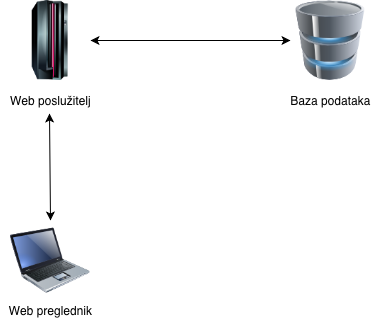
\includegraphics[scale=0.4]{slike/ArhSustav.png}
			\caption{Arhitektura sustava}
		\end{figure}

		\underline{Web preglednik} je program putem kojega korisnik pristupa web-aplikaciji, šalje zahtjeve web poslužitelju i prikazuje vizualnu interpretaciju odgovora.
		
		\underline{Web poslužitelj} prima zahtjeve od korisnika i prosljeđuje ih web aplikaciji koja je pokrenuta na njemu, a odgovore na taj zahtjev, koje dobije od web aplikacije, prosljeđuje natrag web pregledniku korisnika.
		
		\underline{Web aplikacija} na osnovu logike sustava, zahtjeva korisnika i podataka iz baze podataka generira odgovor na zahtjev korisnika.
		
		Objektno orijentirana paradigma je način modeliranja sustava u kojem su osnova izgradnje objekti i modularnost, a osnovni elementi su:
		
			\begin{packed_item}
			
			\item \textbf{Objekt }- primjerak razreda, odnosno smislene cjeline, sadrži vlastite atribute i metode
			\item \textbf {Nasljeđivanje }- mogućnost preuzimanja metoda od razreda-roditelja ili nadjačavanje istih vlastitim proširenjima
			\item \textbf{Polimorfizam }- moguće je postojanje metoda istog imena, a različitih atributa i funkcionalnosti 
			\end{packed_item}
		
		Oblikovanje navedene arhitekture pratit će MVC(Model-View-Controller) obrazac koji se sastoji od:
		
			\begin{packed_item}
				\item \textbf{Model }- struktura za spremanje i upravljanje objektima i podacima
				\item \textbf{View }- komponenta za vizualni prikaz podataka korisniku
				\item \textbf{Controller }- sadrži logiku upravljanja korisničkim zahtjevima i na osnovu nje prilagođava podatke iz modela i prosljeđuje ili preusmjerava View-u za prikaz 
			\end{packed_item}
		
		\begin{figure}[H]
			\centering
			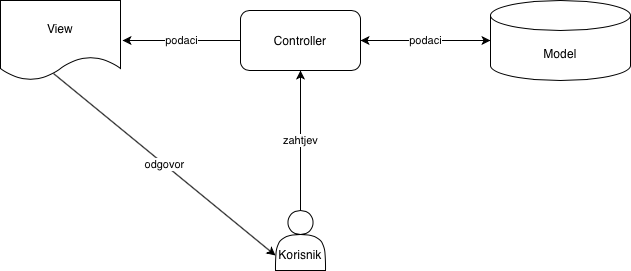
\includegraphics[scale=0.5]{slike/mvc.png}
			\caption{Arhitektura sustava}
		\end{figure}
	
		Praćenje MVC obrasca omogućuje razdvajanje ovisnosti i odgovornosti što rezultira u olakšanju paralelnog razvoja više dijelova aplikacije, testiranju i naknadnom dodavanju funkcionalnosti u sustav.
		
		Arhitektura sustava iz pogleda aktora sadrži sljedeće podsustave:
		
		\begin{packed_item}
			\item Aplikacija za sportaše i trenere
			\item Aplikacija za iznajmljivače
			\item Aplikacija za administratora
		\end{packed_item}
		
		Implementacijski je arhitektura podijeljena na backend i frontend.
		Frontend obuhvaća komponente vezane za vizualni prikaz kranjem korisniku i baziran je na \clickablefootnotelink{React-u}{https://reactjs.org/}, open-source Javascript biblioteci. Backend sloj izravno prati MVC razvojni obrazac i za njega je korišten programski jezik Java, točnije Spring okvir, kojemu je jedna od glavnih značajki inverzija ovisnosti. Osim toga nudi i gotove implementacije mnogobrojnih protokola i automatsko namještanje detaljnih postavki sustava. Za sigurnost je korišten JWT (JSON Web Token) koji je popularni otvoreni standard tokena za potpisivanje i enkripciju prilikom slanja podataka u JSON formatu.

				
		\section{Baza podataka}
			
		Kako bi se korisniku omogućila brza i efikasna izmjena i pregled podataka web aplikacija je u interakciji s bazom podataka. Baza zadovoljava treću normalnu formu te se brine o konzistentnosti podataka, primarnim i stranim ključevima te integritetskim ograničenjima. Baza se brine o istodobnom pristupu podacima, dakle transakcije zadovoljavaju svojstva ACID(Atomicity, Consistency, Isolation, Durability). Za upravljanje bazom podataka koristimo sustav PostgreSql zbog toga što je to besplatan sustav te je otvorenog koda i dostupan je za više operacijskih sustava.
		
			\subsection{Opis tablica}
			
			U nastavku navedeni su entiteti i atributi koje sadrži baza podataka te njihov tip podatka i opis. Atributi koji su u tablici označeni svijetlozelenom bojom predstavljaju primarni ključ, a atributi označeni svijetloplavom su strani ključevi.\\\\
				\begin{longtabu} to \textwidth {|X[6, l]|X[6, l]|X[20, l]|}
					\hline \multicolumn{3}{|c|}{\textbf{t\_user}}	 \\[3pt] \hline
					\endfirsthead
					\hline \multicolumn{3}{|c|}{\textbf{t\_user}}	 \\[3pt] \hline
					\endhead
					
					\hline 
					\endlastfoot
					
					\hline
					\cellcolor{LightGreen}id & INT	&  	Jedinstveni identifikator svakog korisnika registriranog u sustavu. 	\\ \hline
					username	 & VARCHAR & Korisničko ime s kojime se korisnik prijavljuje u sustav.  	\\ \hline 
					passwd\_hash & VARCHAR & Zaporka u obliku sažetka(hasha).  \\ \hline
				\end{longtabu}
				U relaciji t\_user nalaze se korisničko ime, zaporka te id koji služi kao jedinstveni identifikator svakog korisnika prijavljenog u sustav.
				
				
				\begin{longtabu} to \textwidth {|X[6, l]|X[6, l]|X[20, l]|}
					\hline \multicolumn{3}{|c|}{\textbf{t\_administrator}}	 \\[3pt] \hline
					\endfirsthead
					\hline \multicolumn{3}{|c|}{\textbf{t\_adminstrator}}	 \\[3pt] \hline
					\endhead
					
					\hline 
					\endlastfoot
					
					\hline
					\cellcolor{LightGreen}id & INT & Identifikator Jedinstveni identifikator svakog korisnika registriranog u sustav. \\ \hline
				\end{longtabu}
				Relacija t\_administrator sadrži identifikatore svih registriranih korisnika koji rade kao administratori sustava i imaju posebne ovlasti. Administrator odobrava i provjerava istinitost podataka i dokumenata koje prilažu iznajmljivači i treneri.  Id je strani ključ koji se poziva na relaciju t\_users. \\



				\begin{longtabu} to \textwidth {|X[6, l]|X[6, l]|X[20, l]|}
					\hline \multicolumn{3}{|c|}{\textbf{t\_person}}	 \\[3pt] \hline
					\endfirsthead
					\hline \multicolumn{3}{|c|}{\textbf{t\_person}}	 \\[3pt] \hline
					\endhead
					\hline 
					\endlastfoot
					\hline
					\cellcolor{LightGreen}id & INT	&  	Jedinstveni identifikator svakog korisnika registriranog u sustavu.\\ \hline
					email & VARCHAR & Email adresa sa kojom je povezan korisnički račun.  	\\ \hline
					name & VARCHAR & Korisnikovo ime.  	\\ \hline
					surname & VARCHAR & Korisnikovo prezime.  	\\ \hline 
					
				\end{longtabu}
				Relacija t\_person odnosi se na sve korisnike koji su registrirani kao sportaši, iznajmljivači ili treneri. Za njih bilježimo email ime i prezime. U relaciji tajođer postoji id kao strani ključ koji se poziva na relaciju t\_user. \\
				
				
				\begin{longtabu} to \textwidth {|X[6, l]|X[6, l]|X[20, l]|}
					\hline \multicolumn{3}{|c|}{\textbf{t\_athlete}}	 \\[3pt] \hline
					\endfirsthead
					\hline \multicolumn{3}{|c|}{\textbf{t\_person}}	 \\[3pt] \hline
					\endhead
					\hline 
					\endlastfoot
					\hline
					\cellcolor{LightGreen}id & INT	&  	Jedinstveni identifikator svakog korisnika registriranog u sustavu.\\ \hline
					birthday\_date\_date & TIMESTAMP & Datum rođernja sportaša.  	\\ \hline
					gender & VARCHAR & Spol sportaša.  	\\ \hline
					height & DOUBLE & Sportaševa visina izražena u cm.  	\\ \hline 
					weight & VARCHAR & Sportaševa težina izražena u kg.  \\ \hline
					
				\end{longtabu}
				Relacija t\_athlete sadrži sve bitne podatke o korisnicima koji se u sustav prijavljuju kao sportaši. Sportaši su korisnici koji se mogu prijaviti ili organizirazi sportska okupljanja odnosno događaje koji se ne naplaćuju i nisu pod profesionalnim vodstvom. U relaciji tajođer postoji id kao strani ključ koji se poziva na relaciju t\_users. \\
				
				
				\begin{longtabu} to \textwidth {|X[6, l]|X[6, l]|X[20, l]|}
					\hline \multicolumn{3}{|c|}{\textbf{t\_renter}}	 \\[3pt] \hline
					\endfirsthead
					\hline \multicolumn{3}{|c|}{\textbf{t\_renter}}	 \\[3pt] \hline
					\endhead
					\hline 
					\endlastfoot
					\hline
					\cellcolor{LightGreen}id & INT & Identifikator Jedinstveni identifikator svakog korisnika registriranog u sustav. \\ \hline
				\end{longtabu}
				Relacija t\_renter sadrži identifikatore svih registriranih korisnika koji su se u sustav prijavili kao iznajmljivači sportskih objekata. Oni u sustav mogu dodati svoj sportski objekt navodeći njegove specifikacije poput lokacije, tipa sportova koji se u tom objektu mogu igrati, cijene po satu i termine dostupne za rezervaciju. Id je strani ključ koji se poziva na relaciju t\_user. \\			
				
				
				
				
				\begin{longtabu} to \textwidth {|X[6, l]|X[6, l]|X[20, l]|}
					\hline \multicolumn{3}{|c|}{\textbf{t\_coach}}	 \\[3pt] \hline
					\endfirsthead
					\hline \multicolumn{3}{|c|}{\textbf{t\_coach}}	 \\[3pt] \hline
					\endhead
					\hline 
					\endlastfoot
					\hline
					\cellcolor{LightGreen}id & INT & Identifikator Jedinstveni identifikator svakog korisnika registriranog u sustav. \\ \hline
				\end{longtabu}
				Relacija t\_coach sadrži identifikatore svih trenera. Za razliku od sportaša treneri mogu organizirati i treninge  za koje mogu postaviti određenu cijenu. \\
				
				
				
				\begin{longtabu} to \textwidth {|X[6, l]|X[6, l]|X[20, l]|}
					\hline \multicolumn{3}{|c|}{\textbf{t\_location}}	 \\[3pt] \hline
					\endfirsthead
					\hline \multicolumn{3}{|c|}{\textbf{t\_location}}	 \\[3pt] \hline
					\endhead
					\hline 
					\endlastfoot
					\hline
					\cellcolor{LightGreen}id & INT & Jedinstveni identifikator svake lokacije dostupne u sustavu. \\ \hline
					 name & VARCHAR & Naziv lokacije.	\\ \hline
					 location\_type & VARCHAR &  Javna površina ili plaćeni sportski objekt.	\\ \hline
					 gpxcoordinates & VARCHAR & Geografske kordinate lokacije.	\\ \hline
					 \cellcolor{LightBlue}person\_id & INT & Identifikator korisnika koji je sportsku lokaciju dodao u sustav.\\
					 
				\end{longtabu}
				U relacijai t\_location nalaze sve sve lokacije unesene u sustav. Ovisno o tipu lokacije razlikujemo plaćene i javno dostupne lokacije. Za lokacije bilježi se id kreatora lokacije odnosno korisnika koji je unjeo u sustav lokaciju i potrebne podatke. Plaćene lokacije dopušteno je kreiraiti samo korisnicima kojima je odobren status iznajmljivača. Za plaćene lokacije evidentira se id iznajmljivača koji posjeduju taj objekt. Također u relaciji se spremaju kordinate lokacije koje mogu poslužiti kao marker na karti u slučaju jedne kordinate ili za iscrtavanje cijelog poligona u slučaju više zabilježenih koordinata.  \\
				
				
				
				\begin{longtabu} to \textwidth {|X[6, l]|X[6, l]|X[20, l]|}
					\hline \multicolumn{3}{|c|}{\textbf{t\_opening}}	 \\[3pt] \hline
					\endfirsthead
					\hline \multicolumn{3}{|c|}{\textbf{t\_opening}}	 \\[3pt] \hline
					\endhead
					\hline 
					\endlastfoot
					\hline
					\cellcolor{LightGreen}id & INT & Jedinstveni identifikator radnog vremena.	\\ 
					\hline
					cost & DOUBLE & Cijena u slučaju plaćene lokacije.	\\ \hline
					start\_time & TIME & Vrijeme otvaranja.	\\ \hline
					end\_time & TIME & Vrijeme zatvaranja.	\\ \hline
					from\_date & TIMESTAMP & Datum početka rasporeda.	\\ \hline
					to\_date & TIMESTAMP & Datum kraja rasporeda.	\\ \hline
					weekday & INT & Dan u tjednu na kojega se odnosi radno vrijeme.	\\ \hline
				\end{longtabu}
				Relacija t\_opening evidentiraju se radna vremena koja možemo pridružiti nkeim lokacijama. Za radno vrijeme evidentiraju se početak i kraj te u kojemu danu te datumi odkada dokada se takav raspred proteže. \\
				
				
				
				\begin{longtabu} to \textwidth {|X[6, l]|X[6, l]|X[20, l]|}
					\hline \multicolumn{3}{|c|}{\textbf{t\_location\_openings}}	 \\[3pt] \hline
					\endfirsthead
					\hline \multicolumn{3}{|c|}{\textbf{t\_location\_openings}}	 \\[3pt] \hline
					\endhead
					\hline 
					\endlastfoot
					\hline
					\cellcolor{LightGreen}paid\_location-\_id & INT & Identifikator lokacije za iznajmljivanje.	\\ \hline
					\cellcolor{LightGreen} openings\_id & INT & Identifikator radnog vremena iz realcije t\_opening.	\\ \hline
				\end{longtabu}
				Relacija t\_location\_open\_hours služi kao veza između relacija t\_opening i t\_location. U njoj su evidentirani radna vremena za sve plaćene lokacije.\\
				
				
				
				\begin{longtabu} to \textwidth {|X[6, l]|X[6, l]|X[20, l]|}
					\hline \multicolumn{3}{|c|}{\textbf{t\_sport}}	 \\[3pt] \hline
					\endfirsthead
					\hline \multicolumn{3}{|c|}{\textbf{t\_sport}}	 \\[3pt] \hline
					\endhead
					\hline 
					\endlastfoot
					\cellcolor{LightGreen}id & INT & Jedinstveni identifikator pojedinog sporta.	\\ \hline
					name & VARCHAR & Naziv sporta.	\\ \hline
					iconbwuri & VARCHAR & URI crno bijele ikone.	\\ \hline
					icon\_color\_uri & VARCHAR & URI ikone s bojom.	\\ \hline
					type & VARCHAR & Tip sporta (indoor/outdoor).	\\ \hline
				\end{longtabu}
				U relaciji t\_sport nalazi se popis svih sportova evidentiranih u sustavu. Svaki sport ima id, ime i tip u ovisnosti o tome igra li se sport u zatvorenom prostoru ili ne. \\
				
				
				\begin{longtabu} to \textwidth {|X[6, l]|X[6, l]|X[20, l]|}
					\hline \multicolumn{3}{|c|}{\textbf{t\_sportevent}}	 \\[3pt] \hline
					\endfirsthead
					\hline \multicolumn{3}{|c|}{\textbf{t\_sportevent}}	 \\[3pt] \hline
					\endhead
					\hline 
					\endlastfoot
					\cellcolor{LightGreen}id & INT & Jedinstveni identifikator svakog sportskog eventa.	\\ \hline
					\cellcolor{LightBlue} location\_id & INT & Jedinstveni identifikator lokacije na kojoj se održava sportski event.	\\ \hline
					\cellcolor{LightBlue} organizer\_id & INT & Jedinstveni identifikator organizatora sportskog eventa.	\\ \hline
					\cellcolor{LightBlue} sport\_id & INT & Jedinstveni identifikator sporta koji se igra na eventu.	\\ \hline
					sportevent-\_type & VARCHAR & Plaćeni ili neplaćeni event (amateur/professional).	\\ \hline
					max\_number-\_of\_participants & INT & Broj koliko ljudi maksimalno može sudjelovati na sportskom eventu.	\\ \hline
					start\_date\_time & TIMESTAMP & Datum i sat početka eventa.	\\ \hline
					end\_date\_time & TIMESTAMP & Datum i sat kraja eventa.	\\ \hline
					cost & DOUBLE & Cijena prisustvovanja u slučaju plaćenih eventova.	\\ \hline
					
				\end{longtabu}
				U relaciji t\_sportevent vidi se popis svih organiziranih sportskih eventova. Razlikujemo amaterskke i profesionalne eventove po tome plaćaju li se ili ne odnosno tko ih je organizirao trener ili sportaš. Za svaki event unesen u sustav poznat nam je datum i vrijeme početka i kraja eventa, maksimalan broj sudionika, cijena, koji sport se može igrati, tko je organizirao event i naravno na kojoj lokaciji će se event održavati.   \\
				
				
				
				\begin{longtabu} to \textwidth {|X[6, l]|X[6, l]|X[20, l]|}
					\hline \multicolumn{3}{|c|}{\textbf{t\_sportevent\_participants}}	 \\[3pt] \hline
					\endfirsthead
					\hline \multicolumn{3}{|c|}{\textbf{t\_sportevent\_participants}}	 \\[3pt] \hline
					\endhead
					\hline 
					\endlastfoot
					\cellcolor{LightGreen} events\_participation\_id & INT & Identifikator sportskog eventa u kojemu korisnik prisustvuje.	\\ \hline
					\cellcolor{LightGreen} participants\_id & INT & Identifikator korisnika koji prisustvuje u eventu.	\\ \hline
				\end{longtabu}
				U relaciji t\_sportevent\_participants evidentiramo id svakog korisnika koji prisustvuje u nekom eventu te id eventa u kojem prisustvuje.\\
				
				
				
				
				\begin{longtabu} to \textwidth {|X[6, l]|X[6, l]|X[20, l]|}
					\hline \multicolumn{3}{|c|}{\textbf{t\_documentation}}	 \\[3pt] \hline
					\endfirsthead
					\hline \multicolumn{3}{|c|}{\textbf{t\_documentation}}	 \\[3pt] \hline
					\endhead
					\hline 
					\endlastfoot
					
					\cellcolor{LightGreen}id & INT & Jedinstveni identifikator dokumenta.	\\ \hline
					document-\_intern\_uri & VARCHAR & Uri dokumenta.	\\ \hline
					type & INT & Vrsta dokumenta.	\\ \hline
					\cellcolor{LightBlue} approved\_by\_id & INT & Identifikator administratora koji je potvrdio dokument.	\\ \hline
				\end{longtabu}
				U relaciji t\_documentation nalazi se popis svih dokumenata koje prilažu sportaši koji žele postati treneri i iznajmljivači da bi im se priznao status iznajmljivača. Također evidentira se koji administrator potvrđuje ili odbacuje dokumentaciju. \\
				
				
				\begin{longtabu} to \textwidth {|X[6, l]|X[6, l]|X[20, l]|}
					\hline \multicolumn{3}{|c|}{\textbf{t\_coach\_coach\_certificate}}	 \\[3pt] \hline
					\endfirsthead
					\hline \multicolumn{3}{|c|}{\textbf{t\_coach\_coach\_certificate}}	 \\[3pt] \hline
					\endhead
					\hline 
					\endlastfoot
					
					\cellcolor{LightGreen}coach\_id & INT & Jedinstveni identifikator trenera.	\\ \hline
					\cellcolor{LightGreen} coach-\_certificate\_id & INT & Id dokumenta (certifikata trenera).	\\ \hline
				\end{longtabu}
				Relacija t\_coach\_coach\_certificate sadrži parove identifikatora trenera i identifikatora dokumenta koje prilažu da bi potvrdili svoj status trenera.  \\
				
				
				
				\begin{longtabu} to \textwidth {|X[6, l]|X[6, l]|X[20, l]|}
					\hline \multicolumn{3}{|c|}{\textbf{t\_location\_ownership\_certificate}}	 \\[3pt] \hline
					\endfirsthead
					\hline \multicolumn{3}{|c|}{\textbf{t\_location\_ownership\_certificate}}	 \\[3pt] \hline
					\endhead
					\hline 
					\endlastfoot
	
					\cellcolor{LightGreen}paid\_location-\_id & INT & Jedinstveni identifikator lokacije.	\\ \hline
					\cellcolor{LightGreen} ownership-\_certificate\_id & INT & Identifikator dokumenta.	\\ \hline
				\end{longtabu}
				Relacija t\_location\_ownership\_certificate sadrži parove identifikatora iznajmljivača i identifikatora dokumenta kojeg prilažu da bi dokazali da posjeduju sportski objekt kojeg žele iznajmljivati.  \\
				
				
				\begin{longtabu} to \textwidth {|X[6, l]|X[6, l]|X[20, l]|}
					\hline \multicolumn{3}{|c|}{\textbf{t\_documentation\_sports}}	 \\[3pt] \hline
					\endfirsthead
					\hline \multicolumn{3}{|c|}{\textbf{t\_documentation\_sports}}	 \\[3pt] \hline
					\endhead
					\hline 
					\endlastfoot
					
					\cellcolor{LightGreen}documentation-\_id & INT & Jedinstveni identifikator dokumenta.	\\ \hline
					\cellcolor{LightGreen} sports\_id & INT & Identifikator sporta.	\\ \hline
				\end{longtabu}
				Relacija t\_documentation\_sports sadrži parove identifikatora dokumenta koje trener prilaže da mu se potvrdi status trenera i identifikatora sporta na koji se taj dokument odnosi.  \\
				
				
				
				\begin{longtabu} to \textwidth {|X[6, l]|X[6, l]|X[20, l]|}
					\hline \multicolumn{3}{|c|}{\textbf{t\_location\_available\_sports}}	 \\[3pt] \hline
					\endfirsthead
					\hline \multicolumn{3}{|c|}{\textbf{t\_location\_available\_sports}}	 \\[3pt] \hline
					\endhead
					\hline 
					\endlastfoot
					
					\cellcolor{LightGreen} location\_id & INT & Jedinstveni identifikator lokacije.	\\ \hline
					\cellcolor{LightGreen} available-\_sports\_id & INT & Identifikator sporta.	\\ \hline
				\end{longtabu}
				Relacija t\_location\_available\_sports sadrži parove identifikatora lokacije i sportova koji se mogu igrati na toj lokaciji.  \\
				
				
				\begin{longtabu} to \textwidth {|X[6, l]|X[6, l]|X[20, l]|}
					\hline \multicolumn{3}{|c|}{\textbf{t\_sportevent\_location\_reservation\_inquery}}	 \\[3pt] \hline
					\endfirsthead
					\hline \multicolumn{3}{|c|}{\textbf{t\_sportevent\_location\_reservation\_inquery}}	 \\[3pt] \hline
					\endhead
					\hline 
					\endlastfoot
					
					\cellcolor{LightGreen} reservation-\_queue\_id & INT & Jedinstveni identifikator liste za čekanje.	\\ \hline
					\cellcolor{LightGreen} location-\_reservation-\_inquery\_id & INT & Identifikator rezervacije.	\\ \hline
				\end{longtabu}
				Relacija t\_sportevent\_location\_reservation\_inquery Sadrži podatke o rezervaciji lokacije za sportska događanja.  \\
				
				
				
				
				

	
			
		\newgeometry{left=0.5cm,bottom=0.5cm,right=0.5cm,top=0.5cm}
		\begin{landscape}
			
			\section{Dijagram baze podataka}
			\thispagestyle{empty}
			\begin{figure}[ht!]
				\centering
				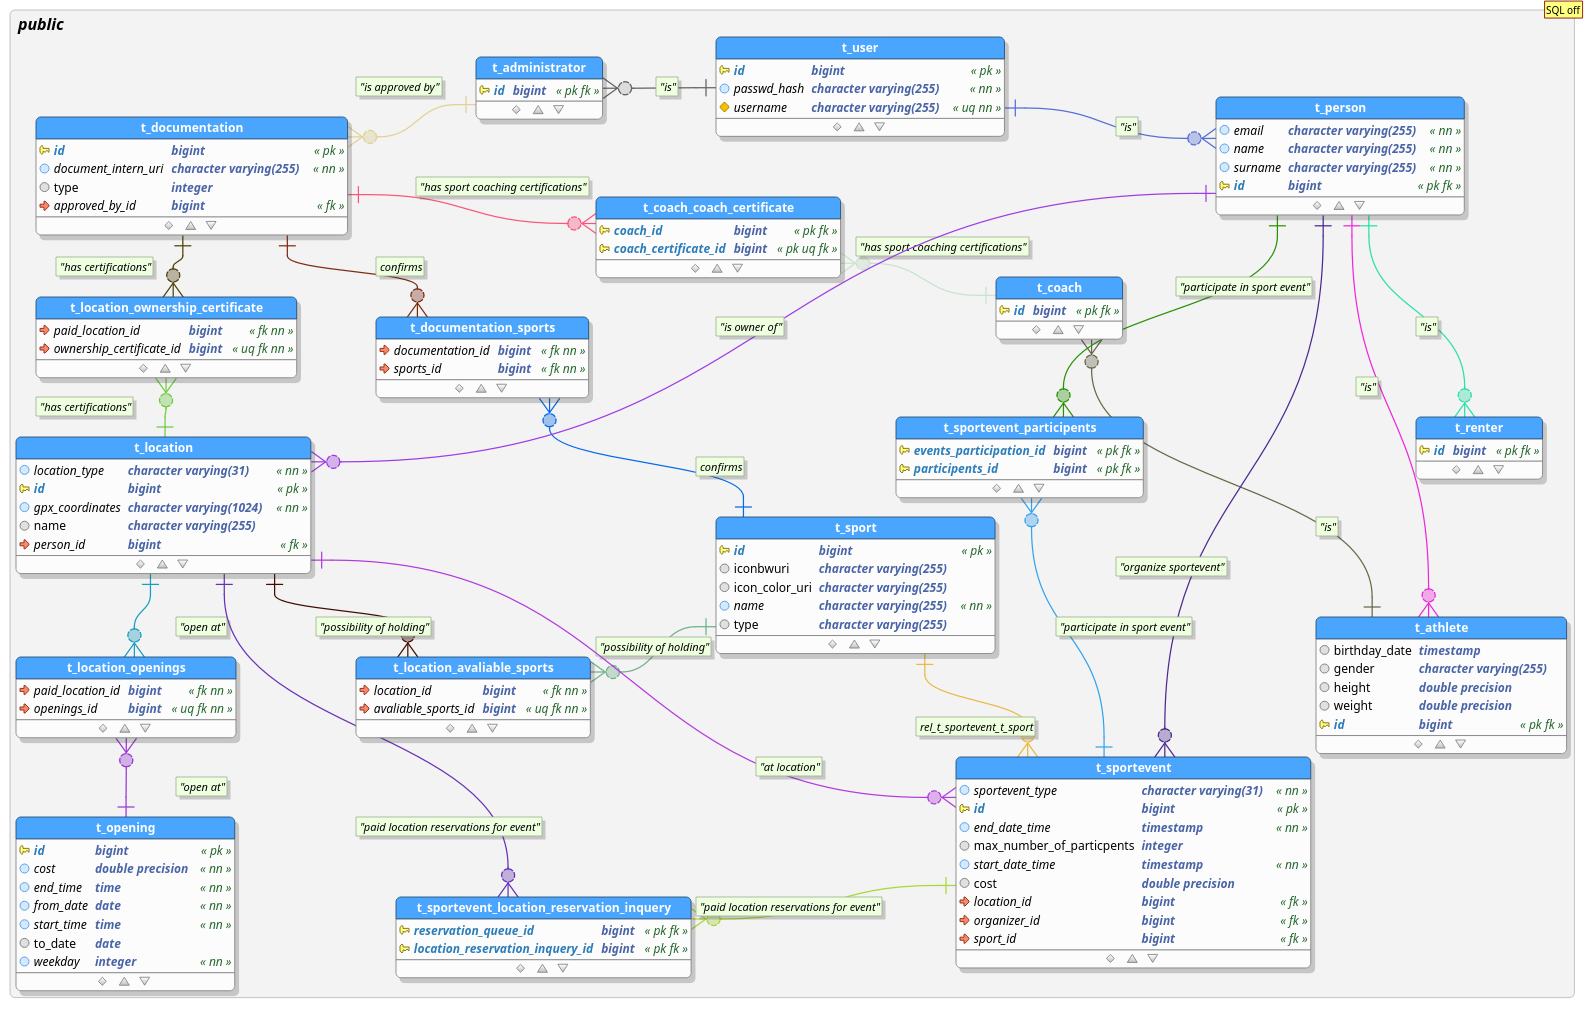
\includegraphics[scale=0.60]{slike/bazapodataka.png}
				\caption{Dijagram baze podataka}
			\end{figure}
			
		\end{landscape}
		\restoregeometry
			
			\eject
		\newgeometry{left=0.5cm,bottom=0.5cm,right=0.5cm,top=0.5cm}
		\begin{landscape}
		
			\section{Dijagram razreda}
			\thispagestyle{empty}
			\begin{figure}[ht!]
				\centering
				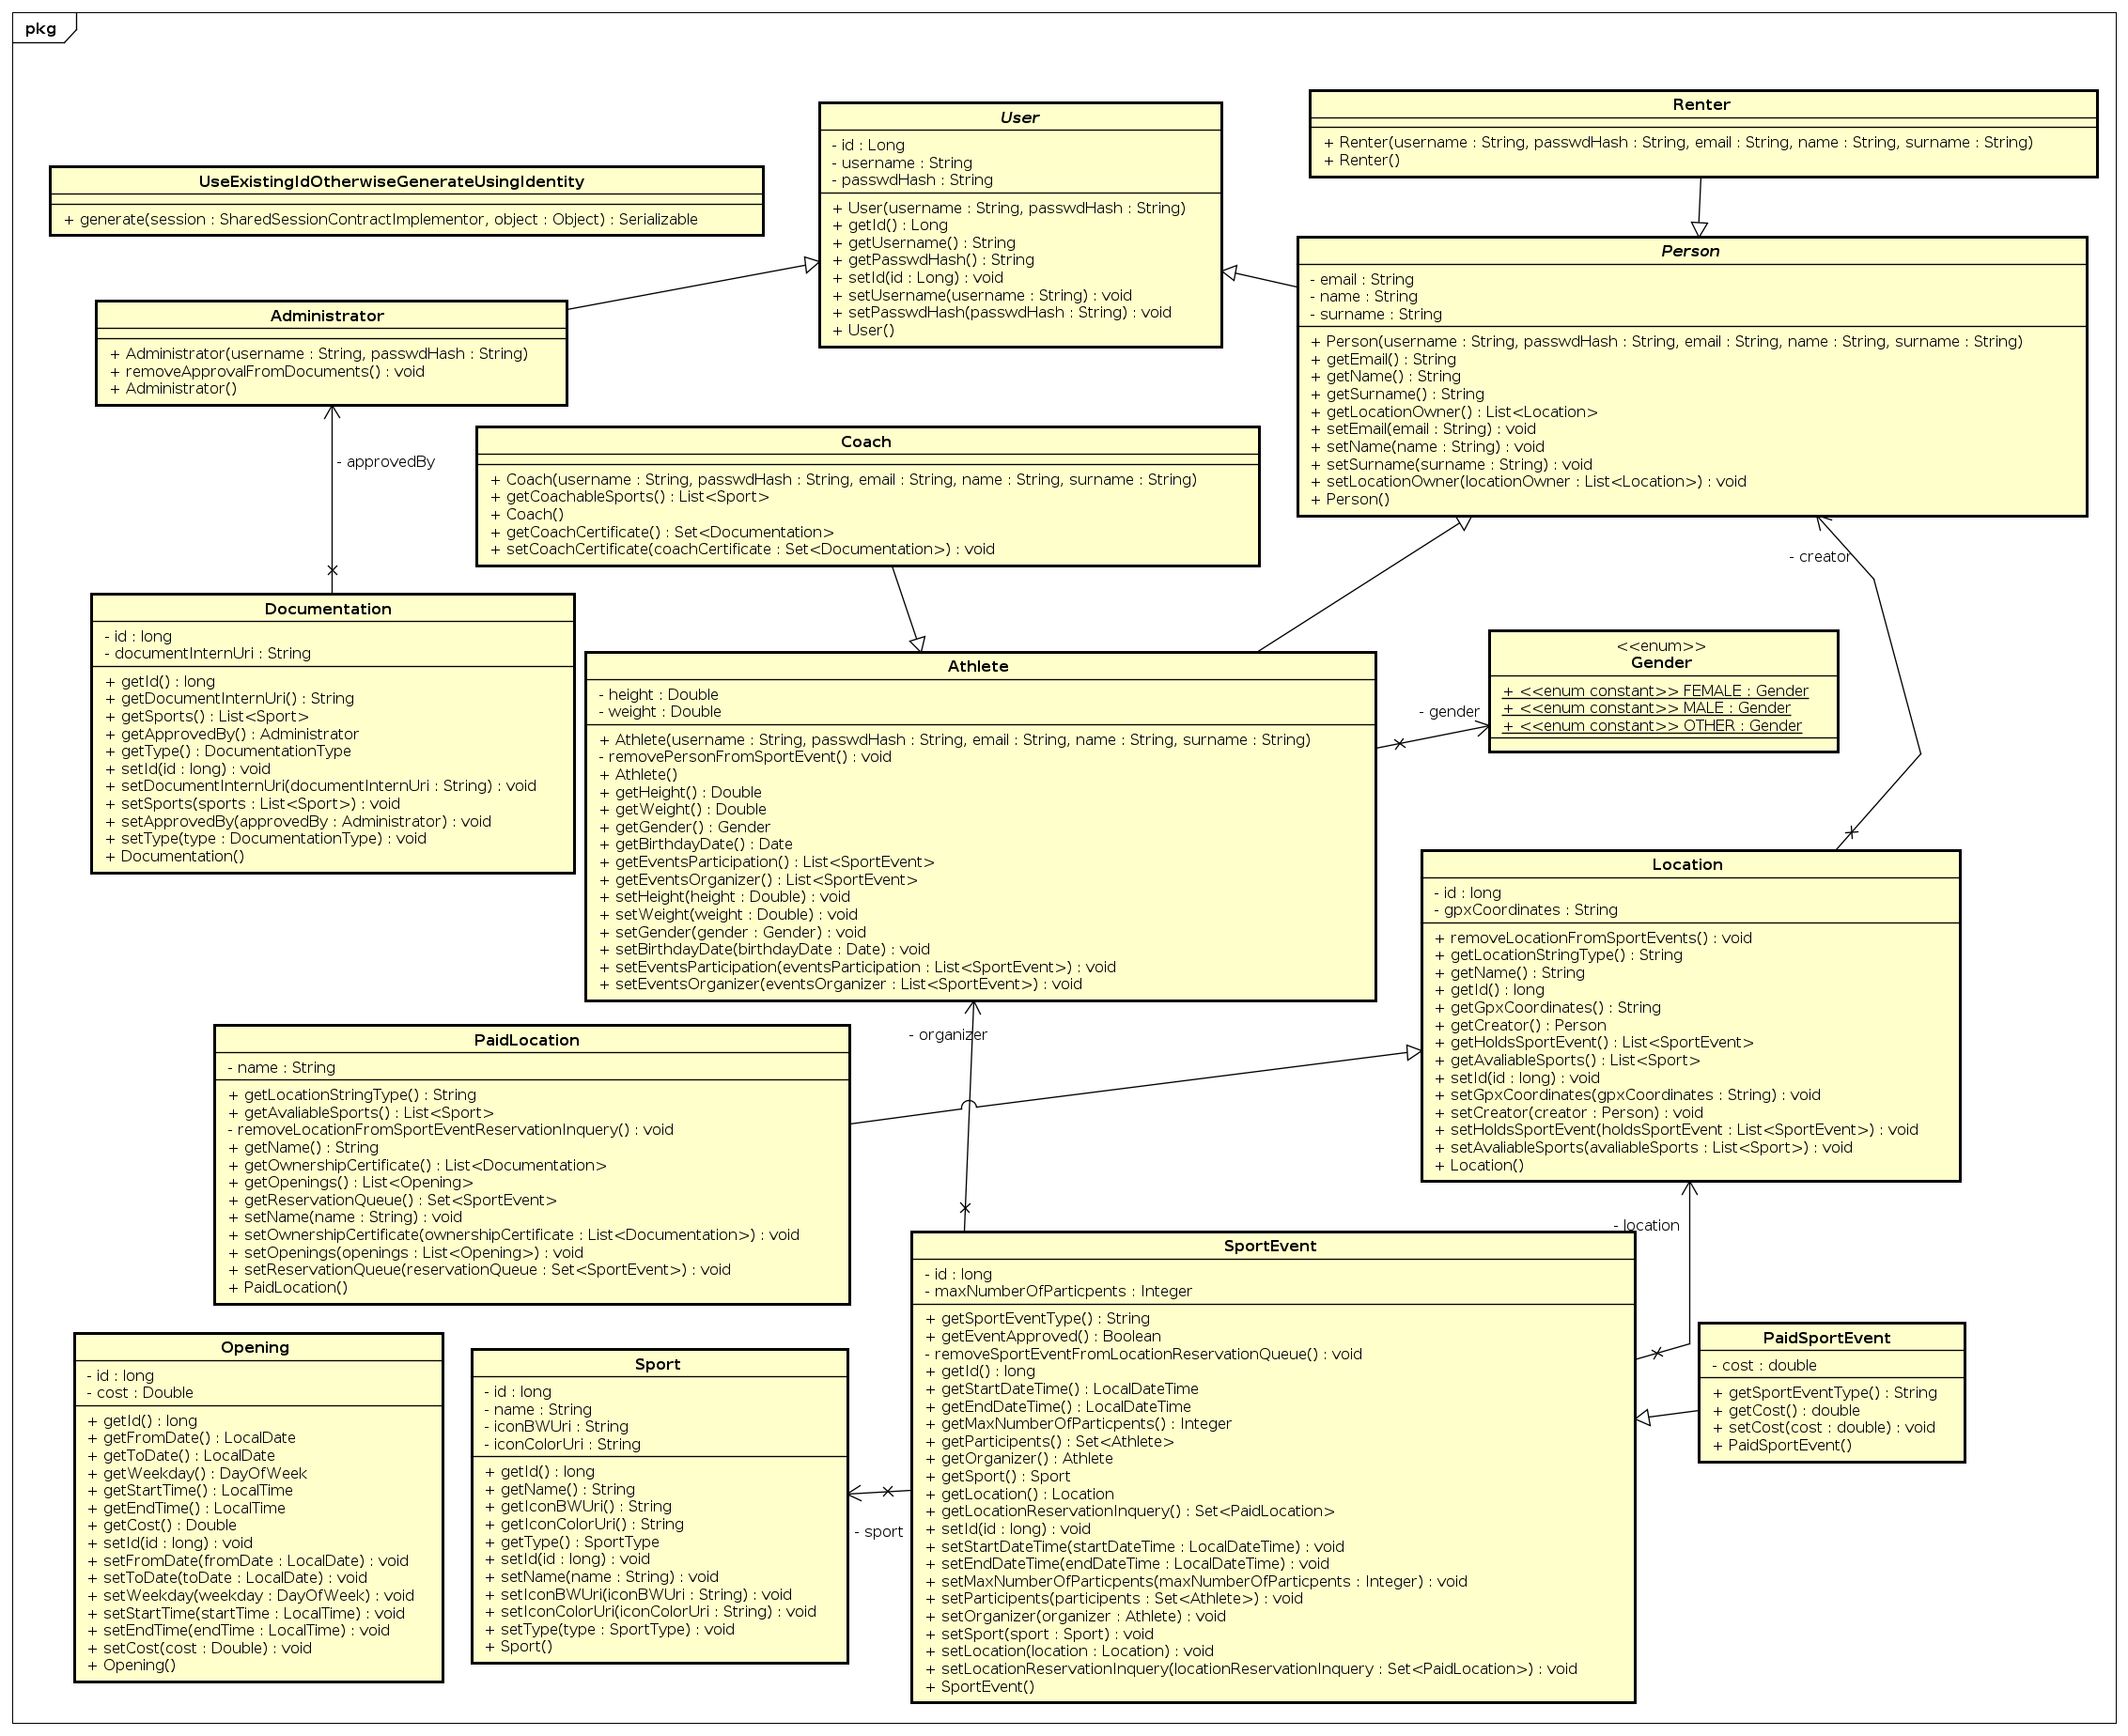
\includegraphics[scale=0.35]{dijagrami/dijagram_razreda_domena.png}
				\caption{Dijagram razreda}
			\end{figure}
			
		\end{landscape}
		\restoregeometry
		\eject
		
		Razred \textbf{User} predstavlja registriranog korisnika koji sadrži atribute username i password. Različite vrste korisnika reprezentiramo razredima Administrator, Person, Athlete, Coach, Renter.\\
		Razred \textbf{Person} nasljeđuje User i predstavlja fizičku osobu te sadrži osobne podatke. \textbf{Athlete} nasljeđuje razred Person i predstavlja sportaša, dok \textbf{Coach} nasljeđuje razred Athlete.\\
		Razred \textbf{Coach} sadrži i referencu na svoju dokumentaciju koja potvrđuje da je službeni trener za određene sportove.\\
		Razred \textbf{Renter} predstavlja iznajmljivača i nasljeđuje razred Person. Razred \textbf{Administrator} nasljeđuje razred User te sadrži referencu na sve dokumente (\textbf{Documentation}) koje je potvrdio.\\
		Razred \textbf{Location} predstavlja lokaciju nekog sportskog okupljanja kojeg je kreirao sportaš, te sadrži atribut GPXCoordinates u kojem su zapisane GPX koordinate objekta. Lokacija sadrži referencu na osobu (Person) koja ju je napravila.\\
		Razred \textbf{PaidLocation} predstavlja lokaciju koju je iznajmljuje iznajmljivač (\textbf{Renter}). Plaćena lokacija sadrži popis radnih sati (\textbf{Opening}) i popis sportova (\textbf{Sport}) koji se mogu igrati na navedenoj lokaciji. Također lokacija koja se iznajmljuje mora imati dokumentaciju o objektu (\textbf{Documentation}) koju potvrđuje Administrator.\\
		Razred \textbf{Opening} predstavlja jedan segment radnog vremena. Segment je definiran danom u tjednu (\textbf{weekday}) i početnim (\textbf{start\_time}) i završnim satom (\textbf{end\_time}). Takav segment se ponavlja sve dok je unutar područja aktivnosti definiranog s početnim datumom (\textbf{from\_date}) i završnim datumom (\textbf{to\_date}).\\
		Razred \textbf{SportEvent} predstavlja događaj koje ovisno o tipu može biti sportsko okupljanje ili profesionalni trening. SportEvent sadrži referencu na lokaciju događaja (\textbf{Location}) i na osobu koja je napravila događaj (\text{Athlete}). Ako događaj iznajmljuje objekt (\textbf{PaidLocation}) tada iznajmljivač putem atributa location\_approved potvrđuje rezervaciju objekta.\\
		Razred \textbf{Documentation} predstavlja dokumentaciju te sadrži interni url PDF datoteke koja je prenesena. Također sadrži i referencu na sportove koji se odnose na dokumentaciju. Dokumentaciju potvrđuje administrator. Razred \textbf{Sport} sadrži informacije vezane uz jedan sport. 
		\eject
		
		\newgeometry{left=2.0cm,bottom=0.5cm,right=0.5cm,top=0.5cm}
		\begin{landscape}
			\thispagestyle{empty}

			\begin{figure}[ht!]
				\centering
				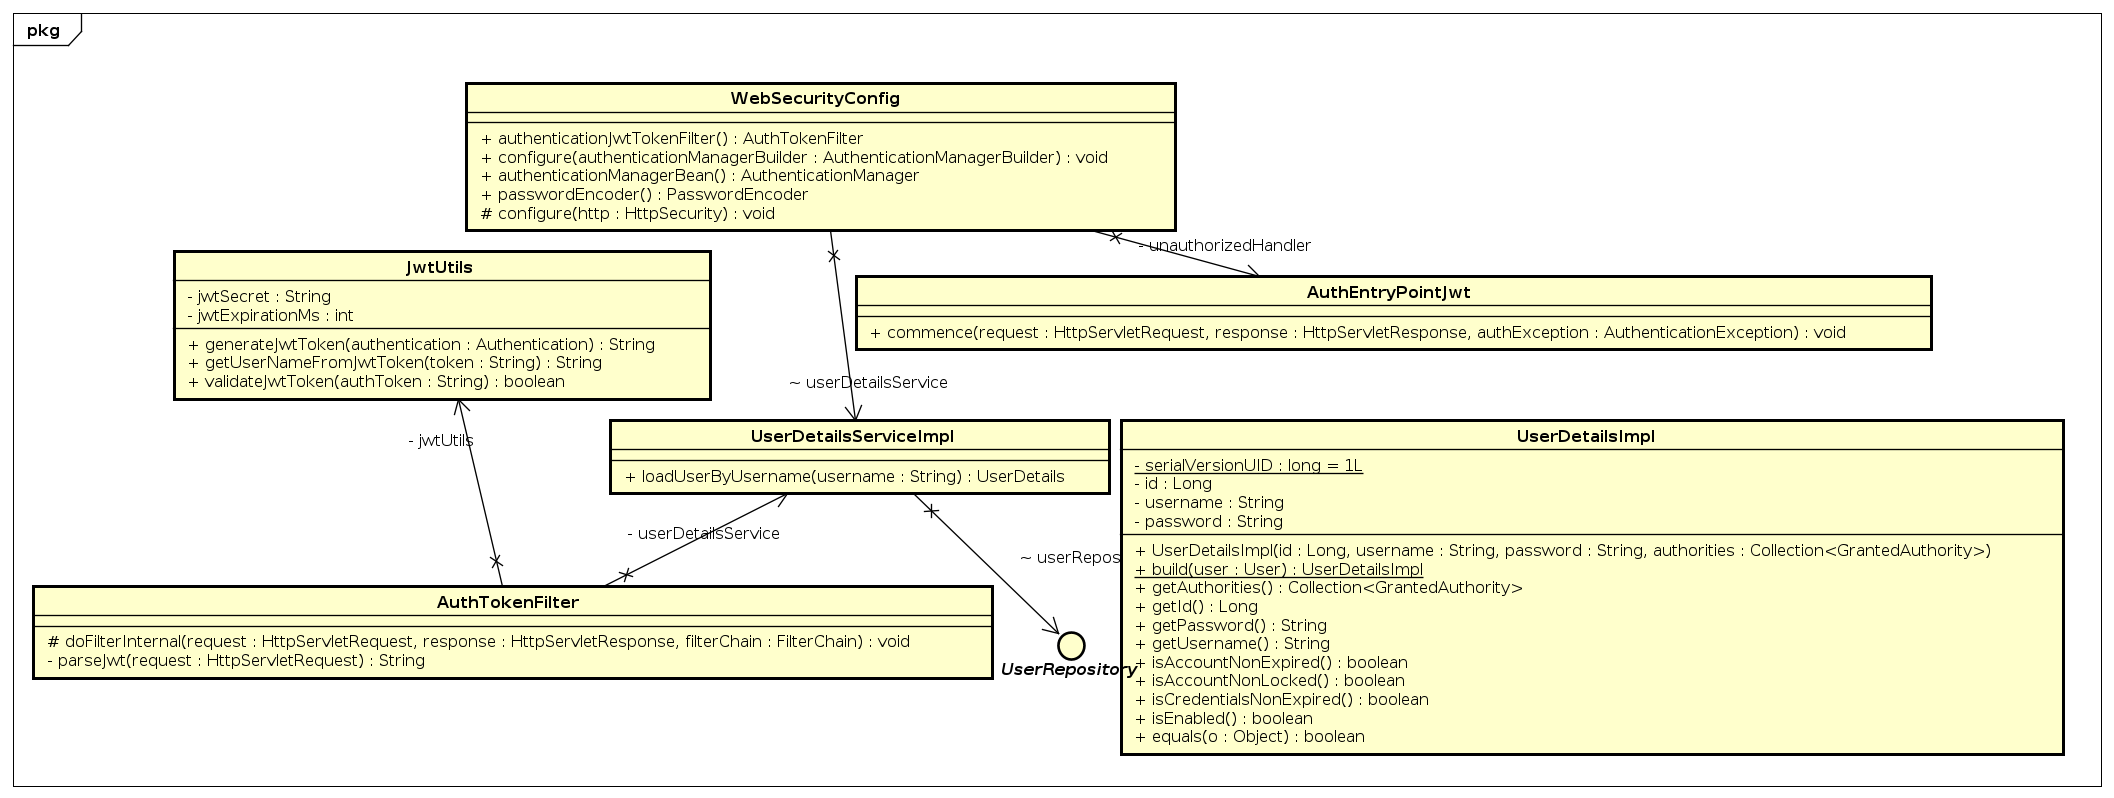
\includegraphics[scale=0.50]{dijagrami/dijagram_razreda_JWT_security.png}
				\caption{Dijagram razreda JWT autentifikacije}
			\end{figure}
			
		\end{landscape}
		\restoregeometry
		\eject
		
		U razredu \textbf{WebSecurityConfig} koji implementira WebSecurityConfigurerAdapter sučelje postavljamo opcije vezane uz Spring Security. Razred \textbf{AuthEntryPointJwt} implementira AuthenticationEntryPoint te se metoda commence pokreće svaki put kada neregistrirani korisnik pristupi zaštićenom sadržaju, te se vraća HTTP 401 UNAUTHORIZED. Kako bi Spring Security omogućili da učita korisnika implementiramo sučelje UserDetailsService u razredu \textbf{UserDetailsServiceImpl}, a podatke samog korisnika spremamo u razredu \textbf{UserDetailsImpl}. Razred \textbf{JwtUtils} pruža metode za parsiranje, generiranje, i validaciju JWT.
		
		\begin{figure}[H]
			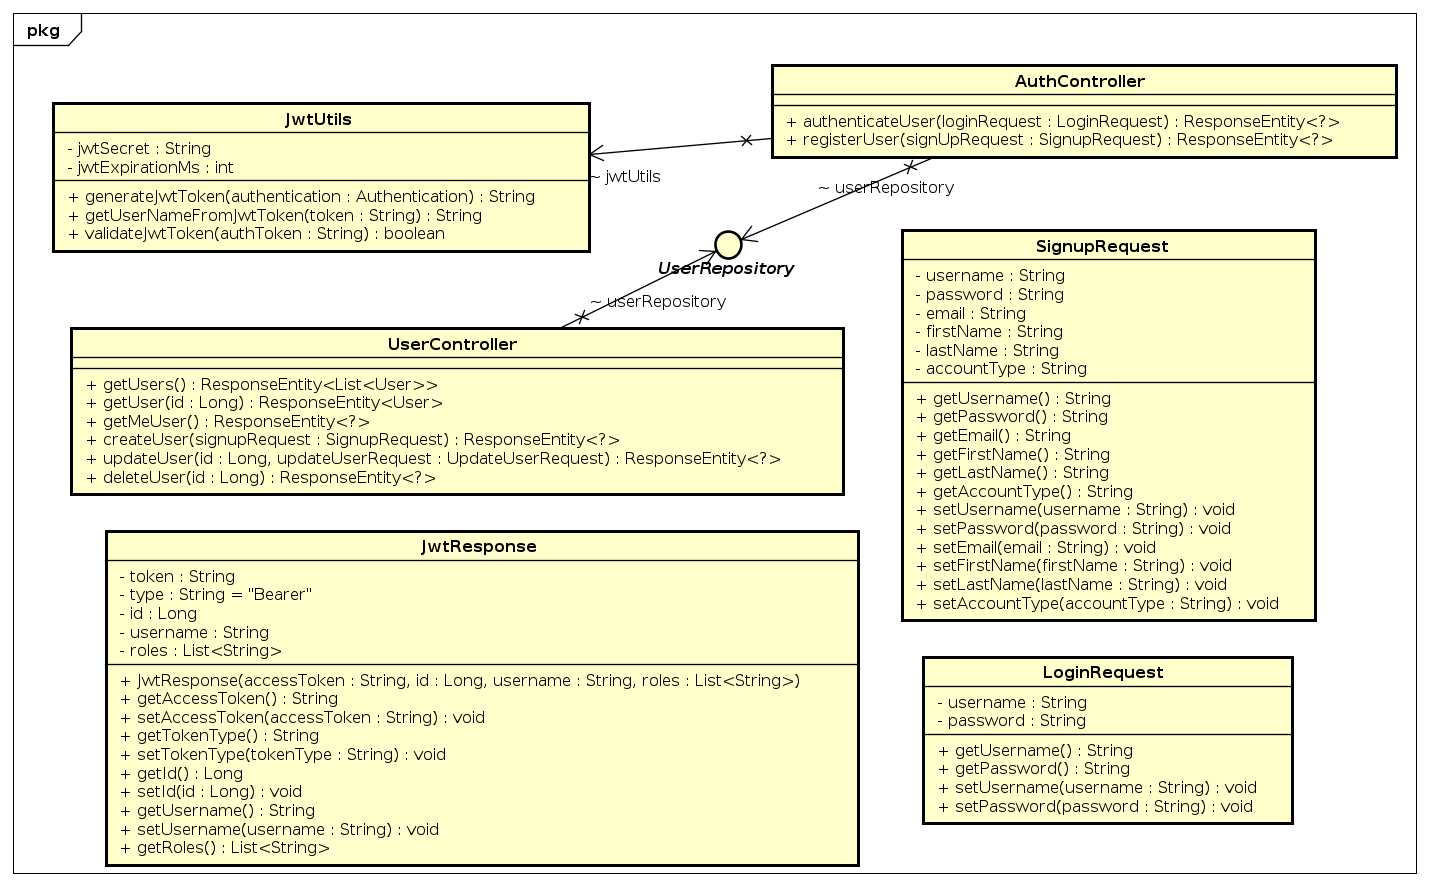
\includegraphics[width=\textwidth]{dijagrami/dijagram_razreda_login.png}
			\caption{Dijagram razreda prijave u sustav}
		\end{figure}
	
		Razred \textbf{AuthController} poslužuje zahtjeve za prijavu i registraciju koje prima pomoću razreda \textbf{LoginRequest} i \textbf{SignupRequest}. Dok razred \textbf{ProfileController} poslužuje osnovne informacije o prijavljenom korisniku.
		
		
		\begin{figure}[H]
			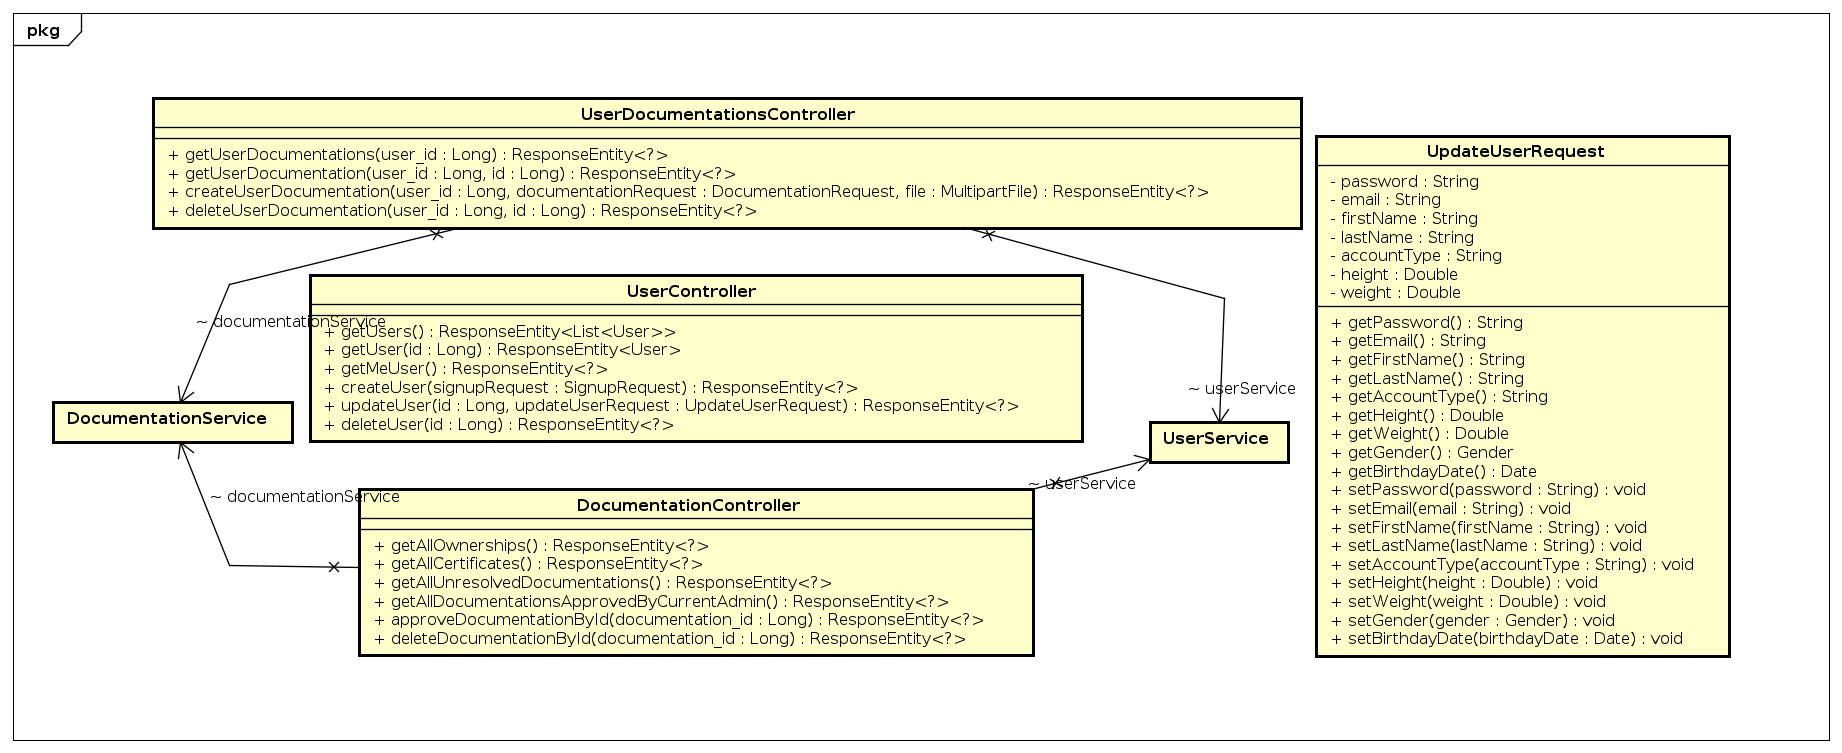
\includegraphics[width=\textwidth]{dijagrami/dijagram_razreda_user.png}
			\caption{Dijagram razreda osnovnih korisničkih funkcionalnosti}
		\end{figure}
		Razred \textbf{UserController} omogućuje pregled osnovnih informacija o korisniku. Također pomoću podataka koje prima preko razreda \textbf{UpdateUserRequest} može vršiti osvježavanje podataka korisnika. Razred \textbf{UserDocumentationController} poslužuje zahtjeve za predaju dokumentacija trenera. Razred \textbf{DocumentationController} služi za pregled dokumentacija trenera i lokacija od strane administratora te povrđivanje ili uklanjanje. 
		
	
	
		\begin{figure}[H]
			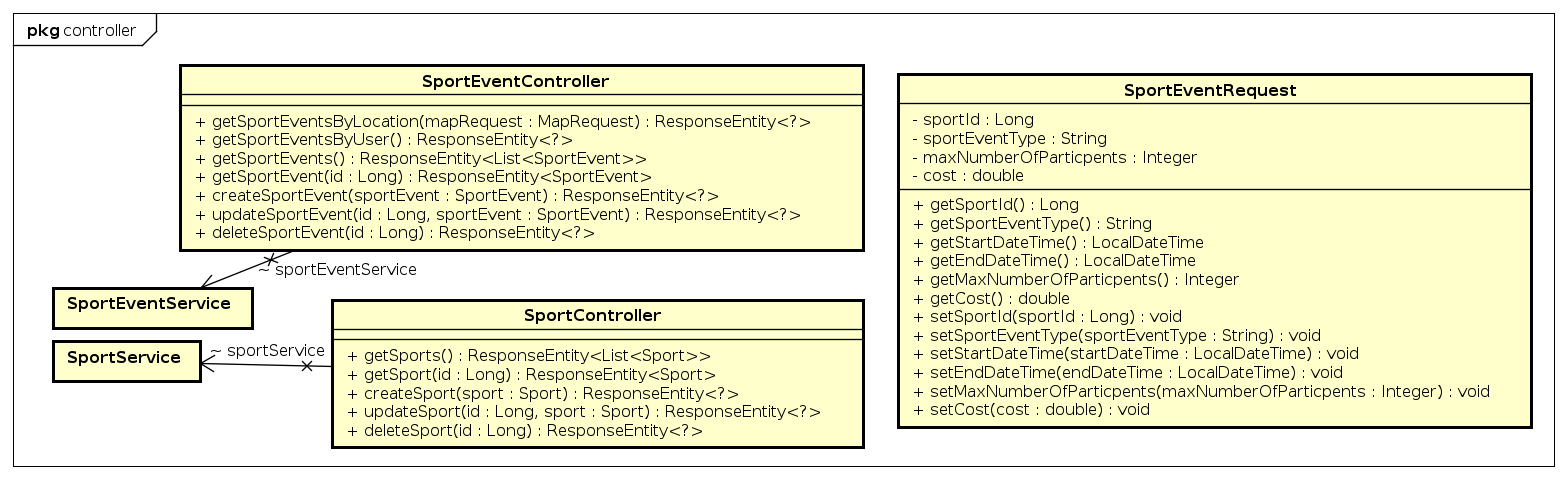
\includegraphics[width=\textwidth]{dijagrami/dijagram_razreda_sportevente.png}
			\caption{Dijagram razreda funkcionalnosti sportskih okupljanja}
		\end{figure}
	
		Razred \textbf{SportEventController} poslužuje osnovne informacije o sportskim okupljanjima. Također omogućuje dobivanje podataka o sportskim okupljanjima na nekoj lokaciji. Razred \textbf{SportController} služi za dohvaćanje podataka o sportovima koji su dostupni unutar aplikacije.
	
	
		\newgeometry{left=2.0cm,bottom=0.5cm,right=0.5cm,top=0.5cm}
		\begin{landscape}
			\thispagestyle{empty}
			
			\begin{figure}[ht!]
				\centering
				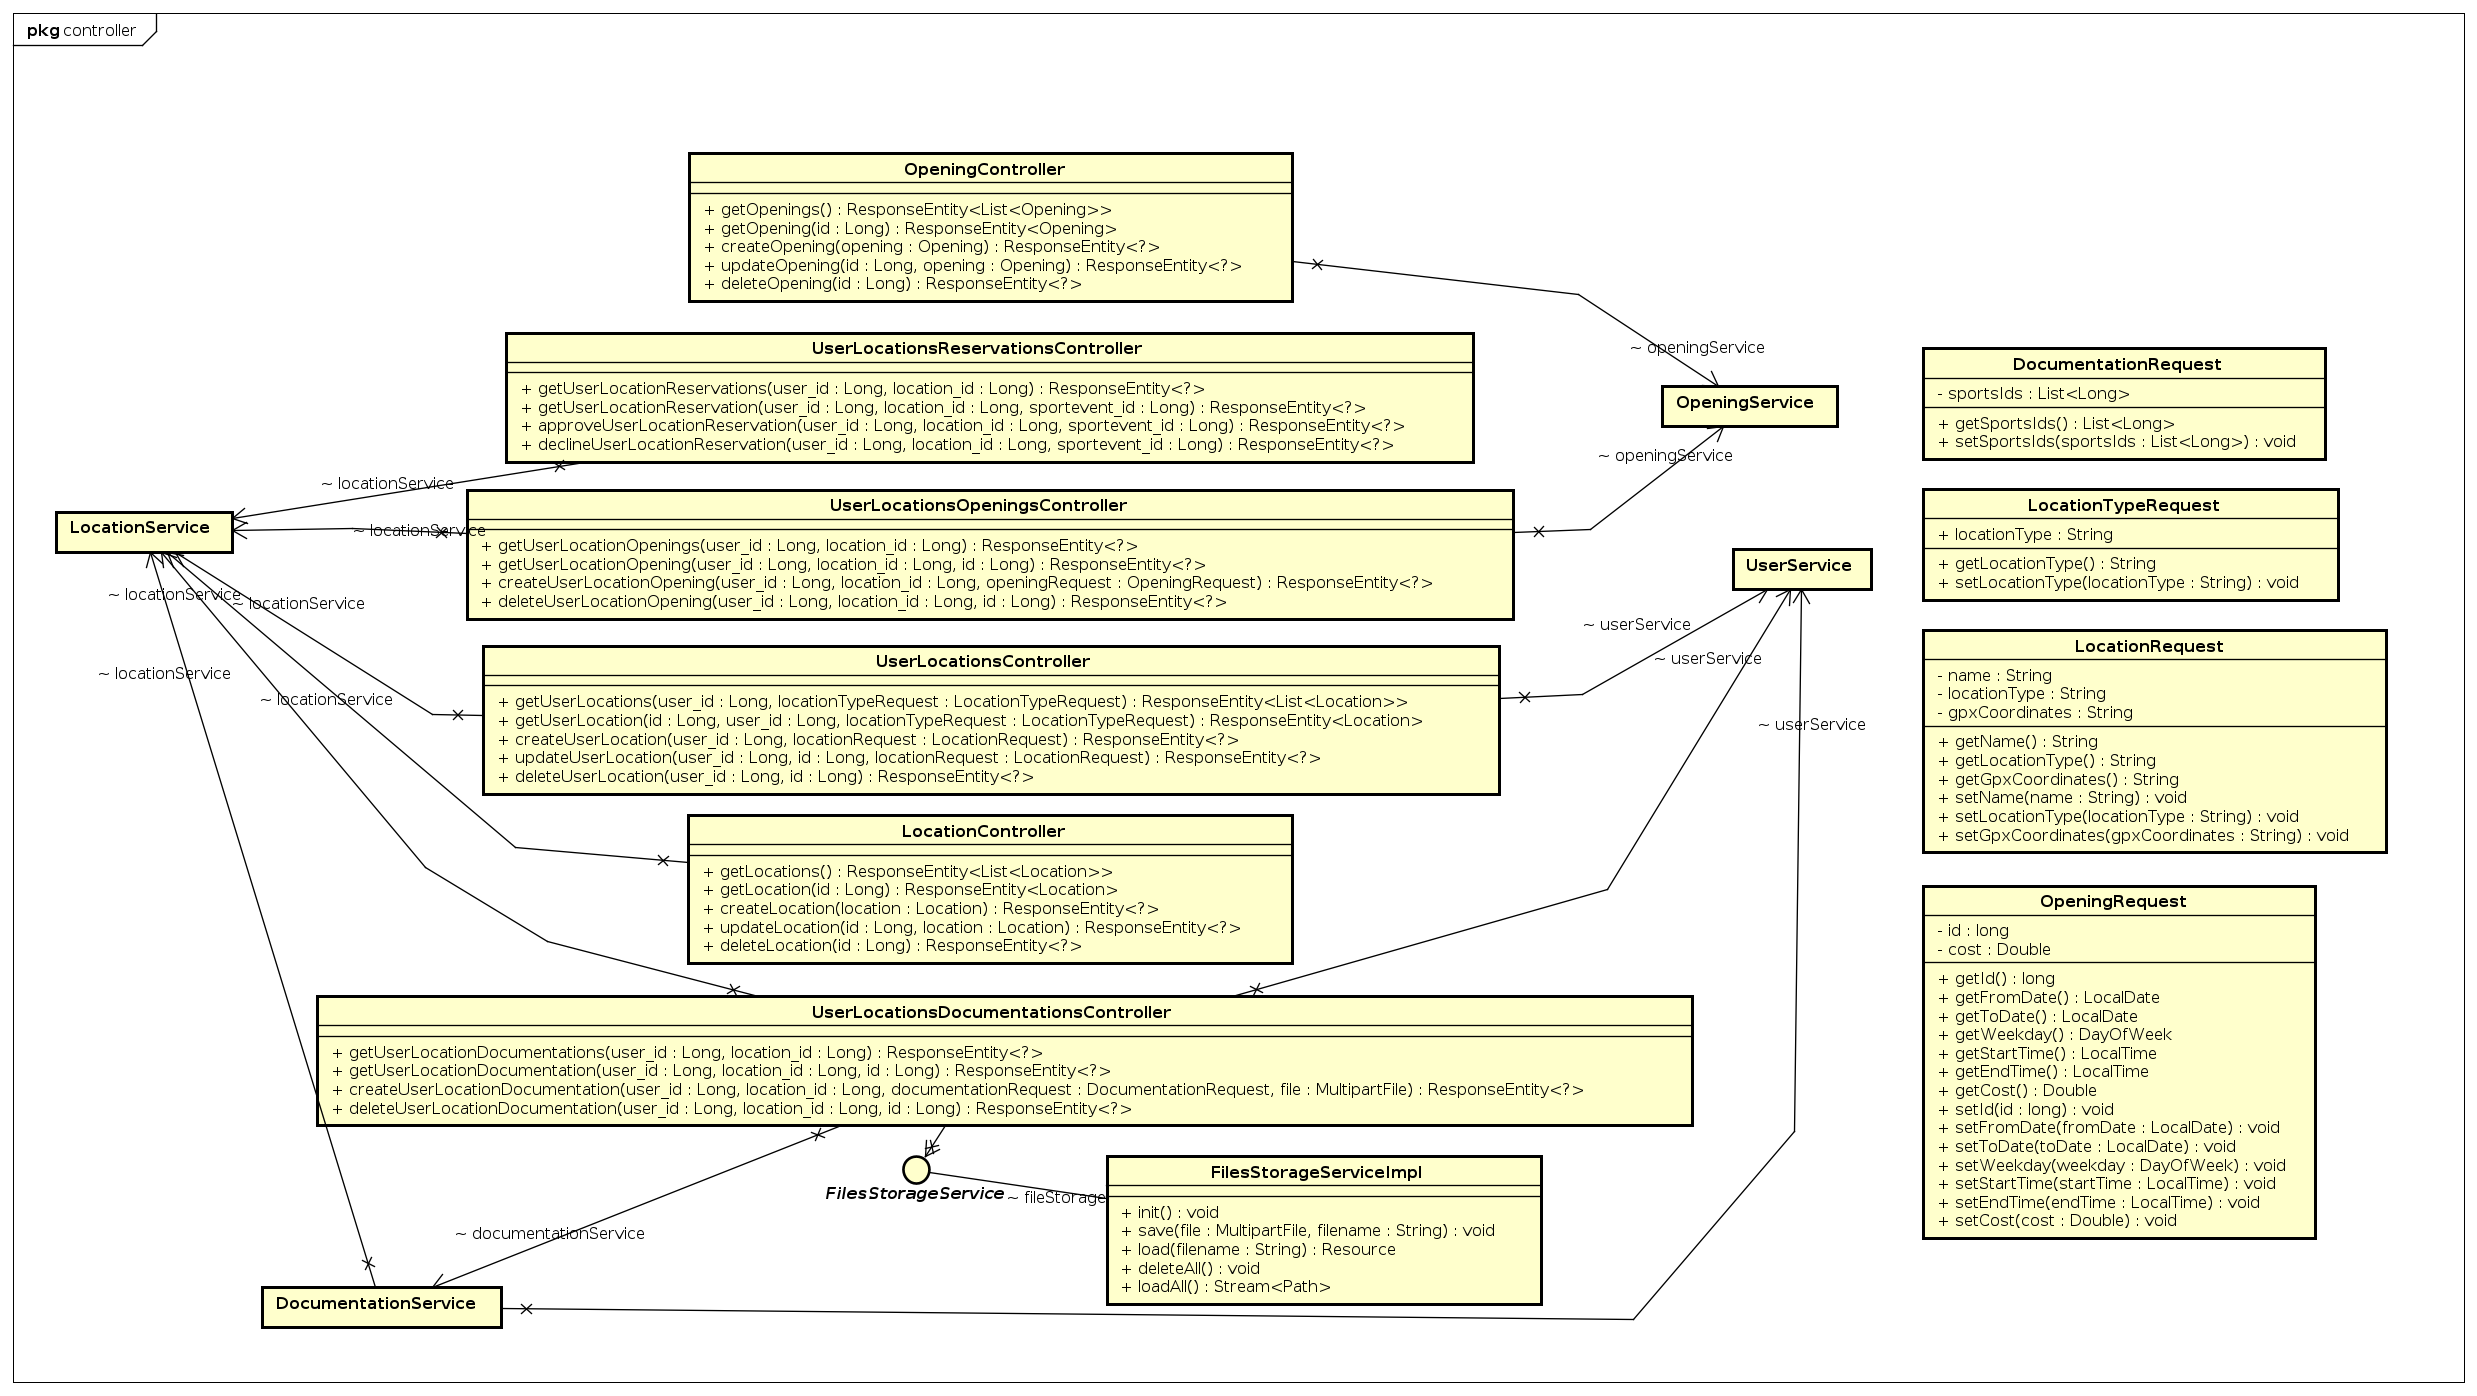
\includegraphics[scale=0.40]{dijagrami/dijagram_razreda_za_lokacije.png}
				\caption{Dijagram razreda funkcionalnost lokacija}
			\end{figure}
			
		\end{landscape}
		\restoregeometry
		\eject
	
		\newgeometry{left=2.0cm,bottom=0.5cm,right=0.5cm,top=0.5cm}
		\begin{landscape}
			\thispagestyle{empty}
			
			\begin{figure}[ht!]
				\centering
				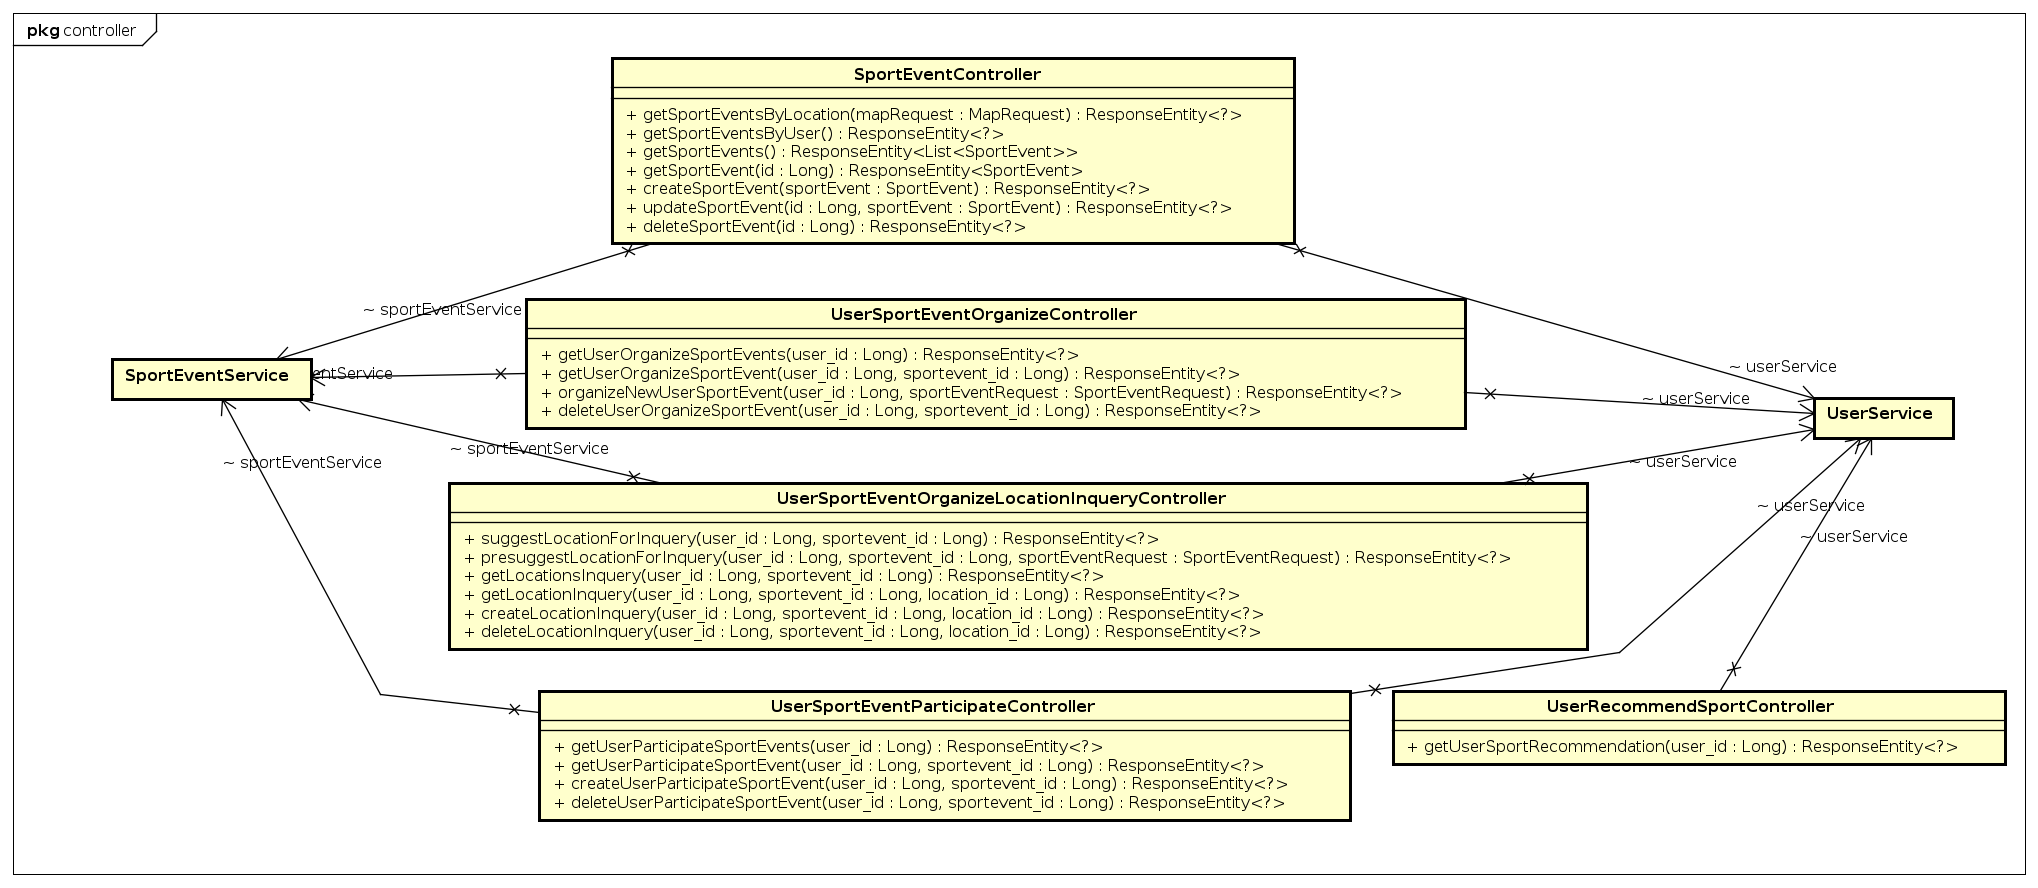
\includegraphics[scale=0.50]{dijagrami/dijagram_razreda_sportevent_lokacije.png}
				\caption{Dijagram razreda veze lokacija i sportskih okupljanja}
			\end{figure}
			
		\end{landscape}
		\restoregeometry
		\eject
	
		Razred \textbf{OpeningController} poslužuje informacije o radnom vremenu lokacije. Razred \textbf{LocationController} omogućuje pregled lokacija. Razred \textbf{UserLocationController} služi za upravljanje korisnikovih lokacija. \textbf{UserLocationsOpenings} omogućuje postavljanje radnog vremena korisnikovoj lokaciji koja se plaća. Razred \textbf{UserLocationsReservationsController} omogućuje potvrđivanje rezervacije nekog sportskog okupljanja na pojedinoj lokaciji. Razred \textbf{UserLocationsDocumentationsController} omogućuje iznajmljivačima prijenos dokumentacija na poslužitelj.
		\hfill\break
		
		Razred \textbf{UserSportEventOrganizeController} omogućuje sportašu slanje zahtjeva za organiziranje sportskih okupljanja. Svako sportsko okupljanje može zatražiti rezervaciju plaćene lokacije preko razreda \textbf{UserSportEventOrganizeLocationInqueryController}. Sportaš preko razreda \textbf{UserSportEventParticipateController} se može prijaviti na sportsko okupljanje.
	
%			\textit{Potrebno je priložiti dijagram razreda s pripadajućim opisom. Zbog preglednosti je moguće dijagram razlomiti na više njih, ali moraju biti grupirani prema sličnim razinama apstrakcije i srodnim funkcionalnostima.}\\
			
%			\textbf{\textit{dio 1. revizije}}\\
			
%			\textit{Prilikom prve predaje projekta, potrebno je priložiti potpuno razrađen dijagram razreda vezan uz \textbf{generičku funkcionalnost} sustava. Ostale funkcionalnosti trebaju biti idejno razrađene u dijagramu sa sljedećim komponentama: nazivi razreda, nazivi metoda i vrste pristupa metodama (npr. javni, zaštićeni), nazivi atributa razreda, veze i odnosi između razreda.}\\
%			
%			\textbf{\textit{dio 2. revizije}}\\			
%			
%			\textit{Prilikom druge predaje projekta dijagram razreda i opisi moraju odgovarati stvarnom stanju implementacije}
			
			
			
			\eject
		
		\section{Dijagram stanja}
			Na slici 4.7 je prikazan dijagram stanja za iznajmljivanje prostora za sport. Korisnik s početne stranice "Naslovnica" klikom na "Iznajmi prostor za sport" dolazi na stranicu za iznajmljivanje prostora za sport. Na toj stranici korisnik može pregledati dostupne prostore za sport, nakon odabira prostora, korisnik odabire dostupan datum i vrijeme termina. Prije klika na "Potvrdi rezervaciju" korisnik može odustati od rezervacije klikom na "Odustani" i vratiti se nazad na stranicu za pregled dostupnih prostora za sport. Nakon odabira prostora, datuma i termina korisnik završava rezervaciju klikom na "Potvrdi rezervaciju" te čeka potvrdu rezervacije. Nakon što sustav potvrdi rezervaciju korisnik bira hoće li napraviti još rezervacija ili ne, ako odabere da želi napraviti još rezervacija sustav ga vrati na stranicu za iznajmljivanje prostora za sport, inače ga vrati na "Naslovnicu". Ako dođe do greške prilikom rezervacije sustav obavijesti korisnika o greški te ga vrati na početnu stranicu za iznajmljivanje. Korisnik se može s početne stranice za iznajmljivanje vratiti na "Naslovnicu" klikom na "Povratak na Naslovnicu".
			
			\begin{figure}[H]
				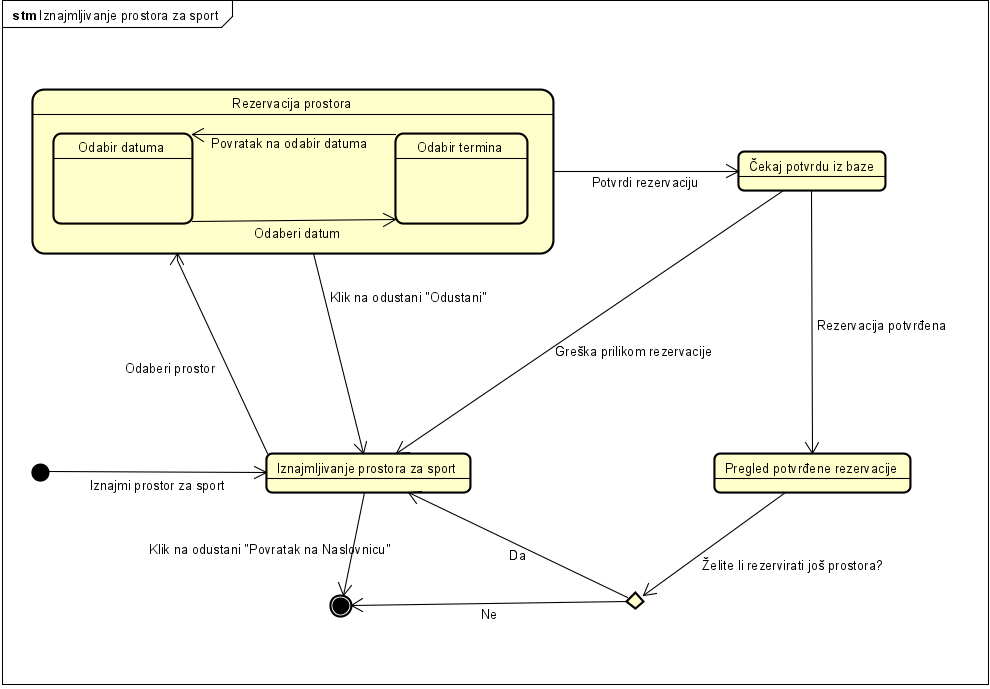
\includegraphics[width=\textwidth]{slike/dijagramStanja.png}
				\caption{Dijagram stanja iznajmljivanja prostora za sport}
			\end{figure}
%			\textbf{\textit{dio 2. revizije}}\\
			
%			\textit{Potrebno je priložiti dijagram stanja i opisati ga. Dovoljan je jedan dijagram stanja koji prikazuje \textbf{značajan dio funkcionalnosti} sustava. Na primjer, stanja korisničkog sučelja i tijek korištenja neke ključne funkcionalnosti jesu značajan dio sustava, a registracija i prijava nisu. }
			
			
			\eject 
		
		\section{Dijagram aktivnosti}
			Na slici 4.8 prikazan je dijagram aktivnosti predaje dokumentacije trenera i prikaz aktivnosti potvrđivanja (ili odbijanja) predane dokumentacije. Trener preda dokumentaciju aplikaciji te aplikacija tu dokumentaciju spremi u bazu. Prilikom spremanja dokumentacije u bazu se zapisuje i podatak da je ta dokumentacija nepotvrđena. Administrator može zatražiti od aplikacije popis svih nepotvrđenih dokumentacija, aplikacija ih uzme iz baze te prikaže administratoru. Administrator pregledava dokumentacije te odlučuje hoće li ih odbaciti (izbrisati) ili potvrditi. Nakon što administrator donese odluku o dokumentaciji trener dobiva obavijest o odluci admnistratora.
			
			\begin{figure}[H]
				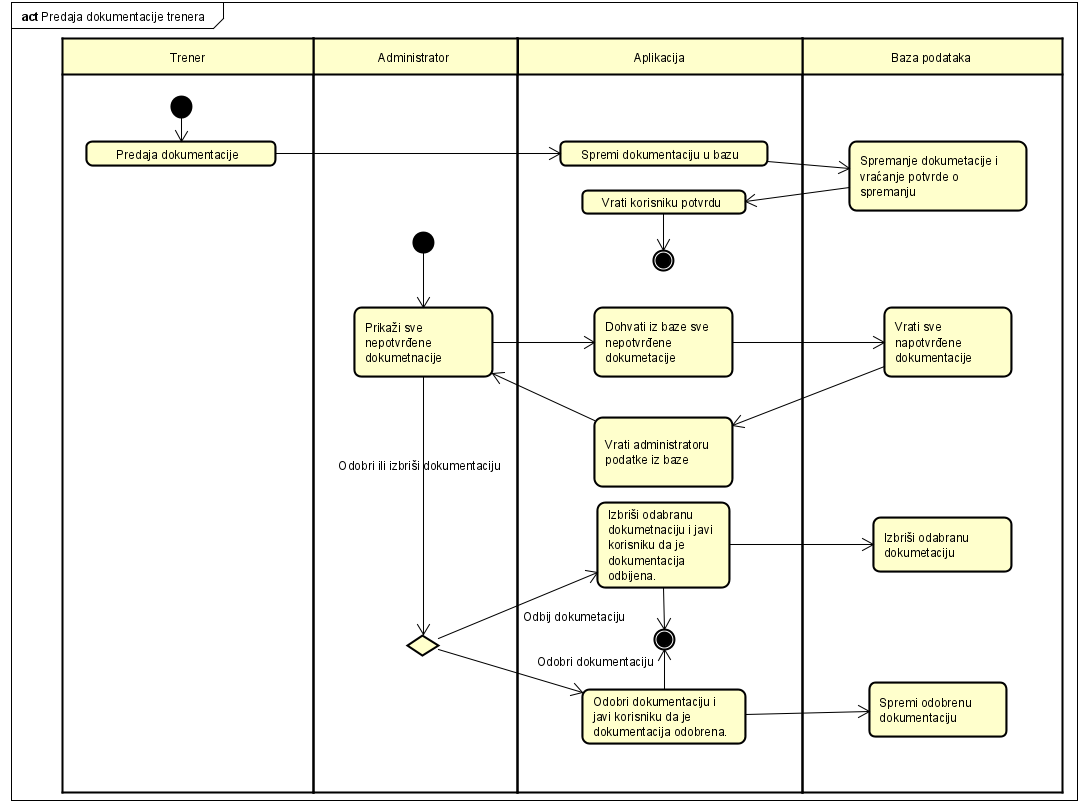
\includegraphics[width=\textwidth]{slike/dijagramAktivnosti.png}
				\caption{Dijagram aktivnosti predaje dokumentacije za trenera}
			\end{figure}
%			\textbf{\textit{dio 2. revizije}}\\
%			
%			 \textit{Potrebno je priložiti dijagram aktivnosti s pripadajućim opisom. Dijagram aktivnosti treba prikazivati značajan dio sustava.}
%			
			\eject
		\section{Dijagram komponenti}
			Dijagram komponenti prikazan na slici opisuje organizaciju i međuovisnost komponenti aplikacije. Aplikaciji se pristupa s web preglednika kojem React biblioteka poslužuje HTML, CSS i Javascript datoteke generirane iz Javascript datoteka predanih biblioteci. React aplikacija odnosno "frontend" dio web aplikacije s "backend" dijelom komunicira slanjem podataka u JSON formatu pomoću programskog paketa Axios. Za osjetljive podatke poput korisničkih informacija podaci se šalju u obliku JWT, odnosno JSON Web Token."Backend" dio web aplikacije s bazom podataka komunicira preko komponente Repository, a podaci dobiveni iz baze podataka koriste se dalje u "backend" dijelu  web aplikacije. "Backend" dio web aplikacije također komunicira s predikcijom sporta strojnim učenjem.
			
			\begin{figure}[H]
				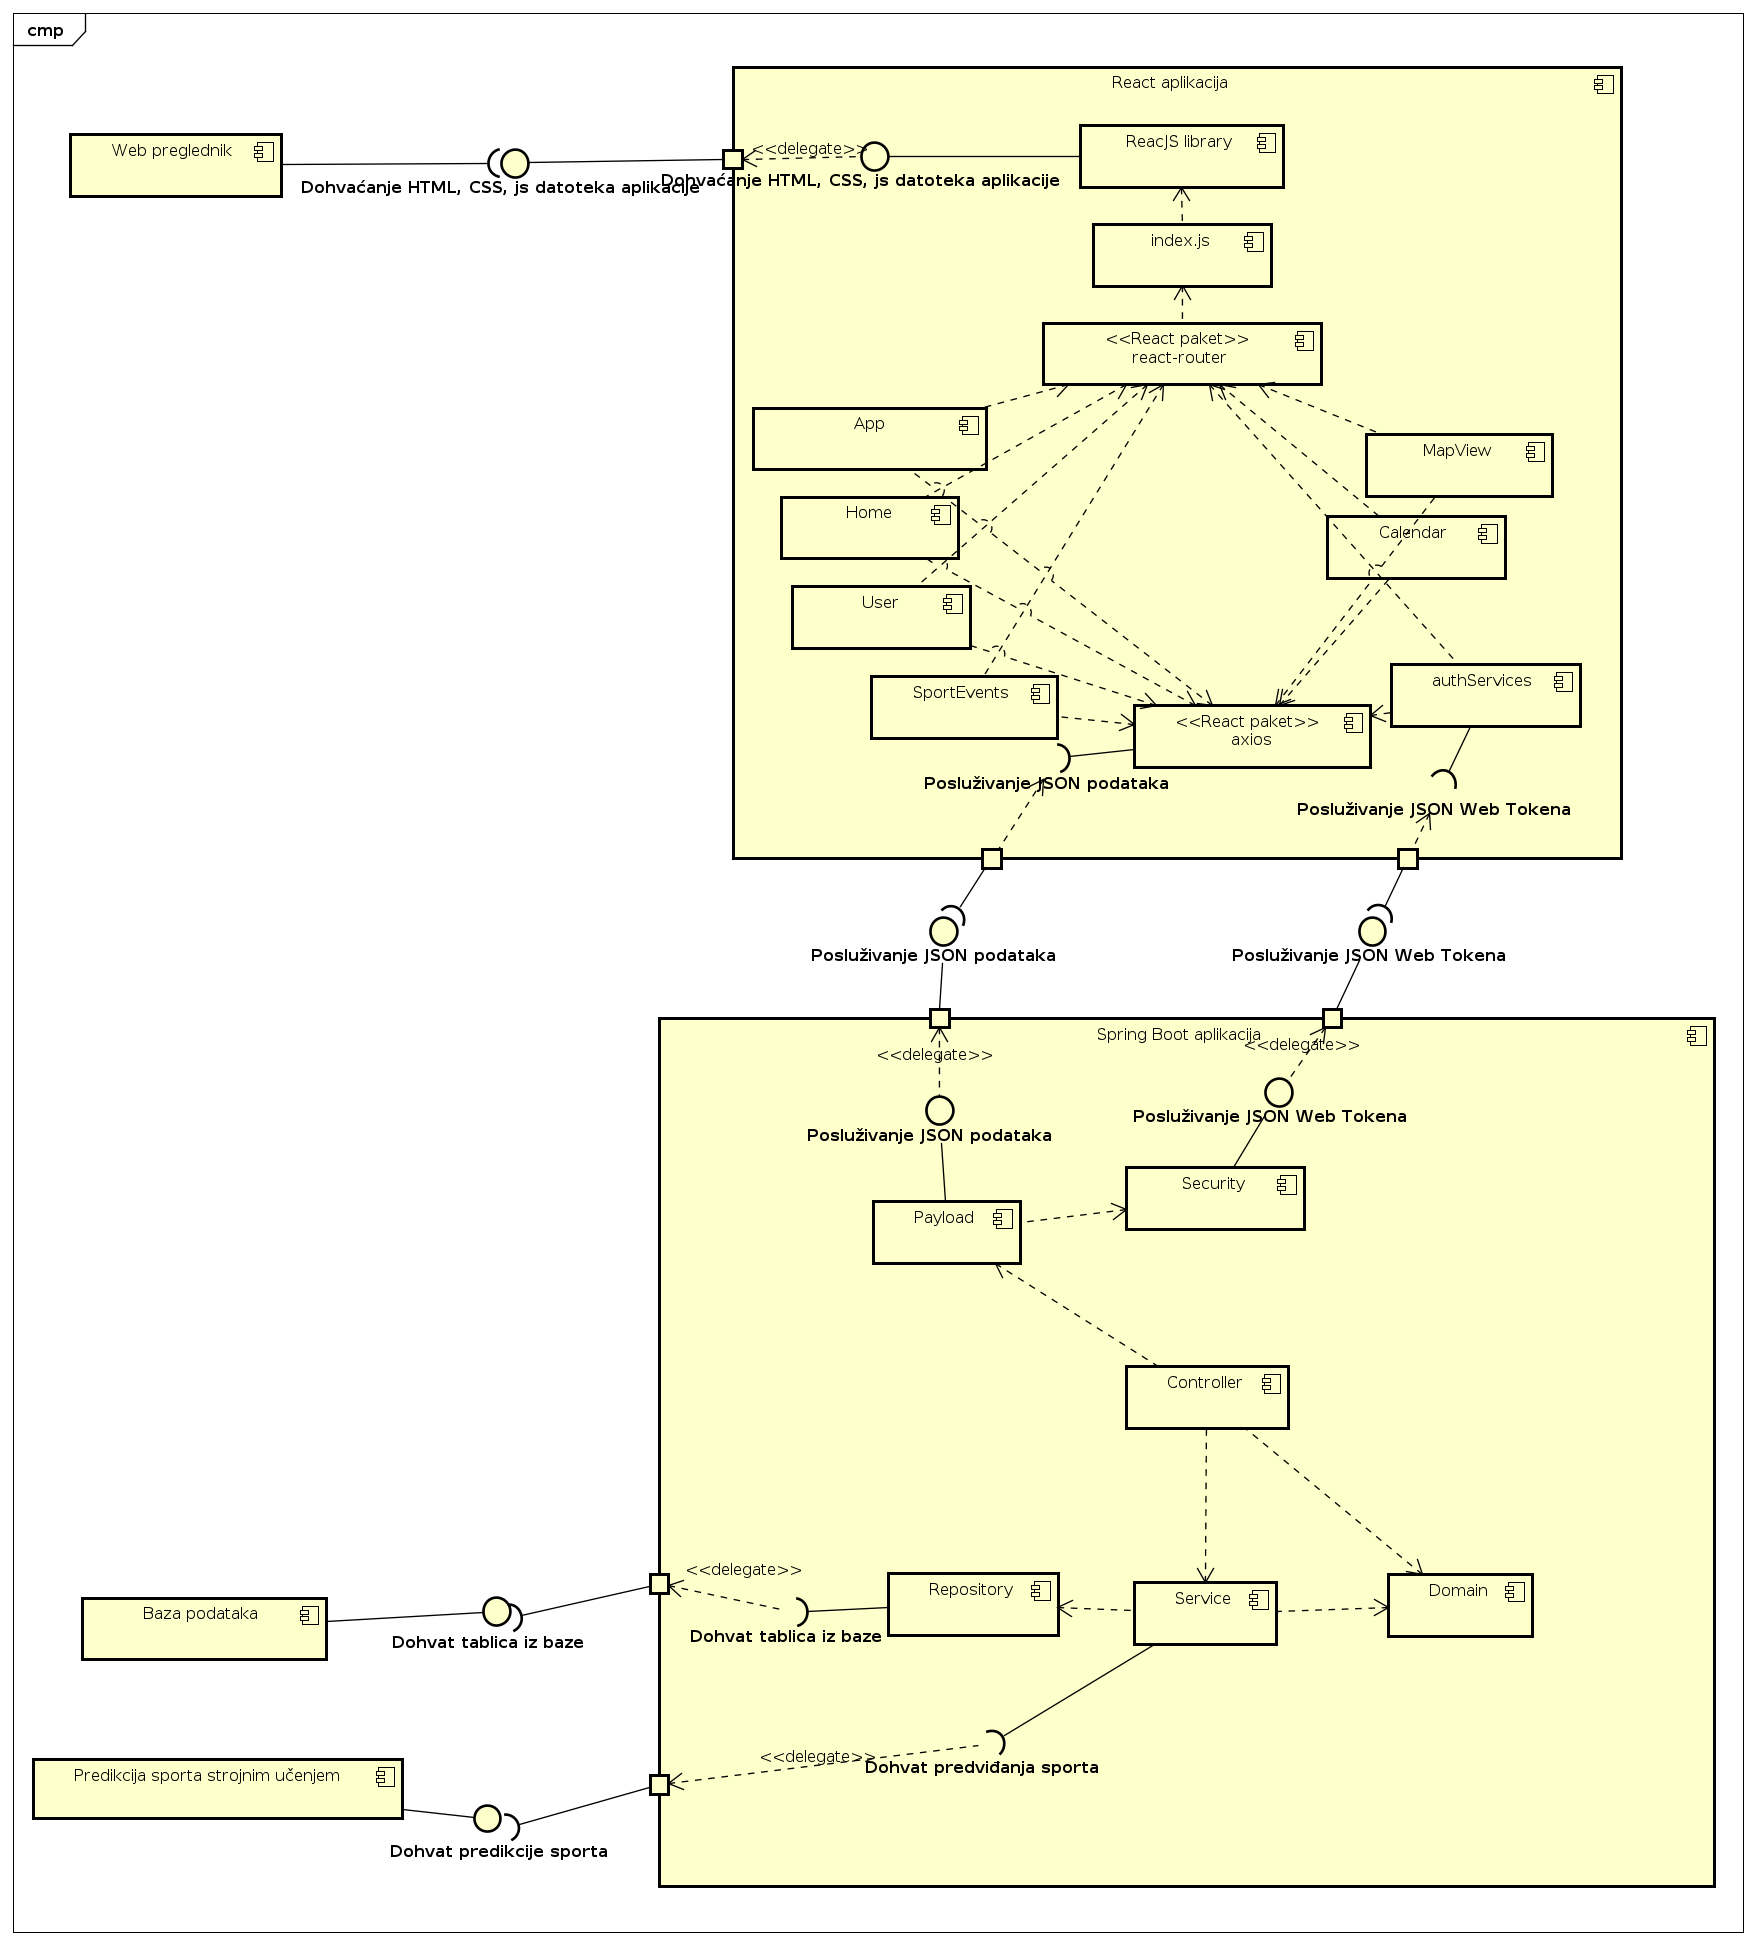
\includegraphics[width=\textwidth]{dijagrami/ComponentDiagram0.png}
				\caption{Dijagram komponenti}
			\end{figure}
		
			\eject
%		
%			\textbf{\textit{dio 2. revizije}}\\
%		
%			 \textit{Potrebno je priložiti dijagram komponenti s pripadajućim opisom. Dijagram komponenti treba prikazivati strukturu cijele aplikacije.}
% Drugi ciklus	
	\chapter{Implementacija i korisničko sučelje}
		
		
		\section{Korištene tehnologije i alati}
		
			\textbf{\textit{dio 2. revizije}}
	
			Komunikacija članova tima realizirana je aplikacijom Discord\footnote{https://discord.com/}. Dokumentacija je pisana u alatu TEXstudio\footnote{https://www.texstudio.org//}, a UML dijagrami crtani su alatom Astah\footnote{https://astah.net/}. Sustav za upravljanje izvornim kodom je Git\footnote{https://git-scm.com/}, a udaljeni repozitorij projekta dostupan je na web platformi GitLab\footnote{https://gitlab.com/}. Kao razvojno okruženje za frontend koristio se Visual Studio Code\footnote{https://code.visualstudio.com/} dok su se  za backend koristili su se IntelliJ IDEA\footnote{https://www.jetbrains.com/idea/} i Eclipse\footnote{https://www.eclipse.org/}. Za izradu aplikacije korištene su tehnologije Spring Boot\footnote{https://spring.io/projects/spring-boot} za backend te React\footnote{https://reactjs.org/} za frontend. Tehnologija Spring Boot zahtjeva programiranje u Javi\footnote{https://www.java.com/en/}, a tehnologija React programiranja u JavaScriptu\footnote{https://www.javascript.com/}. Sustav baze podataka ove aplikacije je PostgreSQL\footnote{https://www.postgresql.org/}. Još treba napisati u čemu smo testirali aplikaciju, uključujući korištene biblioteke.
%			 \textit{
%			 	Detaljno navesti sve tehnologije i alate koji su primijenjeni pri izradi dokumentacije i aplikacije. Ukratko ih opisati, te navesti njihovo značenje i mjesto primjene. Za svaki navedeni alat i tehnologiju je potrebno \textbf{navesti internet poveznicu} gdje se mogu preuzeti ili više saznati o njima}.
			
			
			\eject 
		
	
		\section{Ispitivanje programskog rješenja}
			
			\begin{comment}
			\textbf{\textit{dio 2. revizije}}\\
			 \textit{U ovom poglavlju je potrebno opisati provedbu ispitivanja implementiranih funkcionalnosti na razini komponenti i na razini cijelog sustava s prikazom odabranih ispitnih slučajeva. Studenti trebaju ispitati temeljnu funkcionalnost i rubne uvjete.}
			\end{comment}
			
			\subsection{Ispitivanje komponenti}
			Kako bi se uvjerili u ispravnost pojedinih klasa i metoda proveli smo ispitivanje jedinica (engl. unit testing) nad razredima koji implementiraju temeljne funkcionalnosti. Testove smo napisali tako da ispituju redovne slučajeve, ali i rubne slučajeve.
			Koristili smo javin open source framework za testiranje JUnit.\\
			
			\noindent\textbf{Ispitni slučaj 1: traženje korisnika po korisničkom imenu}\\
			Sljedeća dva testa provjeravaju funkcionalnosti klase userService.
			Klasa userService pruža metodu za dohvat korisnika na temelju njegovog korisničkog imena.
			Tu metodu smo testirali sa validnim korisničkim imenom "athlete" u metodi testFindGoodUsername te sa imenom nepostojećeg korisnika u metodi
			 testFindBadUsername.
			 
			 \begin{lstlisting}[language=Java,caption={findByUsername},label=DescriptiveLabel]
@Test
void testFindGoodUsername() {
  Optional < User > user = userService.findByUsername("athlete");
  assertThat(user.isPresent());
}

@Test
void testFindBadUsername() {
  Optional < User > user = userService.findByUsername("wrongUsername");
  assertThat(user.isEmpty());
}
			 \end{lstlisting}
		
			\noindent Rezultat izvođenja ispitnog slučaja: Ispit je uspješan.

				%tu dodat slike kad se runna JUnit test.
			
			
			\hfill\break
			\noindent\textbf{Ispitni slučaj 2: Dodavanje i spremanje korisnika.}\\
			Slijedećim testom provjerili smo funkcionalnosti stvaranja i dodavanja novog korisnika sportaša. Testirane metode također su dio klase userService.
			
			\begin{lstlisting}[language=Java,caption={testSaveAndFindUser},label=DescriptiveLabel]
@Test
void testSaveAndFindUser() {
  User user = new Athlete("newUsername", "newPassword", "e@mail.com", "name", "surname");
  userService.save(user);
  Optional < User > user1 = userService.findByUsername("newUsername");
  assertThat(user1.isPresent());
}

			\end{lstlisting}
			\noindent Izvođenje ispitanog slučaja: Ispit je uspješan.
			
			\hfill\break
			\noindent\textbf{Ispitni slučaj 3: Testiranje kontrolera za sportske događaje.}\\
		Naredna dva testa provjerava kontroler sportskih događaja,
		 odnosno klasu sportEventController. 
		U testu testSporteventControllerFindByGoodId() kreiramo http get request na /api/v1/sportevents/2   da bi provjerili dostupnost postojećeg sportskog eventa, sportskog eventa pod brojem 2.
			Analogno u metodi testSporteventControllerFindByBadId() pokušavamo dohvatiti nepostojeći sportski event, event koji ima is 2000.
			
			\begin{lstlisting}[language=Java,caption={testSporteventControllerFindById},label=DescriptiveLabel]
@Test
void testSporteventControllerFindByGoodId() throws Exception {
  this.mockMvc.perform(get("/api/v1/sportevents/2"))
              .andDo(print()).andExpect(status().isOk());
}

@Test
void testSporteventControllerFindByBadId() throws Exception {
  this.mockMvc.perform(get("/api/v1/sportevents/2000"))
              .andDo(print()).andExpect(status().isBadRequest());
}
			\end{lstlisting}
			\noindent Izvođenje ispitanog slučaja: Ispit je uspješan.
			
			\hfill\break
			\noindent\textbf{Ispitni slučaj 4: Testiranje kontrolera za sportske lokacije.}\\
			Na sličan način testirali smo i funkcionalnosti kontrolera za sportske lokacije odnosno klasu locationController.
			
			\begin{lstlisting}[language=Java,caption={testLocationControllerFindById},label=DescriptiveLabel]	
	@Test
	void testLocationControllerFindByGoodId() throws Exception{
		this.mockMvc.perform(get("/api/v1/locations/1")).andDo(print()).andExpect(status().isOk());
	}

	@Test
	void testLocationControllerFindByBadId() throws Exception{
		this.mockMvc.perform(get("/api/v1/locations/1000")).andDo(print()).andExpect(status().isBadRequest());
	}

	        \end{lstlisting}
			\noindent Izvođenje ispitanog slučaja: Ispit je uspješan.
		\hfill\break
	
	Ranije navedene testove pokrenuli smo u razvojnom okruženju Eclipse IDE. Rezultati testova vidljivi su na slici ispod.		
			
	\begin{figure}[H]
			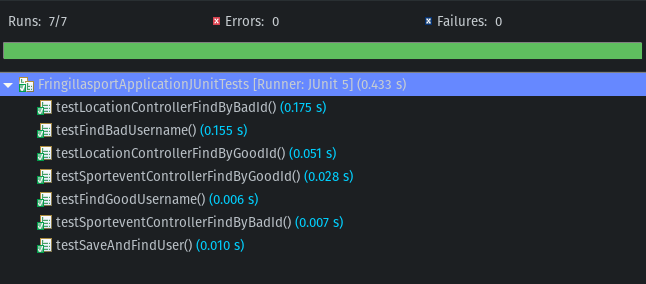
\includegraphics[width=1\linewidth]{slike/JUnitTestovi.PNG}
			\centering
			\caption{rezultati JUnit testova}
			\label{fig:promjene}
		\end{figure}			
			
			\subsection{Ispitivanje sustava}
			
			 Proveli smo ispitivanje sustava koristeći radni okvir Selenium\footnote{\url{https://www.seleniumhq.org/}}.U nastavku ispitujemo 4 ispitna slučaja u kojima testiramo redovne slučajeve, rubne uvjete te namjerno korištenje aplikacije na neočekivani način kako bi se vidjelo na koji način sustav reagira.%Ispitni slučaj se treba sastojati od ulaza (npr. korisničko ime i lozinka), očekivanog izlaza ili rezultata, koraka ispitivanja i dobivenog izlaza ili rezultata.\\ 
			 
			 Za ispitivanje koristili smo alat \textbf{Selenium WebDriver} te programski jezik javu.
			 
			 
			 \hfill\break
			 \noindent\textbf{Ispitni slučaj 1: Prijava u sustav}
			 
			 
			 Da bi korisnik koristio našu web aplikaciju mora se prijaviti u sustav sa već postoječim korisničim računom ili treba prvo napraviti registraciju pa zatim prijavu.
			 Slijedeći test testira prijavu na stranicu sa već postojećim korisničkim računom za sportaša. Nakon uspiješne prijave web aplikacija izbacuje iskočnu poruku koja prikazuje tekst "uspiješna prijava". Funkcionalnost je testirana u metodama testLoginGoodCreds() i testLoginBadCreds().
			 
			 
			 \hfill\break
			 \noindent\textbf{Ulaz:}
			 
			 \begin{packed_enum}
			 	
			 	\item Otvaranje početne stranice u web pregledniku
			 	\item Klik na gumb prijava
			 	\item Unos korisničkog imena
			 	\item Unos lozinke
			 	\item Klik na gumb prijava
			 	
			 	
			 	
			 \end{packed_enum}
			 
			 \noindent\textbf{Očekivani rezultat:}
			 
			 \begin{packed_enum}
			 	
			 	\item Otvorila se početna stranica
			 	\item Prikzala se stranica za prijavu
			 	\item Popunilo se polje za korinsičko ime i šifru
			 	\item Prikazuje se skočna poruka za uspješnu prijavu
			 	\item Prikazuje se profil korisnika
			 	
			 	
			 	
			 \end{packed_enum}
			 
			 \noindent\textbf{Rezultat:} Sva očekivanja su zadovoljena. Selenium test je prošao.
			 
			 
			 \begin{lstlisting}[language=Java,caption={testLoginGoodCreds},label=DescriptiveLabel]	
@Test
void testLoginGoodCreds() {

	System.setProperty("webdriver.chrome.driver", 
	"/Users/Luka/Applications/WebDriver/chromedriver");
	WebDriver driver = new ChromeDriver();

	driver.manage().timeouts().implicitlyWait(10, TimeUnit.SECONDS);
	driver.get("http://localhost:3000/prijava");

	WebElement element = driver.findElement(
	By.xpath("//*[@id=\"root\"]/div/div[2]/div[1]/form/div[1]/div[2]/input"));        
	element.sendKeys("athlete");

	element = driver.findElement(By.xpath(
	"//*[@id=\"root\"]/div/div[2]/div[1]/form/div[2]/div[2]/input"));
	element.sendKeys("athlete");

	driver.findElement(By.xpath(
	"//*[@id=\"root\"]/div/div[2]/div[1]/form/button")).click();

	WebDriverWait wait = new WebDriverWait(driver, 5);
	Alert alert = wait.until(ExpectedConditions.alertIsPresent());
	String alertCheck=alert.getText();
	boolean compRes= alertCheck.contains("Uspjesna");

	assertTrue(compRes);
	driver.quit();
}

			 \end{lstlisting}
			 
			 \hfill\break
			 \noindent\textbf{Ispitni slučaj 2: Prijava s krivim podacima}
		
		Analogni test za prijavu napravili smo i krivim korisničkim podatcima. Očekivani rezultat je poruka upozorenja sa tekstom "Pogreška"
		
			\hfill\break
			\noindent\textbf{Ulaz:}
			
			\begin{packed_enum}
				
				\item Otvaranje početne stranice u web pregledniku
			 	\item Klik na gumb prijava
			 	\item Unos nepostojećeg korisničkog imena
			 	\item Unos nepostojeće lozinke
			 	\item Klik na gumb prijava
				
			\end{packed_enum}
			
			\noindent\textbf{Očekivani rezultat:}
			
			\begin{packed_enum}
				
				\item Otvorila se početna stranica
			 	\item Prikzala se stranica za prijavu
			 	\item Popunilo se polje za korinsičko ime i šifru
			 	\item Prikazuje se skočna poruka za grešku prilikom prijave
				
			\end{packed_enum}
			
			\noindent\textbf{Rezultat:} Sva očekivanja su zadovoljena. Selenium test je prošao.
		
		\begin{lstlisting}[language=Java,caption={testLoginBadCreds},label=DescriptiveLabel]
@Test
void testLoginBadCreds() {
	System.setProperty("webdriver.chrome.driver",
 "/Users/Luka/Applications/WebDriver/chromedriver");
	WebDriver driver = new ChromeDriver();

	driver.manage().timeouts().implicitlyWait(10, TimeUnit.SECONDS);
	driver.get("http://localhost:3000/prijava");

	WebElement element = driver.findElement(By.xpath(
	"//*[@id=\"root\"]/div/div[2]/div[1]/form/div[1]/div[2]/input"));        
	element.sendKeys("wrongUsername");

	element = driver.findElement(By.xpath(
	"//*[@id=\"root\"]/div/div[2]/div[1]/form/div[2]/div[2]/input"));
	element.sendKeys("WrongPassword");

	driver.findElement(By.xpath(
	"//*[@id=\"root\"]/div/div[2]/div[1]/form/button")).click();

	WebDriverWait wait = new WebDriverWait(driver, 5);
	Alert alert = wait.until(ExpectedConditions.alertIsPresent());
	String alertCheck=alert.getText();
	boolean compRes= alertCheck.contains("Pogreska");

	assertTrue(compRes);
	driver.quit();
}

		\end{lstlisting}
		
		\hfill\break
		\noindent\textbf{Ispitni slučaj 3: Prijava na sportsko događanje}
		
		Aplikacija prijavljenim korisnicima nudi mogućnost da se se prijave na neko od nadolazećih sportskih događanja nakon čega sustav prikazje poruku "Uspješno".
		Tu funkcionalnost provjerili smo u klasi SeleniumApplyForEventTest metodom testApplyForEvent.
		
		\hfill\break
		\noindent\textbf{Ulaz:}
		
		\begin{packed_enum}
			
				\item Otvaranje početne stranice u web pregledniku
			 	\item Klik na gumb prijava
			 	\item Unos korisničkog imena
			 	\item Unos lozinke
			 	\item Klik na gumb prijava
			 	\item Klik na gumb karta sportskih okupljanja
			 	\item Klik na prvi event u prikazanoj listi sportskih okupljanja
			 	\item Klik na gumb prijava
			 	\item Klik na gumb za potvrdu prijave
			
		\end{packed_enum}
		
		\noindent\textbf{Očekivani rezultat:}
		
		\begin{packed_enum}
			
				\item Otvorila se početna stranica
			 	\item Prikzala se stranica za prijavu
			 	\item Popunilo se polje za korinsičko ime i šifru
			 	\item Prikazuje se skočna poruka za uspješnu prijavu
			 	\item Prikazuje se stranica s korisnikovim podacima
			 	\item Prikazuje se stranica s kartom i popisom sportskih ikupljanja
			 	\item Prikazuju se detalji o prvom sportskom eventu
			 	\item Prikazuje se skočna poruka za potvrdu prijave
			 	\item Pored sportskog događaja korisniku piše da je prijavljen na njega
			 	
				
				
		\end{packed_enum}
		
		\noindent\textbf{Rezultat:} Sva očekivanja su zadovoljena. Selenium test je prošao.
		
		\begin{lstlisting}[language=Java,caption={testApplyForEvent},label=DescriptiveLabel]
@Test
void testApplyForEvent() {

	System.setProperty("webdriver.chrome.driver",
 "/Users/Luka/Applications/WebDriver/chromedriver");
	WebDriver driver = new ChromeDriver();

	driver.manage().timeouts().implicitlyWait(10, TimeUnit.SECONDS);
	driver.get("http://localhost:3000/prijava");

	WebElement element = driver.findElement(By.xpath(
	"//*[@id=\"root\"]/div/div[2]/div[1]/form/div[1]/div[2]/input"));        
	element.sendKeys("athlete");

	element = driver.findElement(By.xpath(
	"//*[@id=\"root\"]/div/div[2]/div[1]/form/div[2]/div[2]/input"));
	element.sendKeys("athlete");

	driver.findElement(By.xpath(
	"//*[@id=\"root\"]/div/div[2]/div[1]/form/button")).click();

	WebDriverWait wait = new WebDriverWait(driver, 5);
	Alert alert = wait.until(ExpectedConditions.alertIsPresent());
	alert.accept();

	driver.findElement(By.xpath(
	"//*[@id=\"root\"]/div/div[1]/nav/ul/li[2]/a")).click();
	
	driver.findElement(By.xpath(
	"//*[@id=\"root\"]/div/div[2]/div[2]/div[1]/div/h3")).click();
	
	driver.findElement(By.xpath(
	"//*[@id=\"root\"]/div/div[2]/div[2]/div[3]/p")).click();

	Alert alert2 = wait.until(ExpectedConditions.alertIsPresent());
	alert2.accept();
	Alert alert3 = wait.until(ExpectedConditions.alertIsPresent());
	boolean checker = alert3.getText().contains("Uspjesno");

	assertTrue(checker);
	driver.quit();
}

		\end{lstlisting}
		
		\hfill\break
		\noindent\textbf{Ispitni slučaj 4: Stvaranje sportske lokacije}
		
		Osim prijave na već postojeća sportska događanja, korisnik može u sustav i dodati novu lokaciju na kojoj će se održavati sportska okupljanja.
		Tu funkcionalnost isprobali smo u klasi SeleniumCreateLocationTest u metodi testCreateLocation().
		Stvorena je lokacija pod nazivom "TestnaLokacija".
		Da bi dodali tu lokaciju simulirali smo klikove na karti kojima bi označili poligon, odnosno površinu koju ta lokacija zauzima na karti.
		
		
		\hfill\break
		\noindent\textbf{Ulaz:}
		
		\begin{packed_enum}
			
				\item Otvaranje početne stranice u web pregledniku
			 	\item Klik na gumb prijava
			 	\item Unos korisničkog imena
			 	\item Unos lozinke
			 	\item Klik na gumb prijava
			 	\item Klik na gumb stvori sportsku lokaciju
			 	\item Klik na gumb za približavanje karte
			 	\item Klik na gumb za početak ucrtavanja lokacije
			 	\item Odabir 4 točke na mapi
			 	\item Klik na gumb za završetak ucrtavanja lokacije
			 	\item Upis imena lokacije
			 	\item Klik na gumb stvori novu lokaciju
			
		\end{packed_enum}
		
		\noindent\textbf{Očekivani rezultat:}
		
		\begin{packed_enum}
			
				\item Otvorila se početna stranica
			 	\item Prikzala se stranica za prijavu
			 	\item Popunilo se polje za korinsičko ime i šifru
			 	\item Prikazuje se skočna poruka za uspješnu prijavu
			 	\item Prikazuje se stranica s korisnikovim podacima
			 	\item Prikazuje se stranica za kreiranje nove sportske lokacije
			 	\item Karta se približi
			 	\item Odaberu se 4 točke na karti
			 	\item Unosi se ime lokacije
			 	\item Prikazuje se skočna poruka o uspješnom kreiranju sportske lokacije
			
		\end{packed_enum}
		
		\noindent\textbf{Rezultat:} Sva očekivanja su zadovoljena. Selenium test je prošao.
		
		\begin{lstlisting}[language=Java,caption={testCreateLocation},label=DescriptiveLabel]
@Test
void testCreateLocation() {
		
	System.setProperty("webdriver.chrome.driver",
 "/Users/Luka/Applications/WebDriver/chromedriver");
	WebDriver driver = new ChromeDriver();

	driver.manage().timeouts().implicitlyWait(10, TimeUnit.SECONDS);
	driver.get("http://localhost:3000/prijava");
	
	WebElement element = driver.findElement(By.xpath(
	"//*[@id=\"root\"]/div/div[2]/div[1]/form/div[1]/div[2]/input"));  
    
	element.sendKeys("athlete");
	element = driver.findElement(By.xpath("
	//*[@id=\"root\"]/div/div[2]/div[1]/form/div[2]/div[2]/input"));
	
	element.sendKeys("athlete");
	driver.findElement(By.xpath("
	//*[@id=\"root\"]/div/div[2]/div[1]/form/button")).click();

	WebDriverWait wait = new WebDriverWait(driver, 5);
	Alert alert = wait.until(ExpectedConditions.alertIsPresent());
	alert.accept();
	
	//Stvori lokaciju
	driver.findElement(By.xpath("
	//*[@id=\"root\"]/div/div[1]/nav/ul/li[3]/a")).click();
	
	//zoom x2
	driver.findElement(By.xpath("
	//*[@id=\"root\"]/div/div[2]/div/div[2]/div[1]/div/a[1]")).click();
	
	driver.findElement(By.xpath("
	//*[@id=\"root\"]/div/div[2]/div/div[2]/div[1]/div/a[1]")).click();
	
	//polygon button
	driver.findElement(By.xpath("
	//*[@id=\"root\"]/div/div[2]/div/div[2]/div[2]/div/div[1]/div/a")).click();

	Actions actions = new Actions(driver);
	actions.moveToElement(driver.findElement(By.xpath("
	//*[@id=\"root\"]/div/div[2]/div")), 0, 0);
	
	actions.moveByOffset(150, 75).click().build().perform();
	actions.moveByOffset(0, 30).click().build().perform();
	actions.moveByOffset(30, 0).click().build().perform();
	actions.moveByOffset(0, -30).click().build().perform();
	
	//finish
	driver.findElement(By.xpath("
	//*[@id=\"root\"]/div/div[2]/div/div[2]/div[2]/div/div[1]/ul/li[1]/a")).click();
	
	//ime lokacije
	driver.findElement(By.xpath("
	//*[@id=\"root\"]/div/div[2]/form/input")).sendKeys("TestnaLokacija");
	
	//Zavrsi
	driver.findElement(By.xpath("//*[@id=\"root\"]/div/div[2]/form/h3")).click();
	
	Alert alert3 = wait.until(ExpectedConditions.alertIsPresent());
	boolean checker = alert3.getText().contains("uspjesno");


	assertTrue(checker);
	driver.quit();
}

		\end{lstlisting}
		
		\hfill\break
		\noindent\textbf{Ispitni slučaj 5: Pogrešno stvaranje nove lokacije}
		
		Proveli smo  još jedan test sa dodavanjem lokacije, ali bez da smo "kliknuli" odnosno specificirali gde na karti se ta lokacija nalazi pa zbog toga naravno očekujemo grešku.
		
		\hfill\break
		\noindent\textbf{Ulaz:}
		
		\begin{packed_enum}
			
				\item Otvaranje početne stranice u web pregledniku
			 	\item Klik na gumb prijava
			 	\item Unos korisničkog imena
			 	\item Unos lozinke
			 	\item Klik na gumb prijava
			 	\item Klik na gumb stvori sportsku lokaciju
			 	\item Upis imena lokacije
			 	\item Klik na gumb stvori novu lokaciju
			
		\end{packed_enum}
		
		\noindent\textbf{Očekivani rezultat:}
		
		\begin{packed_enum}
			
				\item Otvorila se početna stranica
			 	\item Prikzala se stranica za prijavu
			 	\item Popunilo se polje za korinsičko ime i šifru
			 	\item Prikazuje se skočna poruka za uspješnu prijavu
			 	\item Prikazuje se stranica s korisnikovim podacima
			 	\item Prikazuje se stranica za kreiranje nove sportske lokacije
			 	\item Unosi se ime lokacije
			 	\item Prikazuje se skočna poruka o neuspješnom kreiranju sportske lokacije
			
		\end{packed_enum}
		
		\noindent\textbf{Rezultat:} Sva očekivanja su zadovoljena. Selenium test je prošao.
		
		\begin{lstlisting}[language=Java,caption={testCreateLocation},label=DescriptiveLabel]
		
@Test
void testCreateLocation() {
		
	System.setProperty("webdriver.chrome.driver",
 "/Users/Luka/Applications/WebDriver/chromedriver");
	WebDriver driver = new ChromeDriver();

	driver.manage().timeouts().implicitlyWait(10, TimeUnit.SECONDS);
	driver.get("http://localhost:3000/prijava");
	
	WebElement element = driver.findElement(By.xpath(
	"//*[@id=\"root\"]/div/div[2]/div[1]/form/div[1]/div[2]/input")); 
     
	element.sendKeys("athlete");
	element = driver.findElement(By.xpath(
	"//*[@id=\"root\"]/div/div[2]/div[1]/form/div[2]/div[2]/input"));
	
	element.sendKeys("athlete");
	driver.findElement(By.xpath(
	"//*[@id=\"root\"]/div/div[2]/div[1]/form/button")).click();

	WebDriverWait wait = new WebDriverWait(driver, 5);
	Alert alert = wait.until(ExpectedConditions.alertIsPresent());
	alert.accept();
	
	//Stvori lokaciju
	driver.findElement(By.xpath(
	"//*[@id=\"root\"]/div/div[1]/nav/ul/li[3]/a")).click();
	
	
	//ime lokacije
	driver.findElement(By.xpath(
	"//*[@id=\"root\"]/div/div[2]/form/input")).sendKeys("TestnaLokacija");
	
	//Zavrsi
	driver.findElement(By.xpath(
	"//*[@id=\"root\"]/div/div[2]/form/h3")).click();
	
	Alert alert3 = wait.until(ExpectedConditions.alertIsPresent());
	boolean checker = alert3.getText().contains("pogreske");

	assertTrue(checker);
	driver.quit();
}

		
		\end{lstlisting}
		
		\eject
		
		
		\section{Dijagram razmještaja}
			Dijagram razmještaja na slici prikazuje odnos sklopovlja i programske potpore na njemu. Na korisničkom računalu web preglednik HTTP protokolom pristupa web aplikaciji na poslužiteljskom računalu. Na poslužiteljskom računalu nalaze se Web poslužitelj na kojem je pokrenuta web aplikacija te poslužitelj baze podataka na kojem se nalazi baza podataka. Također nalazi se i poslučitelj strojnog učenja na kojemu se nalazi predikcija sporta strojnim učenjem. Korisniku potrebne podatke dostavlja web aplikacija koja ih dobiva komunikacijom s bazom podataka i s predikcijom strojnog učenja.
			
			\begin{figure}[H]
				 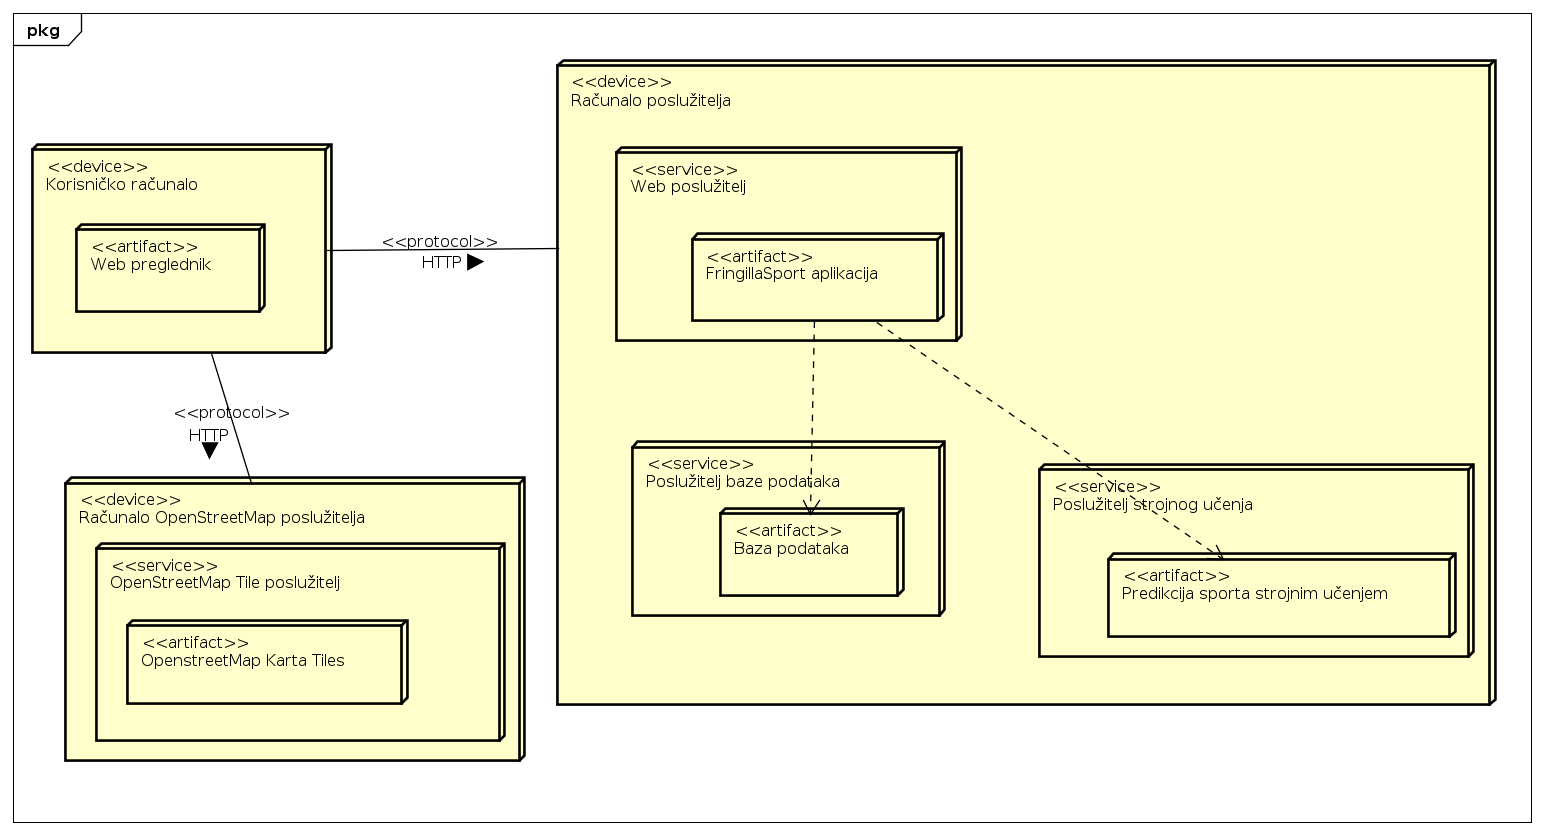
\includegraphics[width=\textwidth]{dijagrami/DeploymentDiagram0.png}
				 \caption{Dijagram razmještaja}
			\end{figure}
			
			\eject 
		
		\section{Upute za puštanje u pogon}
		
			Aplikacija je puštena u pogon na ubuntu 18.04 serveru. Te je na serveru potrebno imati instaliranu Javu 11.0, Node.js i Python 3.0.
			
			\subsection{Instalacija postgresql baze podataka}
			Potrebno je instalirati postgresql bazu podataka s naredbom:
			\begin{verbatim}
				$ sudo apt install postgresql postgresql-contrib
			\end{verbatim}
			Potom kreiramo bazu podataka za aplikaciju:
			\begin{verbatim}
				$ createdb-h localhost -p 5432 -U postgres fringilladb password pass
			\end{verbatim}
			Navedene podatke potrebno je unjesti u datoteku backenda na lokaciji backend/src/main/resources/application.properties:
			
			\begin{verbatim}
			spring.datasource.url=jdbc:postgresql://localhost:5432/fringilladb
			spring.datasource.username=postgres
			spring.datasource.password=pass
			spring.jpa.hibernate.dll-auto=create
			\end{verbatim}
			
			\subsection{Instalacija drugih potrebnih paketa}
			
			Za ostale komponente aplikacije potrebno je instalirati programe navedenim naredbama.
			
			\begin{verbatim}
				$ sudo apt install software-properties-common
				$ sudo apt install nodejs python3 python3-pip default-jre
			\end{verbatim}
		
			\subsection{Pokretanje backenda}
			Potrebno se je pozicionirati u direktorij izvorniKod/backend te pokrenuti naredbu:
			\begin{verbatim}
				$ ./mvn spring-boot:run
			\end{verbatim}
			
			\subsection{Pokretanje frontenda}
			Frontend aplikacije pokrece se pozicioniranjem u direktorij izvorniKod/frontend te izvršavanjem naredbi:
			
			\begin{verbatim}
				$ npm install
				$ npm start
			\end{verbatim}
			Prva naredba instalira potrebne pakete, dok druga pokreće frontend. 
			
			\subsection{Pokretanje servera za predlaganje sporta}

			Za pokretanje python servera potrebno se je pozicionirati u direktorij izvorniKod/mlSportPredict te pokrenuti naredbu:
			
			\begin{verbatim}
				$ python server.py
			\end{verbatim}
			
			
			Napomena zbog trenutne konfiguracije potrebno je stvoriti link između direktorija izvorniKod/backend/uploads i izvorniKod/frontend/public/documentation.
			
			\eject 

	\chapter{Zaključak i budući rad}
		
		Naša grupa imala je zadatak izraditi aplikaciju koja omogućuje jednostavnije povezivanje sportaša, trenera i iznajmljivača sportskih prostora te taj proces pojednostavljuje i ubrzava. Ideja aplikacije je proizašla od članova naše grupe, zbog toga su svi članovi bili dodatno motivirani da uspješno i kvalitetno izradimo aplikaciju te uz nju napišemo kvalitetnu dokumentaciju. 
		
		Za izradu ove aplikacije odlučili smo se koristiti tehnologije Spring Boot za backend, te React za frontend. Najveći izazov je bio naučiti koristiti navedene tehnologije te povezati frontend i backend. Da bismo lakše prevladali ovaj izazov podijelili smo grupu u 2 manja tima, jedan za frontend te jedan za backend, svaki tim je sadržavao po 3 člana naše grupe. Voditelj naše grupe je vodio oba tima, zbog toga su timovi tijekom cijelog projekta bili cijelo vrijeme na istoj razini te ni jedan tim nije zaostajao za drugim. Ovakav raspored te dobra atmosfera i komunikacija među članovima učinila je rad cijele grupe produktivnijim te s time i olakšala prevladavanje svih izazova i prepreka.
		
		Projekt je bio podijeljen u dvije faze kroz 15 tjedana. Prva faza je uključivala okupljanje tima, smišljanja ideje za aplikaciju, podjelu u timove, dodjelu projektnog zadatka, rad na dokumentaciji i implementaciju osnovnih funkcionalnosti aplikacije. Druga faza je uključivala završetak svih funkcionalnosti backenda i frontenda, testiranje aplikacije te dovršetak dokumentacije i cijelog projekta.
		
		Prilikom izrade ovog projekta naučili smo uz dosada navede tehnologije koristiti sustav za upravljanje izvornim kodom Git te alate TEXstudio i Astah koji služe za pisanje dokumentacije i crtanje dijagrama. Osim navedenih tehnologija naučili smo pisati kvalitetnu dokumentaciju te kvalitno oblikovati kod koji je iznimno važan za daljnu nadogradnju projekta, testiranje i tražanje grešaka u kodu. Možda i najvažnija lekcija naučena prilikom izrade ovog projekta je važnost grupnog rada, ispunjavanje svojih obaveza na vrijeme te suradnja i komunikacijama s kolegama. Sve navedene naučene lekcije su od iznimne važnosti za naš daljni razvoj i uspješnost u struci.
		
		
		Za brže i kvalitetnije ostvaranje projekta potrebno je imati već određeno iskustvo u korištenim tehnologijama te iskustvo u sličnim projektima. Osim toga, jako je važno raditi na što manje projekata paralelno, na taj način imali bi više vremena i veći fokus za naš.
		
		Naša aplikacija "FringillaSport" mogla bi se nadograditi na brojne načine. Jedna od ideja za dodatne funkcionalnosti je ocjenjivanje sportaša, trenera te prostora za sport, sportaši bi nakon sudjelovanja na nekom događaju mogli ocijeniti ostale sportaše, trenera te prostor za sport s ciljem kvalitetnije usluge aplikacije i informacijama o kvaliteti sportskih događaja.
		
		
		
%	\chapter*{Popis literature}
		\addcontentsline{toc}{chapter}{Popis literature}
	 	
 		\textbf{\textit{Kontinuirano osvježavanje}}
	
		\textit{Popisati sve reference i literaturu koja je pomogla pri ostvarivanju projekta.}
		
		
		\begin{enumerate}
			
			
			\item  Programsko inženjerstvo, FER ZEMRIS, \url{http://www.fer.hr/predmet/proinz}
			
			\item  I. Sommerville, "Software engineering", 8th ed, Addison Wesley, 2007.
			
			\item  T.C.Lethbridge, R.Langaniere, "Object-Oriented Software Engineering", 2nd ed. McGraw-Hill, 2005.
			
			\item  I. Marsic, Software engineering book``, Department of Electrical and Computer Engineering, Rutgers University, \url{http://www.ece.rutgers.edu/~marsic/books/SE}
			
			\item  The Unified Modeling Language, \url{https://www.uml-diagrams.org/}
			
			\item  Astah Community, \url{http://astah.net/editions/uml-new}
		\end{enumerate}
		
		 
	
	
%	\begingroup
%	\renewcommand*\listfigurename{Indeks slika i dijagrama}
%	%\renewcommand*\listtablename{Indeks tablica}
%	%\let\clearpage\relax
%	\listoffigures
%	%\vspace{10mm}
%	%\listoftables
%	\endgroup
%	\addcontentsline{toc}{chapter}{Indeks slika i dijagrama}


	
%	\eject 
		
	\chapter*{Dodatak: Prikaz aktivnosti grupe}
		\addcontentsline{toc}{chapter}{Dodatak: Prikaz aktivnosti grupe}
		
		\section*{Dnevnik sastajanja}
		
		\textbf{\textit{Kontinuirano osvježavanje}}\\
		
		 \textit{U ovom dijelu potrebno je redovito osvježavati dnevnik sastajanja prema predlošku.}
		
		\begin{packed_enum}
			\item  sastanak
			\item[] \begin{packed_item}
				\item Datum: 5. listopada 2020.
				\item Prisustvovali: G.Crnogorac, L.Ilić, M.Marfat, L.Nuić, B.Paradžik, M.Rašić, L.Srdarev
				\item Teme sastanka:
				\begin{packed_item}
					\item  sastanak a asistentom
					\item  objašnjenje zadatka
					\item  rasprava o predloženom zadatku
				\end{packed_item}
			\end{packed_item}
			
			\item  sastanak
			\item[] \begin{packed_item}
				\item Datum: 17. listopada 2020.
				\item Prisustvovali: G.Crnogorac, L.Ilić, M.Marfat, L.Nuić, B.Paradžik, M.Rašić, L.Srdarev
				\item Teme sastanka:
				\begin{packed_item}
					\item  rasprava o funkcionalnim zahtjevima i obrascima uporabe
					\item  razgovor o iskustvima pojedinih članova u različitim tehnologijama
				\end{packed_item}
			\end{packed_item}
			
			\item  sastanak
			\item[] \begin{packed_item}
				\item Datum: 19. listopada 2020.
				\item Prisustvovali: G.Crnogorac, L.Ilić, M.Marfat, L.Nuić, B.Paradžik, M.Rašić, L.Srdarev
				\item Teme sastanka:
				\begin{packed_item}
					\item  sastanak s asistentom 
					\item  dogovor o tehnologijama koje će se koristiti u projektu
				\end{packed_item}
			\end{packed_item}
			
			\item  sastanak
			\item[] \begin{packed_item}
				\item Datum: 28. listopada 2020.
				\item Prisustvovali: G.Crnogorac, L.Ilić, M.Marfat, L.Nuić, B.Paradžik, M.Rašić, L.Srdarev
				\item Teme sastanka:
				\begin{packed_item}
					\item  dogovor o daljnoj podjeli zadataka
					\item  rasprava o bazi podataka
				\end{packed_item}
			\end{packed_item}
			
			\item  sastanak
			\item[] \begin{packed_item}
				\item Datum: 5. studenoga 2020.
				\item Prisustvovali: G.Crnogorac, L.Ilić, M.Marfat, L.Nuić, B.Paradžik, M.Rašić, L.Srdarev
				\item Teme sastanka:
				\begin{packed_item}
					\item  povezivanje frontenda i backenda
					\item  detaljnija rasprava o bazi podataka
				\end{packed_item}
			\end{packed_item}	
			
			\item  sastanak
			\item[] \begin{packed_item}
				\item Datum: 9. studenoga 2020.
				\item Prisustvovali: M.Marfat, L.Nuić, M.Rašić, L.Srdarev
				\item Teme sastanka:
				\begin{packed_item}
					\item  sastanak s asistentom
					\item  pregled dosadašnjeg rada
				\end{packed_item}
			\end{packed_item}
		
			\item  sastanak
			\item[] \begin{packed_item}
				\item Datum: 2. prosinca 2020.
				\item Prisustvovali:  G.Crnogorac, L.Ilić, M.Marfat, L.Nuić, B.Paradžik, M.Rašić, L.Srdarev 
				\item Teme sastanka:
				\begin{packed_item}
					\item  sastanak s asistenticom - evaluacija dosadašnjeg rada
				\end{packed_item}
			\end{packed_item}
		
			\item  sastanak
			\item[] \begin{packed_item}
				\item Datum: 23. prosinca 2020.
				\item Prisustvovali:  G.Crnogorac, L.Ilić, M.Marfat, L.Nuić, B.Paradžik, M.Rašić, L.Srdarev 
				\item Teme sastanka:
				\begin{packed_item}
					\item  pregled napravljenog dijela projekta
					\item  plan nastavka projekta
					\item  podjela zadataka  
				\end{packed_item}
			\end{packed_item}
		
			\item  sastanak
			\item[] \begin{packed_item}
				\item Datum: 29. prosinca 2020.
				\item Prisustvovali:  G.Crnogorac, L.Ilić, M.Marfat, L.Nuić, M.Rašić, L.Srdarev, B.Paradžik
				\item Teme sastanka:
				\begin{packed_item}
					\item  pregled napravljenog od zadnjeg sastanka 
					\item  podjela novih zadataka za backend i frontend 
				\end{packed_item}
			\end{packed_item}
		
			\item  sastanak
			\item[] \begin{packed_item}
				\item Datum: 2. siječnja 2021.
				\item Prisustvovali:  G.Crnogorac, L.Ilić, M.Marfat, L.Nuić, M.Rašić, L.Srdarev 
				\item Teme sastanka:
				\begin{packed_item}
					\item  pregled napravljenog od zadnjeg sastanka 
					\item  podjela novih zadataka za backend i frontend
				\end{packed_item}
			\end{packed_item}
		
			\item  sastanak
			\item[] \begin{packed_item}
				\item Datum: 4. siječnja 2021.
				\item Prisustvovali: L.Ilić, L.Nuić, B.Paradžik, L.Srdarev
				\item Teme sastanka:
				\begin{packed_item}
					\item  pregled napravljenih funkcionalnosti backenda 
					\item  rješavanje dosadašnjih problema u implementaciji backenda
				\end{packed_item}
			\end{packed_item}
		
			\item  sastanak
			\item[] \begin{packed_item}
				\item Datum: 4. siječnja 2021.
				\item Prisustvovali: G.Crnogorac,  M.Marfat, L.Nuić, M.Rašić
				\item Teme sastanka:
				\begin{packed_item}
					\item  pregled napravljenih funkcionalnosti frontenda 
					\item  podjela novih zadataka za frontend
				\end{packed_item}
			\end{packed_item}
		
			\item  sastanak
			\item[] \begin{packed_item}
				\item Datum: 6. siječnja 2021.
				\item Prisustvovali: G.Crnogorac, L.Ilić, M.Marfat, L.Nuić, M.Rašić, L.Srdarev, B.Paradžik
				\item Teme sastanka:
				\begin{packed_item}
					\item  pregled napravljenih funkcionalnosti backenda 
					\item  pregled rada aplikacije
					\item  utvrđvanje i rješavanje
					 grešaka aplikacije
					\item  aktualizacija dokumentacije
				\end{packed_item}
			\end{packed_item}
		
			\item  sastanak
			\item[] \begin{packed_item}
				\item Datum: 7. siječnja 2021.
				\item Prisustvovali: G.Crnogorac, L.Ilić, M.Marfat, L.Nuić, M.Rašić, L.Srdarev, B.Paradžik
				\item Teme sastanka:
				\begin{packed_item}
					\item  sastanak s asistentom - demonstracija alfa inacice
				\end{packed_item}
			\end{packed_item}
		
			
			
			
			
			%
			
		\end{packed_enum}
		
		\eject
		\section*{Tablica aktivnosti}
		
			\textbf{\textit{Kontinuirano osvježavanje}}\\
			
			 \textit{Napomena: Doprinose u aktivnostima treba navesti u satima po članovima grupe po aktivnosti.}
					
						
			
			\begin{longtabu} to \textwidth {|X[7, l]|X[1, c]|X[1, c]|X[1, c]|X[1, c]|X[1, c]|X[1, c]|X[1, c]|}
								
				\cline{2-8} \multicolumn{1}{c|}{\textbf{}} &     \multicolumn{1}{c|}{\rotatebox{90}{\textbf{Lovro Nuić }}} & \multicolumn{1}{c|}{\rotatebox{90}{\textbf{Grgur Crnogorac }}} &	\multicolumn{1}{c|}{\rotatebox{90}{\textbf{Luka Ilić }}} &	\multicolumn{1}{c|}{\rotatebox{90}{\textbf{Marko Marfat }}} &
				\multicolumn{1}{c|}{\rotatebox{90}{\textbf{Berislav Paradžik }}} &
				\multicolumn{1}{c|}{\rotatebox{90}{\textbf{Marin Rašić }}} &	\multicolumn{1}{c|}{\rotatebox{90}{\textbf{Luka Srdarev }}} \\ \hline 
				\endfirsthead
				
			
				\cline{2-8} \multicolumn{1}{c|}{\textbf{}} &     \multicolumn{1}{c|}{\rotatebox{90}{\textbf{Lovro Nuić }}} & \multicolumn{1}{c|}{\rotatebox{90}{\textbf{Grgur Crnogorac }}} &	\multicolumn{1}{c|}{\rotatebox{90}{\textbf{Luka Ilić }}} &
				\multicolumn{1}{c|}{\rotatebox{90}{\textbf{Marko Marfat }}} &	\multicolumn{1}{c|}{\rotatebox{90}{\textbf{Berislav Paradžik }}} &
				\multicolumn{1}{c|}{\rotatebox{90}{\textbf{Marin Rašić }}} &	\multicolumn{1}{c|}{\rotatebox{90}{\textbf{Luka Srdarev }}} \\ \hline 
				\endhead
				
				
				\endfoot
							
				 
				\endlastfoot
				
				Upravljanje projektom 		& 10 &  &  &  &  &  & \\ \hline
				Opis projektnog zadatka 	&  &  &  &  & 2 & 3 & \\ \hline
				
				Funkcionalni zahtjevi       &  &  & 1 & 1 &  & 1 &  \\ \hline
				Opis pojedinih obrazaca 	&  &  & 1 & 1 &  & 1 &  \\ \hline
				Dijagram obrazaca 			&  & 4 &  &  &  &  &  \\ \hline
				Sekvencijski dijagrami 		&  &  &  & 3 &  &  &  \\ \hline
				Opis ostalih zahtjeva 		&  &  &  & 1 &  &  &  \\ \hline

				Arhitektura i dizajn sustava	 &  &  & 3 &  &  &  & 8 \\ \hline
				Baza podataka				&  &  & 4 &  &  &  & 10  \\ \hline
				Dijagram razreda 			& 10 &  &  &  &  &  &   \\ \hline
				Dijagram stanja				&  &  &  &  &  &  &  \\ \hline
				Dijagram aktivnosti 		&  &  &  &  &  &  &  \\ \hline
				Dijagram komponenti			&  & 1.5 &  &  &  &  &  \\ \hline
				Korištene tehnologije i alati 		&  &  &  &  &  &  &  \\ \hline
				Ispitivanje programskog rješenja 	&  &  & 12 &  &  &  & 12 \\ \hline
				Dijagram razmještaja			&  & 1.5 &  &  &  &  &  \\ \hline
				Upute za puštanje u pogon 		& 1 &  &  &  &  &  &  \\ \hline 
				Dnevnik sastajanja 			& 1 &  &  &  &  & 0.5  &  \\ \hline
				Zaključak i budući rad 		&  &  &  &  &  &  &  \\  \hline
				Popis literature 			&  &  &  &  &  &  &  \\  \hline
				&  &  &  &  &  &  &  \\  \hline
				&  &  &  &  &  &  &  \\ \hline \hline
				\textit{Backend} 	& 80 &  & 25 &  & 4 &  & 25 \\  \hline
				\textit{Frontend} 	&  & 45 &  & 35 &  & 40 &  \\  \hline
				 							&  &  &  &  &  &  &\\  \hline
				
				
			\end{longtabu}
					
					
		\eject
		\section*{Dijagrami pregleda promjena}

		\begin{figure}[H]
			\centering
			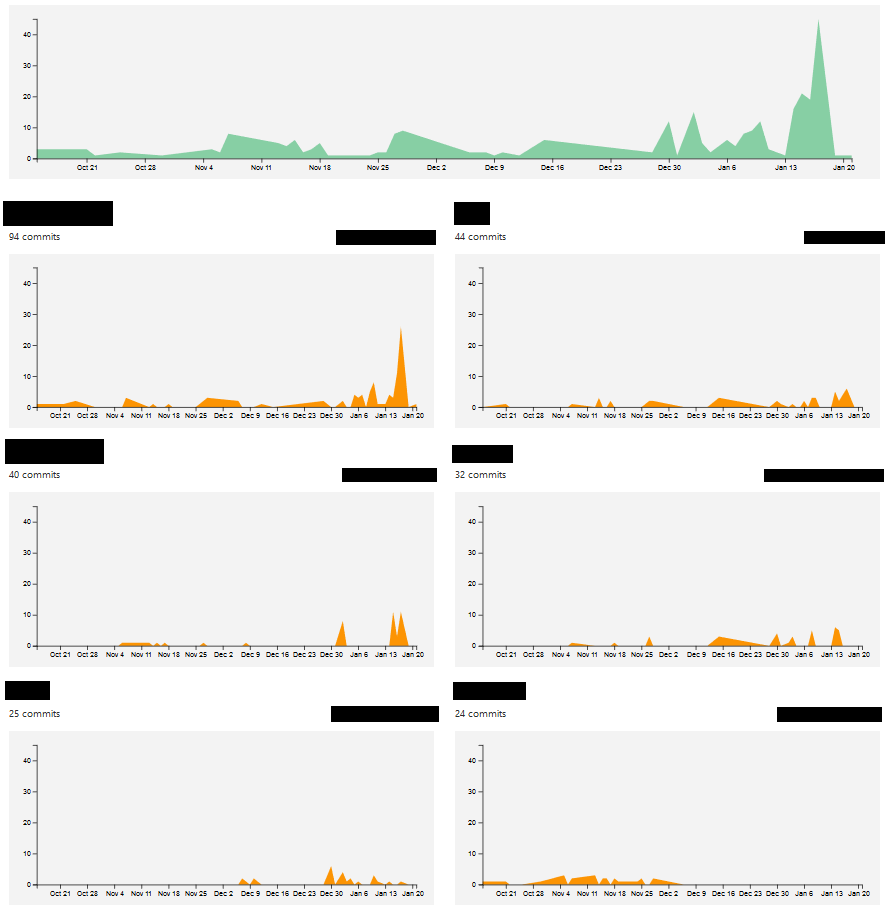
\includegraphics[scale=0.6]{slike/aktivnost.png}
			\caption{Dijagram pregleda promjena}
		\end{figure}
		
%		\textbf{\textit{dio 2. revizije}}\\
		
%		\textit{Prenijeti dijagram pregleda promjena nad datotekama projekta. Potrebno je na kraju projekta generirane grafove s gitlaba prenijeti u ovo poglavlje dokumentacije. Dijagrami za vlastiti projekt se mogu preuzeti s gitlab.com stranice, u izborniku Repository, pritiskom na stavku Contributors.}
		
	


\end{document} %naredbe i tekst nakon ove naredbe ne ulaze u izgrađen dokument 


